\documentclass[a4paper,12pt,twoside,openright]{book}
\usepackage{preamble}
\usepackage{pgf}


\author{Yohann Faure}
\title{\centering
	\textbf{
		\LARGE 
			\textcolor{BrickRed}{Dynamique d'une faille en laboratoire}\\
		\vspace{.3cm}
		\Large
			\textcolor{black}{~~Étude de l'influence d'un milieu granulaire}
	}
}



\begin{document}


%\include{PDG.tex}
%\thispagestyle{empty}

\include{PDG.tex}
%\newgeometry{
	textheight = 265 mm,
	left = 25 mm,
	right = 25 mm,
	heightrounded,
}

\begin{titlepage}

\includegraphics[height=0.2\textwidth]{../logos/logocnrs.pdf}\hfill
\includegraphics[height=0.2\textwidth]{../logos/logolabo.pdf}

 
	\begin{center}
		
		\vspace{10pt}
		
		{\LARGE\textbf{TH\`ESE DE DOCTORAT} \\
		\vspace{1pt}
		\Large\textbf{de l'\textsc{Université de Lyon}} \\
		\vspace{.08cm}
		\large{opérée par}\\
		\vspace{.1cm}
		\Large\textbf{l'\textsc{\'Ecole Normale Supérieure de Lyon}}
		}
		
		
		\vspace{35pt}
		
		{\large \textbf{\'Ecole Doctorale \textsc{n}\textsuperscript{o}\,52}\\
		{\large{Physique et Astrophysique}}}
		
		\vspace{20pt}
		
		{\large Discipline : \textbf{Physique}}
		
		\vspace{30pt}
		
		Soutenue publiquement le mercredi 17 juillet 2024, par\\
		
		\vspace{15pt}
		
		{\LARGE\textbf{Yohann \textsc{Faure}}}\\
	\end{center}
	
	\vspace{10pt}
	
	\begin{center}
		\noindent\rule{16cm}{0.25pt}\\
		\vspace{10pt}
		{\THETITLE } \\
		%\vspace{20pt}
		\noindent\rule{16cm}{0.25pt}\\
	\end{center}
	\vfill 
	
	%%%%%%%%%%%%%%%%% Avec affiliations %%%%%%%%%%%%%%%%%%%%%%%%%%%% 
	
	\noindent { Devant le jury compos\'e de :} \\
	
	\noindent \begin{tabular}{p{0.3\textwidth}p{0.4\textwidth}p{0.3\textwidth}}
		Jérôme \textsc {Crassous} & 
			Professeur des Universités & 
			Rapporteur
		\\
			&
			IPR (Rennes)  & \\
		Julien \textsc {Scheibert} & Directeur de Recherche CNRS & Rapporteur\\
		& LTDS (Lyon) & \\
		Marianne \textsc {Métois} &  Maîtresse de Conférences & Examinatrice \\
		& LGLTPE (Lyon)& \\
		François \textsc {Passelègue} & Chargé de Recherche CNRS & Examinateur\\
		& Géoazur (Nice) & \\
		Elsa \textsc {Bayart} & Chargée de Recherche CNRS & Co-directrice de thèse\\
		& LPENSL (Lyon) &\\
		Mokhtar \textsc {Adda-Bedia} & Directeur de Recherche CNRS & Co-directeur de thèse\\
		& LPENSL (Lyon) &
	\end{tabular}
	
\end{titlepage}

\restoregeometry 


%\newpage
%~~
%\newpage
%~~
%\newpage
\newpage



\newgeometry{twoside,inner=2.5cm,outer=1.5cm,top=2cm, bottom=1.5cm, headsep=0.5cm}
\pagestyle{fancy}
\setlength{\headheight}{20pt}
\fancyhead[LE,RO]{\thepage}
\fancyhead[LO]{\rightmark}
\fancyhead[RE]{\leftmark}
\fancyfoot{}


%\cleardoublepage

\fancypagestyle{plain}{% first page of chapters
    \fancyhf{}
    \fancyhead[LE,RO]{}
    \renewcommand{\headrulewidth}{0pt}
}
\include{chap_resume.tex}

\newpage

{ \let\cleardoublepage\relax
\chapter*{Abstract}}
\thispagestyle{empty}

When two tectonic plates in contact move relative to each other, an increasing shear force is applied to their interface, the seismic fault, which eventually starts slipping, giving rise to an earthquake that releases the stored elastic energy. The study of these movements on a global scale is carried out in situ using seismic or geodetic measurements, but as well as being highly heterogeneous, the interfaces studied are not directly accessible. Laboratory experiments can be used to study the behaviour of model faults formed by samples of rocks or plastic materials by isolating the parameters that play a role in their dynamics. The aim of our study is to identify the influence of a layer of gouge, a crushed rock present at the interface in powder or grain form, on the behaviour of a seismic fault.


To do this, we developed an experimental device for shearing a frictional interface, enabling us to measure deformations and track particles at high frequency. This allowed us to perform various experiments on two-dimensional frictional interfaces formed by solid blocks of PMMA in the presence of a granular medium trapped at the interface, modelling the gouge. In particular, we studied the interaction mechanisms between a slowly slipping portion of a fault and the surrounding locked regions. Our results show that the slowly slipping portion acts as a precursor to rupture events, destabilising the interface by a mechanism similar to that of a pre-crack in a homogeneous solid. This result and this versatile experimental set-up pave the way for new perspectives in the study of complex frictional interfaces.


\newpage

%{ \let\cleardoublepage\relax

\chapter*{Remerciements} }
\thispagestyle{empty}


Voici venu l'exercice difficile des remerciements. On va pas se mentir, remercier toutes les personnes qui m'ont accompagné, parfois aidé, beaucoup soutenu, et souvent supporté pendant ces dernières années serait long. Si vous n'êtes pas dans la liste, vous pouvez m'envoyer un message pour m'engueuler, on en profitera pour se planifier une sortie en ville !


\vskip 2cm

\subsection*{La Recherche}
Tout d'abord, chers membres du Jury, J.\,Crassous, J.\,Scheibert, M.\,Métois et F.\,Passelègue, je vous remercie d'avoir accepté d'évaluer mon travail. Vous faites partie des rares personnes qui ont lu ce manuscript en entier, et vos remarques ont été précieuses pour sa finalisation. En m'ayant jugé digne du titre de Docteur, vous m'avez offert l'honneur de me considérer comme un collègue, ce qui, au delà des formalités de mise dans ce type d'exercice, me touche sincèrement.

\vskip 1cm

Elsa,
\vskip .5cm

Voilà maintenant trois ans que nous naviguons ensemble. Trois années durant lesquelles tu m'as ouvert la porte du monde de la recherche et m'a guidé dans ses eaux tumultueuses. Tu savais dès le départ que je comptais après ma thèse quitter cet océan pour retourner patauger dans la mer \texttt{tranquille} de l'Éducation Nationale, et pourtant tu as tout fait pour me pousser à donner le meilleur de moi-même, m'encourageant à y rester. Nous avons bien sûr eu nos différents, et avons dû nous ajuster à nos méthodes respectives pour conserver le navire à flôt, mais le mât à tenu bon. Ces trois années passées au large, nous avons été secoués par de nombreuses lames de fond, les difficultés expérimentales chroniques (le trigger...), des bizarreries informatiques (dont je reste persuadé dans la grande mauvaise foi qui me caractérise que la moitiée au moins est imputable à MatLab), et des contre-temps récurrents (non je n'ai toujours pas lu ce papier que tu m'as envoyé le 29  mars 2021, il est dans la to-do list). Les courants et alizés nous ont également portés dans la bonne direction, lors de l'arrivée de la Peter-box, puis de la JP-box, aux premiers résultats, puis vers la rédaction de l'article et bien-sûr jusqu'à la fin de l'aventure. La manip que nous avons construit est un magnifique bateau de Thésée, j'espère qu'il te servira bien. Prend en soin, je m'y suis attaché à force !


\vskip 1cm

Au laboratoire j'ai fait la rencontre de personnes merveilleuses, que j'aimerais ici remercier. Bien sur les gestionnaires du labo, en particulier Erika et Nadine, ont un rôle tout particulier dans cette thèse pour tout le travail qu'elles font, mais surtout pour tout ce qu'elle font alors que ce n'est pas leur travail. Il a été très agréable de travailler avec l'équipe d'Ingénierie Mécanique, en particulier avec Marc. Avoir accès à un service composé de personnes aussi compétentes et humainement appréciables est une chance incroyable. Pascal et Julian, de l'équipe d'Ingénierie Électronique, ne sont bien sûr pas en reste ! J'ai passé plus de temps dans votre atelier que dans mon bureau, et j'y ai trouvé des collègues dévoués, amicaux, et d'une compétence à l'épreuve de mes demandes les plus saugrenues. Cette thèse n'aurait pas été possible sans le concours de ces trois équipes de choc ! Merci aussi à Caroline et Audrey, qui m'ont tiré vers le haut quand j'étais au plus bas. Vous avez probablement sauvé ma thèse quelque part autour de Septembre 2023. Merci enfin à tous les collègues avec qui j'ai échangé tout au long de cette thèse, Jean-Christophe, Mokhtar, Sylvain, Valérie, et tous les autres.

Je garde bien sûr une petite place très spéciale dans mon cœur (et dans mon estomac) pour la team 11h45, Youssef, Lucien, Rémi et Aubin, déjà cités (plusieurs fois), mais également Marc, grand fondateur, Archimage et Cybermonarque de la confrérie, Geoffroy, personne la plus douce et fondamentalement gentille que j'ai rencontré, Alex, Baptiste, Coralie, Garance, Geoffrey, Julien, Marie, Marlysa et tous les autres.



\vskip 1cm

\subsection*{Les Amitiés}

Il a des amitiés qui s'effacent lentement, d'autres qui reviennent périodiquement à chaque anniversaire ou rentrée scolaire, ou encore des amitiés passionnées qui brûlent d'un feu ardent mais se consumment vite. Mais il y a également des amitiés qui restent, des personnes sur qui l'on pourra toujours compter peu importe la distance, qui forgent qui nous sommes et nous accompagnent à tout moment, les bons comme les mauvais.

Mathilde, nous avons souffert la prépa ensemble, éveillés jusqu'à pas d'heure dans des délires fiévreux déclenchés par un DM trop dur, éveillant les Grands Anciens par des rituels payens. C'était fun.
Les Bitch, Aurore et Fanny, même si on ne se croise plus depuis un bon moment maintenant, vous restez dans mon cœur.
Solène et Joël, meilleure paire de parrain-maraine imaginable, gauchiasses de premier plan, pour vous \textit{amour} rime avec \textit{toujours}.
Aubin, tu m'as apporté au cours de cette thèse un soutient moral indéfectible et a été une source majeure de distraction. J'y serai pas arrivé sans toi.
Youssef, Lucien et Henry, je vous met dans le même panier parce que vous formez un trio démoniaque dont la puissance cumulée dépasse les 9\,000, et à tous les 4 je suis sûr qu'on pourrait lancer une sitcom, mais même individuellement vous êtes des dangers pour la sécurité nationale. Continuons à parler de problèmes de société comme des personnes civilisées (c'est à dire de droite).
Élodie, dont les longues tirades et les soirées gossip autour d'une Délired resteront longtemps dans ma mémoire.
Flora, Vinciane, Sabine et Gilles, vous formez à vous quatre un petit groupe avec lequel les discussions sont toujours passionnantes, variées, drôles, et toujours trop courtes.
Rémi, K.
Paul, tu es un humain très choupi, et tu es toujours le bienvenu chez moi à l'occasion d'un de tes rares passages en France. Puisses-tu continuer à envoyer des cartes postales aussi longtemps que serons loin l'un de l'autre. À vous toustes je dédie ces mots :

\begin{flushright}
\textit{Qui vient en amis arrive toujours trop tard et part toujours trop tôt !}
\end{flushright}



\vskip 1cm


Mon aventure à l'ENS de Lyon n'a (heureusement) pas été qu'académique. Grâce à un certain Jacquelin j'ai essayé un saxophone pour la première fois en 2017. Depuis ce jour, je n'ai pas passé une semaine sans souffler dans un tuyau ! À ce titre je remercie la Fanfarovis, fanfare \textit{officielle} de l'ENS de Lyon, et tous ses membres. En particulier j'aimerais remercier les chefferies successives d'avoir mené ce groupe à ce qu'il est (et supporté mes ingérences). On ne peut pas résumer la fanfare à sa chefferie, merci donc à
Anna,
Achille,
Alban,
Alexi,
Antonin,
Aubin,
Claire (aka Chiot Labrador Sous Cocaïne),
Clara,
Élodie,
Enzo,
Flora,
Geoffrey,
Héloïse,
Isaac,
Julien,
Léontine,
Louis,
Manu (T où ?),
Marie,
Marius,
Octave,
Pauline,
Philémon,
Provisoire,
Rémi,
Robin,
Ronan,
Simon,
Sophie,
Thomas,
Thibault,
l'autre Thibault,
et tous les autres que j'ai pu oublier. J'ai aussi était intégré dans les cercles ludiques, et assisté à la genèse du BuL. Merci donc à ENSecte et tous ses membres, en particulier
AAA,
Antoine,
Aubin,
Eden,
Guillaume,
Henry,
Joël,
Lison,
Lucien,
Nicolas,
Youssef,
et tous les autres.


\vskip 2cm

Enfin il me faut remercier tous ces amis avec qui j'ai tant de bons souvenirs,
Anna,
Aurelia,
Aurélien,
Danaé,
Diane,
Hadrien,
Killian,
Marthe,
Mathilde,
Nacim,
Vianney,
et tous les autres. À toi qui lit ces mots et n'est pas cité\ptmed e, si tu as lu jusqu'ici c'est probablement que je compte pour toi, et que tu comptes pour moi. Merci.




\vskip 2cm



\subsection*{La Famille}




\vskip 2cm


Lucia,
\vskip .5cm

Voilà maintenant 11 ans que j'attend de pouvoir te retourner tes remerciements, c'est dire à quel point te rencontrer à influencé mes choix de vie. Tu m'as mis en tête l'idée saugrenue que les études supérieures c'était bien, et qui l'eut cru, tu avais raison ! Je me souviens encore des longs moments où l'on jouait à Pokémon sur le canapé dans le salon, et où tu me montrais fièrement tes progrès. Je comprend maintenant que toi aussi tu regardais les miens. Alors t'en penses quoi, Docteur c'est pas mal non ?

\vskip 1cm

Valéria,
\vskip .5cm

Dire que tu m'as encouragé à bosser serait une litote, étant donné que tu m'as quand même fait courber l'espace-temps (et surtout la carte scolaire) en m'envoyant au lycée Montaigne, où tu faisais ta khâgne. C'est sans doutes le meilleur choix d'orientation que j'ai fait, puisqu'il a entrainé mon entrée en prépa, puis à l'ENS de Lyon, puis jusqu'ici. \textit{Je voudrais qu'on fût soigneux de choisir un conducteur qui eût plutôt la tête bien faite que bien pleine} comme dirait l'autre, avec toi y'avait les deux ! Tu as également été mon premier contact avec la photographie (ta passion pour les argentiques m'avait fasciné à l'époque), les langues (je dois avouer que mon Espagnol rouille chaque jour un peu plus), les grands auteurs, la sociologie et la politique, qui me passionnent encore aujourd'hui !

\vskip 1cm

À toutes les deux, merci. Si j'avais eu des grandes sœurs j'aurais aimé que ce soient vous.

\vskip 2cm


Maman,
\vskip .5cm
Ce serait trop long de te remercier pour chaque chose que tu as fait, et puis s'épancher sur nos sentiments c'est pas trop dans la famille, alors je vais juste t'écrire un \textit{merci} dont je t'assure qu'il a un poids tout particulier. J'espère que tu es fière de moi, parce que moi je suis fier d'être ton fils.

\vskip 2cm




\vskip 2cm

Margot,

\vskip .5cm

\begin{flushright}
\textit{Grou !}
\end{flushright}







%
%\begin{center}
%\textit{
%Partir, c'est mourir un peu,\\
%C'est mourir à ce qu'on aime :\\
%On laisse un peu de soi-même\\
%En toute heure et dans tout lieu.\\
%\,\\
%C'est toujours le deuil d'un vœu,\\
%Le dernier vers d'un poème ;\\
%Partir, c'est mourir un peu.\\
%C'est mourir à ce qu'on aime.\\
%\,\\
%Et l'on part, et c'est un jeu,\\
%Et jusqu'à l'adieu suprême\\
%C'est son âme que l'on sème,\\
%Que l'on sème à chaque adieu...\\
%Partir, c'est mourir un peu.\\
%}
%
%\end{center}
%
%
%\begin{flushright}
%\,\\
%\,\\
%Edmond Haraucourt
%\end{flushright}





\fancypagestyle{plain}{% first page of chapters
    \fancyhf{}
    \fancyhead[LE,RO]{\thepage}
    \renewcommand{\headrulewidth}{0pt}
}

\dominitoc
\tableofcontents


%\chapter{Avant-propos}






J'aimerais mettre un petit chapitre tout simple, d'une page, disant un truc type :

Lorsque qu'on me demande ce sur quoi 











\chapter{Introduction}
\label{sec:chapintro}


La croûte terrestre est divisée en plaques tectoniques, en mouvement les unes par rapport aux autres. Entraînées à des vitesses de plusieurs centimètres par an par les mouvements de convection mantellique, elles se rencontrent le long de lignes de parfois plusieurs milliers de kilomètres, que l'on nomme des \textit{failles}. Sont généralement nommés \textit{failles} les plans formés par deux blocs rocheux se déplaçant l'un par rapport à l'autre. Un système de failles bien connu est la ceinture de feu de l'océan Pacifique. Par exemple au niveau du Japon, la plaque océanique Pacifique plonge sous la plaque continentale Eurasienne, créant une faille de subduction (Fig.\,\ref{fig:japon}). Retenues par les forces de frottements qui s'exercent entre elles, les deux plaques sont la plupart du temps bloquées, se déforment et accumulent de l'énergie élastique. Lorsqu'elles se débloquent, un évènement de glissement rapide a lieu, initié par la propagation d'une rupture. Cet évènement, relâchant l'énergie élastique accumulée, émet des ondes de déformation, qui se propagent dans les roches alentour, parfois jusqu'à la surface. C'est ce mécanisme que l'on nomme \textit{séisme}\,\cite{brace_stick-slip_1966}. Ce mécanisme bien connu n'est cependant pas le seul au travers duquel une faille peut relâcher de l'énergie élastique. En effet certaines failles ne sont pas entièrement bloquées, et sont en glissement permanent, ou glissent lors d'évènements lents\,\cite{rogers_episodic_2003}. La compréhension des frottements solides entre les plaques, responsables de ces phénomènes géologiques, est un enjeu scientifique majeur, en particulier dans l'application de ces connaissances à la prévention des risques sismiques.

Dans ce chapitre introductif nous présentons d'abord les mécanismes et principes fondateurs de l'étude des frottements. Nous détaillerons ensuite les bases de la mécanique de la fracture et leur application à la propagation d'un crack le long d'une interface frictionnelle. Enfin nous présenterons les bases de la mécanique des failles nécessaires à notre étude.




\begin{figure}[hbt]
\centering
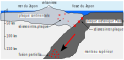
\includegraphics[scale=1]{../Figures_chap_intro/tectonik.pdf}
\caption[Schéma d'une zone de subduction]{Schéma de la zone de subduction de la fosse océanique du Japon. La subduction d'une plaque océanique donne naissance à des séismes, mais aussi à de nombreux phénomènes géophysiques comme le volcanisme à l'origine des reliefs de l'île du Japon (adapté de\,\cite{beig_friction_2006}).}
\label{fig:japon}
\end{figure}

\newpage

\minitoc
\newpage




\section{Les frottements solides}
\label{sec:frot}

\subsection{Que sont les frottements ?}

Les termes de \textit{frottement} ou de \textit{friction} désignent l'ensemble des interactions qui s'appliquent à deux systèmes mécaniques en contact et qui s'opposent à leur mouvement.
Le domaine de la physique qui étudie les frottements solides, la \textit{tribologie}, est définie comme la science de l'usure, des frottements et de la lubrification.
%Les phénomènes de frottement sont omniprésents tant dans notre quotidien que dans les applications technologiques de pointe ou les évènements géophysiques
Ces phénomènes sont omniprésents dans notre quotidien. Nous les retrouvons par exemple dans le simple fait de marcher, puisque c'est l'existence d'un frottement solide entre nos chaussures et le sol qui nous propulse en avant. Ceci est bien illustré par la grande difficulté avec laquelle
%\href{https://youtu.be/qQE-lMtGaN8}{\textcolor{black}{nous nous déplaçons sur la glace}},
nous nous déplaçons sur la glace,
surface à frottements faibles\,\cite{bowden_friction_1953}.


Cette section discute, par une approche historique, des mécanismes et modélisations du frottement solide. Ces mécanismes sont une première approche de la mécanique des failles, en particulier des séismes, qui peuvent être décrits comme la manifestation d'un mouvement de stick-slip, caractéristique des interfaces frictionnelles\,\cite{brace_stick-slip_1966}. 

\subsection{Origine microscopique des forces de frottement macroscopiques}

\begin{figure}[htb]
\centering
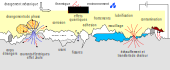
\includegraphics[scale=1]{../Figures_chap_intro/microscopic_complexity.pdf}
\caption[Complexité d'une interface réelle]{Visualisation schématique d'un contact frictionnel réel, et des interactions à l'œuvre à l'interface. L'aire de contact réelle entre les deux solides est nettement plus faible que l'aire de contact apparente.}
\label{fig:asperit}
\end{figure}




Lors d'un contact frictionnel entre deux objets, les frottements solides se manifestent à l'échelle macroscopique par l'apparition d'une force opposée à leur mouvement relatif. L'origine de cette force est à chercher à l'échelle microscopique. Une surface qui nous apparaît lisse au toucher est en réalité rugueuse, couverte d'aspérités dont la position et la taille sont aléatoires, à la manière d'un papier abrasif microscopique, allant selon les matériaux et traitements de surfaces du nanomètre au millimètre. Lors de la mise en contact de deux solides, ces aspérités s'entremêlent, répartissant la force pressante sur de multiples points de contacts, nommés \textit{microcontacts}. Ces points sont le siège d'un ensemble complexe d'interactions électrostatiques, chimiques et mécaniques, dans lesquelles interviennent les deux surfaces rugueuses des solides, mais également les impuretés et corps étrangers présents entres ceux-ci (Fig.\,\ref{fig:asperit}). La complexité de ces interactions rend irréaliste l'étude du comportement d'une interface rugueuse par le calcul exact de toutes les forces qui s'y exercent. L'étude de ces interfaces s'est donc historiquement faite au travers de lois empiriques macroscopiques telles que les lois d'Amontons-Coulomb (Sec.\,\ref{sec:coulomb}), puis par des lois justifiées par des modèles microscopiques des contacts à l'interface, comme le modèle de Bowden et Tabor, puis les modèles dits \textit{Rate-and-State} (Sec.\,\ref{sec:microfric}).

La prochaine section est dédiée aux premières tentatives de la modélisation de la friction solide par les lois d'Amontons-Coulomb.


\subsection{Description macroscopique -- Lois d'Amontons-Coulomb}
\label{sec:coulomb}


\begin{figure}[htb]
\centering
\includegraphics[width=.45\textwidth]{../Figures_chap_intro/vinci.png}
\caption[Croquis de Léonard de Vinci]{Croquis de Léonard de Vinci au sujet du frottement d'un objet sur une surface. Les dessins représentent des expériences d'étude de la friction par traction dans lesquelles différents objets sont tractés par une masse leur étant reliée par une cordelette et une poulie (adapté de\,\cite{hutchings_leonardo_2016}).}
\label{fig:vinci}
\end{figure}

Bien que les premiers écrits sur les frottements solides remontent à l'antiquité romaine, Thémistios écrivant notamment au quatrième siècle dans son \textit{De la Physique} «\,Il est plus facile d'entretenir le mouvement d'un corps se déplaçant que d'initier celui d'un corps au repos\,»\,\cite{themistius_aristotle_2008}, la première modélisation des frottements solides est due à Léonard de Vinci au XV\up{ème} siècle, dans son \textit{Codex Atlanticus} (Fig.\,\ref{fig:vinci})\,\cite{hutchings_leonardo_2016}. Ces travaux, redécouverts par Guillaume Amontons en 1699, et complétés par Leonhard Euler (1750) et Charles-Augustin de Coulomb (1785), ont abouti à la modélisation du problème à deux corps en contact frictionnel et à l'établissement de trois lois macroscopiques permettant de le résoudre.

\subsubsection{Définition du problème}

\begin{figure}[htb]
\centering
\includegraphics[scale=1]{../Figures_chap_intro/coulomb.pdf}
\caption[Référentiel utilisé pour les lois de Coulomb]{Définition du système étudié. Le référentiel choisi est celui du laboratoire muni d'un repère orthonormé direct $\left(\vec{e_x},\,\vec{e_y},\,\vec{e_z}\right)$. Le plan dans lequel le contact entre la masse et la surface s'effectue est le plan  $\left(\vec{e_x},\,\vec{e_z}\right)$, et $\vec{e_y}$ est pris orthogonal à ce plan, et orienté vers le haut (et de manière plus générale dans la direction opposée à la force pressante).
}
\label{fig:coulomb}
\end{figure}

Le système que nous considérons dans le cadre de la friction entre deux solides est une masse $m$ indéformable dont la surface macroscopiquement lisse d'aire $A$ est déposée sur un support horizontal immobile (Fig.\,\ref{fig:coulomb}). Sa vitesse est notée $\vec{v}$, et la direction de la vitesse $\vec{u_v} = \vec{v}/\norm{\vec{v}}$. Nous nommons \textit{force normale} $\vec{F_N}$, ou force pressante, la projection de la somme des forces appliquées à la masse sur le vecteur normal à l'interface, en excluant la réaction du support.

Les phénomènes de friction entrent en jeu lorsqu'une force tend à mettre en mouvement le solide, et a donc une composante tangentielle à l'interface. Ils se manifestent par l'apparition d'une force $\vec{F_f}$, qui s'applique dans le plan de l'interface, dans la direction contraire au sens de la mise en mouvement. Nous nommerons alors \textit{force cisaillante} $\vec{F_S}$ la projection de toutes les forces appliquées à la masse dans le plan de l'interface, à l'exception de cette force de réaction due aux frottements (Fig.\,\ref{fig:coulomb}).

Le problème étant ainsi défini, nous pouvons énoncer les trois lois d'Amontons-Coulomb décrivant la force de frottement $\vec{F_f}$ en fonction des forces normale $\vec{F_N}$ et cisaillante $\vec{F_S}$ appliquées à la masse $m$.


\subsubsection{Lois d'Amontons-Coulomb}

La modélisation du comportement d'une interface frictionnelle repose sur trois lois fondamentales, nommées d'après ceux qui les ont découvertes et rendues publiques, Guillaume Amontons (1699) et Charles-Augustin de Coulomb (1785).

\myparagraph{Lois du frottement statique -- \boldmath$\mu_s$}

La première loi d'Amontons affirme que pour mettre en mouvement la masse lorsqu'elle est immobile, il faut lui appliquer une force cisaillante telle que $F_S=\mu_sF_N$, où $\mu_s$ est une constante nommée \textit{coefficient de frottement statique}. Elle s'écrit

\begin{equation}
\text{tant que }{v}=0\qquad
\begin{aligned}\left\{
	\begin{split}
		\max F_f &= \mu_s F_N\\
		\vec{F_f} &= -\vec{F_S}\\
	\end{split}
	\right.
\end{aligned}
\end{equation}


La deuxième loi d'Amontons stipule que la force de frottement, notamment $\mu_s$, ne dépend pas de l'aire de contact apparente entre les deux solides.


\myparagraph{Loi du frottement dynamique -- \boldmath$\mu_d$}


La troisième loi de la friction, ou loi de Coulomb, précise qu'une fois que le solide est mis en mouvement relativement au support, la force de frottement qu'il subit est toujours opposée à la direction du mouvement et de norme constante, indépendante notamment de sa vitesse de glissement. Cette troisième loi nous permet de définir le \textit{coefficient de frottement dynamique} $\mu_d$ tel que

\begin{equation}
\vec{F_f} = - \mu_d F_N\,\vec{u_v}
\end{equation}


Une conséquence intéressante de cette loi est que la force de frottement est non-conservative, puisque son travail dépend du chemin suivi par l'objet sur lequel elle s'applique. Sur un chemin $\mathscr{C}$ de longueur $L_{\mathscr{C}}$,  à force normale constante, le travail $W_{\mathscr{C}}(\vec{F_f})$ vaut


\begin{equation}
W_{\mathscr{C}}(\vec{F_f})
= \int_{\mathscr{C}}\vec{F_f}\cdot\mathrm{d}\vec{u_v}
= -\mu_dF_N
\times \int_{\mathscr{C}}\vec{u_v}\cdot\mathrm{d}\vec{u_v} 
= -\mu_dF_NL_{\mathscr{C}}
\label{eq:dissip}
\end{equation}

Ce travail étant toujours négatif, la force de frottement dynamique fait toujours perdre au système de l'énergie. L'énergie perdue, dissipée en chaleur, est proportionnelle à la distance parcourue par l'objet.




\subsubsection{Variabilité des coefficients de frottement}

Émergeant des lois d'Amontons-Coulomb, $\mu_s$ et $\mu_d$ peuvent être considérés comme des grandeurs caractéristiques d'une interface entre deux matériaux donnés. Selon les conditions expérimentales (état de surface, lubrification, humidité ambiante, etc.) ces coefficients varient, mais à conditions expérimentales fixées il est possible de tabuler leurs valeurs (Fig.\ref{table:coef}). Cependant même en conditions expérimentales contrôlées, les coefficients varient d'un échantillon à un autre, et d'une expérience à l'autre, d'un facteur typiquement de l'ordre de 10\%, et leur utilisation nécessite un regard critique\,\cite{ben-david_static_2011, blau_significance_2001, czichos_multilaboratory_1987} (Fig.\,\ref{fig:disparite}). L'indépendance de $\mu_d$ de la vitesse de glissement notamment est une approximation dont les limites sont expérimentalement observées (Sec.\,\ref{sec:evolutionmacro}).


% Émergeant des lois d'Amontons-Coulomb, $\mu_s$ et $\mu_d$ sont souvent considérés comme des grandeurs caractéristiques d'une interface entre deux matériaux donnés. En réalité ils dépendent des conditions expérimentales dans lesquelles les deux matériaux sont frottés, en particulier de l'état de surface de ceux-ci, ou de la présence de corps étrangers. Ces variations donnent lieu à des tables de valeurs de coefficients de frottement entre différents matériaux et dans différentes conditions (Fig.\ref{table:coef}). Même en conditions contrôlées, ces coefficients sont très variables d'un échantillon à l'autre, et d'une expérience à l'autre, et leur utilisation nécessite un regard critique\,\cite{ben-david_static_2011, blau_significance_2001, czichos_multilaboratory_1987} (Fig.\,\ref{fig:disparite}). L'indépendance de $\mu_d$ de la vitesse de glissement notamment est une approximation dont les limites sont expérimentalement observées (Sec.\,\ref{sec:evolutionmacro}).

\begin{figure}[htb]
\centering
\begin{tabular}{ |p{4.5cm}||p{3cm}|p{3cm}|  }
 \hline
 \multicolumn{3}{|c|}{Coefficient de frottement statique} \\
 \hline
 \textbf{Matériau de la corde}& \textbf{Sèche} & \textbf{Humide} \\
 \hline
 Nylon         & 0.10 -- 0.12 &  0.12 -- 0.15\\
 Polyester     & 0.12 -- 0.15 &  0.15 -- 0.17\\
 Polypropylène & 0.08 -- 0.11 &  0.08 -- 0.11\\
 Aramide        & 0.12 -- 0.15 &  0.15 -- 0.17\\
 HMPE          & 0.08 -- 0.11 &  0.08 -- 0.11\\
 \hline
\end{tabular}
\caption[Exemple de table de coefficients de frottement statique]{Exemple de table de coefficients de frottement statique. Sont tabulés ici les coefficients de frottement entre une plaque d'acier lisse et des cordes de différents matériaux, sèches ou humides\,\cite{mckenna_properties_2004}.}
\label{table:coef}
\end{figure}

\begin{figure}[htb]
\centering
\includegraphics[width=.6\textwidth]{../Figures_chap_intro/multilab.png}
\caption[Variabilité du coefficient de frottement]{Coefficients de frottement dynamique mesurés par différentes équipes de recherche sur des échantillons identiques en acier. Chaque point représente une expérience, et chaque colonne de points l'ensemble des résultats d'un laboratoire (extrait de\,\cite{ czichos_multilaboratory_1987}). Moyenne : $0.6$, écart type : $0.109$.}
\label{fig:disparite}
\end{figure}




\subsubsection{Émergence du phénomène de stick-slip}
\label{sec:ss1}

\begin{figure}[htb]
\centering
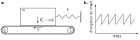
\includegraphics[scale=1]{../Figures_chap_intro/stickslip.pdf}
\caption[Mouvement de stick-slip sur un tapis roulant]{\textbf{a.} Système mécanique pouvant aboutir à un mouvement de stick-slip. \textbf{b.} Évolution temporelle typique de la longueur du ressort dans ce système. Les axes sont en unités arbitraires, de tels mouvements pouvant se produire à des échelles très variées.}
\label{fig:shemastickslip}
\end{figure}

Le phénomène de stick-slip, ou collé-glissé, est un mouvement saccadé entre deux solides liés par une interface frictionnelle, qui émerge de la différence entre $\mu_s$ et $\mu_d$.
Pour le mettre en évidence, considérons un système modèle composé d'une masse $m$, reliée à un support immobile par un ressort idéal de raideur $k$, et placée sur un tapis roulant évoluant à vitesse constante $v$ (Fig.\,\ref{fig:shemastickslip}). Alors si $\mu_d<\mu_s$, le mouvement se décompose en deux phases qui alternent :

\begin{itemize}
\bitem \textit{Stick} : les deux solides sont solidaires, leur mouvement relatif est nul, les lois d'Amontons décrivent les interactions frictionnelles entre les deux par le biais du coefficient de frottement statique $\mu_s$. Durant cette phase, l'interface se charge en cisaillement par les déformations du ressort.
\bitem \textit{Slip} : les deux solides se mettent en mouvement relatif, ils glissent, la troisième loi de Coulomb décrit le mouvement par le coefficient $\mu_d$.
\end{itemize}


Les lois d'Amontons Coulomb permettent d'aboutir à la description d'un mouvement périodique, de période $T_{ss}$,  et d'amplitude $A_{ss}$, qui en posant $\omega_0 = \sqrt{{k}/{m}}$ s'écrivent


\begin{align}[left=\empheqlbrace]
	\begin{split}
		T_{ss} &= 2\frac{(\mu_s-\mu_d) \,g}{\omega_0^2\,v} + \dfrac{\pi}{\omega_0}\\
		A_{ss} &= \frac{(\mu_s-\mu_d)\,g}{\omega_0 ^2}
	\end{split}
\label{eq:freqss}
\end{align}



Les lois d'Amontons-Coulomb permettent de décrire synthétiquement de nombreux systèmes frictionnels, mais sont limitées en raison des variations des coefficients de frottement en fonction du temps et de la vitesse, et de l'hétérogénéité des interfaces réelles. Elles ont été énoncées à leur origine sans justification microscopique, et relèvent d'une description empirique d'interfaces macroscopiques. Un modèle microscopique historiquement utilisé pour les décrire est détaillé dans la section suivante.



\subsection{Modèles microscopiques de la friction}

\label{sec:microfric}



La description par des modèles macroscopiques du frottement entre deux solides s'appuie historiquement sur des observations empiriques. Les modèles microscopiques justifiant de la validité des trois lois d'Amontons-Coulomb sont récents (\textsc{xx}\up{ème} siècle), avec notamment le modèle de Bowden et Tabor\,\cite{bowden_friction_1950}, publié en 1950. Ces modèles reposent sur la prise en compte de la réalité microscopique des contacts entre les deux solides.


\subsubsection{Description de l'aire de contact réelle}

\begin{figure}[h]
\centering	
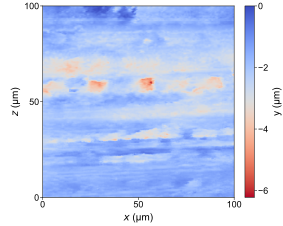
\includegraphics[scale=1]{../Figures_chap_intro/profiloplot_zoom.pdf}
\caption[Profil microscopique d'un bloc de PMMA]{Profil d'altitude d'une portion de bloc de plastique poli  à l'aide de papier abrasif fin (P1200). L'altitude de référence est la surface macroscopique du bloc. Les aspérités, dont la hauteur est de l'ordre de quelques micromètres, semblent aléatoirement distribuées. Cet échantillon présente des traces d'usure, sous la forme de rainures le long de l'axe $x$.}
\label{fig:asperit2}
\end{figure}


Lorsque deux solides sont en contact, l'aire de contact réelle entre les microaspérités à l'interface est bien plus faible que l'aire apparente macroscopique de contact $A$ (Fig.\,\ref{fig:asperit2}). Lors de la mise en contact de deux solides, seules les plus hautes aspérités de chaque surface se rencontrent. L'aire réelle de contact est nommée $A_r$ et peut être décrite comme la somme des aires de chaque aspérité en contact. Cette aire est par exemple mesurable dans les solides transparents par des méthodes optiques reposant sur la réflexion interne totale de la lumière\,\cite{dieterich_direct_1994}.
Afin de modéliser le contact entre les deux solides, un modèle du comportement des microcontacts soumis à une pression et de leur distribution est nécessaire.

La mécanique des contacts est un domaine de recherche riche et actif, et nous n'en proposons dans ce chapitre qu'un aperçu, au travers de deux modèles historiques de contacts uniques. Il  existe cependant d'autres méthodes pour aborder ce type de problèmes, plus récentes et plus précises\,\cite{greenwood_contact_1966, derjaguin_effect_1975,  johnson_surface_1971, maugis_adhesion_1992, persson_theory_2001, vakis_modeling_2018}, que nous n'aborderons pas ici.




Dans cette section, de façon à distinguer les forces macroscopiques $F_N$ et $F_S$ des forces à l'échelle des microcontacts, nous nommerons en minuscule $f_n$ et $f_s$ les forces appliquées sur un microcontact de surface $A_\mu$, de telle sorte qu'une contrainte $\sigma$ subie par ce microcontact s'écrive $\sigma=f/A_\mu$.


\subsubsection{Modèles d'aspérités}




Nous présentons deux modèles d'aspérités sans adhésion, selon que la pression de contact est faible, et les déformations élastiques, ou que la pression est forte, et les déformations plastiques.

\myparagraph{Aspérité élastique}

Pour une aspérité individuelle élastique, de module d'Young $E$ et de coefficient de Poisson $\nu$, nous noterons $E^*={E}/(1-\nu^2)$. Dans le cadre du contact de Hertz\,\cite{hertz_ueber_1882}, si cette aspérité dispose d'un rayon de courbure $\rho_r$ et est pressée contre une surface dure sous une force normale $f_n$, alors son aire de contact avec cette surface est

\begin{equation}
A_\mu = \pi\left(\frac{3}{4}\times\frac{1}{E^*}\times\rho_r\times f_n\right)^{2/3}\propto f_n^{2/3}
\end{equation}



Ainsi l'aire de contact augmente proportionnellement à $f_n^{2/3}$, tandis que la pression subie par le contact, $f_n/A_\mu$, augmente proportionnellement à $f_n^{1/3}$.


\myparagraph{Aspérité plastique}

\begin{figure}[htb]
\centering
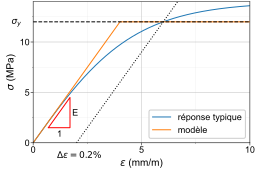
\includegraphics[scale=1]{../Figures_chap_intro/yield.pdf}
\caption[Limite de plasticité d'un matériau]{Réponse contrainte-déformation d'un matériau plastique typique, avec $E=\SI{3}{\giga\pascal}$ et $\sigma_Y=\SI{12}{\mega\pascal}$. En bleu, exemple de réponse typique du matériau. Dans les régimes que nous considérons, la contrainte est une fonction croissante de la déformation. Nous la modélisons par la courbe orange. Ce modèle comporte d'abord une réponse purement élastique, telle que si $\varepsilon<\sigma_Y/E$ alors $\sigma=E\varepsilon$, puis une réponse purement plastique, telle que si $\varepsilon\geq\sigma_Y/E$, alors $\sigma = \sigma_Y$. La définition communément acceptée de $\sigma_Y$, représentée par les lignes pointillées, est la valeur de contrainte telle qu'une fois le matériau de nouveau déchargé, sa déformation plastique soit de 0.2\%\,\cite{avallone_marks_2006}.}
\label{fig:yield}
\end{figure}




Si les contraintes subies par les microcontacts sont grandes les déformations sont plastiques, et $\sigma$ atteint un maximum. La contrainte limite d'élasticité $\sigma_Y$ (\textit{yield stress}, homogène à une pression) est définie comme la contrainte à partir de laquelle les déformations de l'aspérité deviennent plastiques (Fig.\,\ref{fig:yield}). La valeur de $\sigma_Y$ est une caractéristique du matériau. Les valeurs typiques de $\sigma_Y$ sont de l'ordre de quelques $10^7\,\text{Pa}$ pour la plupart des matériaux polymères rigides\,\cite{avallone_marks_2006}. Cela correspond environ à dix fois la contrainte normale que nous appliquons sur la surface \textit{apparente} de nos échantillons expérimentaux (Sec.\,\ref{sec:echantillons}).

Si une force normale $f_n$ est appliquée sur un microcontact plastique de surface de contact $A_{\mu}$, celle-ci ne pouvant supporter qu'une contrainte normale $\sigma_n=\sigma_Y$, alors

\begin{equation}
A_\mu = \frac{f_n}{\sigma_Y}
\label{eq:microcontact}
\end{equation}

Ainsi, $A_\mu$ augmente linéairement avec $f_n$.


\myparagraph{Cisaillement d'une aspérité}

Qu'il soit élastique ou plastique, un microcontact résiste au glissement tant qu'il n'est pas brisé ou affaibli. Sa résistance au cisaillement $\sigma_r$ correspond à la contrainte cisaillante maximale qu'il peut supporter sans glisser. La force cisaillante $f_s$ maximum que le microcontact peut retenir est donc

\begin{equation}
\max f_s = A_\mu\times \sigma_r
\end{equation}

Ainsi la force cisaillante maximale que peut supporter un microcontact avant de glisser augmente linéairement avec $A_\mu$.

\pagebreak

En conclusion, ces deux modèles montrent que la surface d'un microcontact augmente avec la force normale qu'il porte. Elle est proportionnelle à la force normale dans le cas d'un microcontact plastique, tandis que pour un microcontact élastique elle est proportionnelle à $f_n^{2/3}$. La force cisaillante que peut retenir un microcontact est pour sa part proportionnelle à cette surface. Ces modèles de microcontacts peuvent maintenant être appliqués à l'échelle d'une interface toute entière.




\subsubsection[Modèle d'interface -- lois d'Amontons-Coulomb]{Modèle d'interface -- justification des lois d'Amontons-Coulomb}
\label{sec:amontonsmicro}

Nous restreignons cette présentation au cas d'une interface dont les contacts ont un comportement plastique car les matériaux que nous étudions dans les conditions choisies sont correctement décrits par ce modèle\,\cite{rubinstein_crack-like_2006}. Cependant les résultats présentés resteraient valides pour une interface partiellement ou entièrement élastique avec une distribution gaussienne des hauteurs des aspérités\,\cite{singer_contact_1992}.

\myparagraph{Frottement statique}

Dans le cas d'une interface plastique, le modèle de Bowden et Tabor\,\cite{bowden_friction_1950} décrit la surface comme un ensemble de microcontacts de surfaces $\{A_{\mu,i}\}_i$. La force normale portée par l'interface peut alors s'écrire comme la somme des forces normales portées par l'ensemble des microcontacts, $F_N = \sum_if_{n,i}$. En appliquant l'Équation\:\ref{eq:microcontact} à chacun de ces microcontacts nous obtenons

\begin{equation}
A_r = \sum_i A_{\mu,i} = \sum_i\frac{f_{n,i}}{\sigma_Y} = \frac{F_N}{\sigma_Y}
\label{eq:wamu}
\end{equation}

Ainsi l'aire de contact réelle $A_r$ de l'interface est proportionnelle à la force normale $F_N$ qui lui est appliquée. En appliquant un raisonnement similaire sur la force cisaillante, répartie sur tous les microcontacts, nous obtenons $\max F_S = \sum_i \max f_{s,i} = \sum_i  \sigma_rA_{\mu,i} = \sigma_r A_r$. Ainsi le coefficient de frottement statique se définit comme

\begin{equation}
\max F_S = \mu_sF_N\qquad\text{avec} \qquad \mu_s = \dfrac{\sigma_r}{\sigma_Y}
\label{eq:maxfs1}
\end{equation}



Au travers cette modélisation microscopique nous retrouvons les deux lois d'Amontons, ainsi qu'une définition du coefficient de frottement statique. Cette définition reste sujette à discussion, puisqu'elle repose sur l'utilisation de $\sigma_Y$ et $\sigma_r$. La contrainte limite d'élasticité $\sigma_Y$ est une caractéristique du matériau, et la considérer constante est une bonne approximation. La résistance au cisaillement $\sigma_r$ pour sa part n'est pas une grandeur caractéristique. Elle dépend de la géométrie des contacts et de chaque aspérité considérée, et n'est pas à priori connue.


\myparagraph{Frottement dynamique}


Lorsque l'interface est en glissement quasi-statique, les microcontacts se cassent et se reforment de manière répétée. La formation d'un point de contact s'accompagne de l'accumulation rapide de contraintes cisaillantes sur ce point, puis à une nouvelle mise en glissement. Les deux aspérités poursuivent leur glissement jusqu'à rencontrer une nouvelle aspérité avec laquelle répéter ce cycle. Tandis que le solide glisse de manière quasi-statique, les microcontacts subissent des mouvements rapides et irréguliers\,\cite{persson_sliding_1998,beig_friction_2006}. En reprenant la description du contact unique cisaillé proposée plus haut (Éq.\,\ref{eq:wamu} et\,\ref{eq:maxfs1}), chaque rupture de microcontact s'effectue à une force cisaillante $f_s$ telle que

\begin{equation}
f_s=A_\mu\times\sigma_r= \dfrac{\sigma_r}{\sigma_Y}f_n
\end{equation}

Ainsi, peu importe la vitesse à laquelle le glissement est effectué, si nous considérons comme isotrope la répartition des microcontacts, la force cisaillante macroscopique $F_S$ est de valeur constante

\begin{equation}
F_S = \mu_dF_N\qquad\text{avec} \qquad \mu_d = \mu_s = \dfrac{\sigma_r}{\sigma_Y}
\label{eq:maxfs}
\end{equation}


Les limitations de ce modèle sont ainsi mises en exergue, puisqu'il ne parvient pas à prédire de différence entre $\mu_s$ et $\mu_d$, ni l'évolution de ces deux coefficients en fonction du temps et de la vitesse de glissement observée expérimentalement pour des interfaces solide-solide réelles.



\subsection[Modélisation de l'évolution de $\mu$]{Modélisation de l'évolution des coefficients de frottement}
\label{sec:evolutionmacro}

Les coefficients de frottement ne sont pas des caractéristiques d'une interface, comme décrit précédemment. Le coefficient de frottement statique tend à augmenter avec l'âge de l'interface, tandis que le coefficient de frottement dynamique, à l'inverse de ce que stipule la troisième loi de Coulomb, dépend de la vitesse de glissement. Cette section décrit ces observations et un modèle empirique permettant d'en rendre compte.

\subsubsection{Vieillissement d'une interface au repos}
\label{sec:aging}

\begin{figure}[htb]
\centering
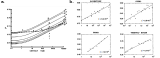
\includegraphics[scale=1]{../Figures_chap_intro/aging.pdf}
\caption[Vieillissement d'une interface bloquée]{\textbf{a.} Évolution du coefficient de frottement statique $\mu$ en fonction du temps de contact normalisé ($\tau=\theta/\theta_0$) pour différentes roches (extrait de\,\cite{dieterich_modeling_1979}). Les échantillons étudiés sont des granodiorites californiennes poncées avec des papiers abrasifs P60 à P600. Pour tous les échantillons présentés, le coefficient augmente proportionnellement au logarithme de l'âge de l'interface. \textbf{b.} Évolution du coefficient de frottement statique $\mu_s$ en fonction du temps de contact $\tau$ dans divers matériaux (extrait de\,\cite{baumberger_contact_1997}). La ligne est un ajustement des points de la forme $\mu(\tau)=\mu_0+\text{b}\ln\tau$.}
\label{fig:aging}
\end{figure}



Le coefficient de frottement statique augmente logarithmiquement avec le temps de contact entre les deux solides (Fig.\,\ref{fig:aging}), dans tous les matériaux, y compris les roches et les matières plastiques\,\cite{dieterich_modeling_1979,baumberger_contact_1997} comme le polyméthacrylate de méthyle (PMMA) que nous utilisons dans nos expériences (Sec.\,\ref{sec:materials}). Ce vieillissement (\textit{aging}) s'explique par une augmentation logarithmique de la surface réelle de contact $A_r$. Le mécanisme sous-jacent est que les microcontacts, de part leur échelle microscopique, s’étalent avec le temps sous l'effet de l'agitation thermique. Telles des particules dans un potentiel comportant des minima locaux, lorsque ces aspérités sont soumises à des fluctuations thermiques, elles sautent de minimum en minimum, augmentant progressivement l'aire de contact réelle entre les deux surfaces. Ce phénomène est nommé \textit{fluage} (\textit{indentation creep})\,\cite{cocks_indentation_1991,dieterich_direct_1994,baumberger_solid_2006}.



\subsubsection[Influence de la vitesse sur $\mu$]{Influence de la vitesse sur le coefficient de frottement}

\begin{figure}[htb]
\centering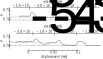
\includegraphics[scale=1]{../Figures_chap_intro/speed_mu.pdf}
\caption[Évolution de $\mu$ lors d'un saut de vitesse]{Évolution du coefficient de frottement dynamique en fonction de la vitesse (adapté de\,\cite{dieterich_modeling_1979}). Les échantillons étudiés sont des granodiorites d'une carrière californienne poncées avec du papier abrasif. La vitesse de déplacement varie au cours de l'expérience.}
\label{fig:speed_mu}
\end{figure}





Lorsqu'un solide est en glissement sur une surface, son coefficient de frottement évolue en fonction de la vitesse de glissement $V$ (Fig.\,\ref{fig:speed_mu}). En régime de glissement stable, $\mu$ est proportionnel au logarithme de  $V$\,\cite{ruina_slip_1983,stesky_mechanisms_1978,blanpied_frictional_1987,dieterich_direct_1994}. Lors d'un saut de vitesse positif, à temps court, $\mu$ augmente, puis relaxe à temps long vers une nouvelle valeur stable. Ce comportement provient de la concurrence de deux effets. L'augmentation initiale de $\mu$ est l'effet de la résistance intrinsèque des contacts\,\cite{dieterich_direct_1994}. La diminution qui s'en suit relève d'un mécanisme de fluage similaire à celui à l'œuvre dans le vieillissement d'une interface au repos.
L'interface est le siège d'une compétition entre le renouvellement des contacts par son glissement et le vieillissement des contacts sous une charge normale.
%Plus la vitesse est élevée, moins les contacts nouvellement formés ont le temps de vieillir avant d'être à nouveau brisés.


Ces deux dépendances logarithmiques de $\mu$ en temps et en vitesse peuvent être décrites par des loi empiriques telles que celle proposée par Dieterich et Ruina en 1979 et 1983, que nous présentons ci-dessous.

\subsubsection{Modèle de Dieterich et Ruina -- Rate-and-State}
\label{sec:rateandstate}


\begin{figure}[h!]
\centering
\includegraphics[scale=1]{../Figures_chap_intro/velocity_s_w.pdf}
\caption[Comportement du modèle Rate-and-State]{Schéma du comportement d'un système frictionnel suivant une loi Rate-and-State, en fonction des paramètres $A$ et $B$ du modèle (adapté de\,\cite{zhang_frictional_2022}). La courbe rouge (resp. bleue) présente une friction renforcée (resp. affaiblie) par la vitesse.}
\label{fig:velocity_s_w}
\end{figure}

\newpage

Le modèle de Dieterich et Ruina\,\cite{dieterich_modeling_1979,ruina_slip_1983} est un modèle \textit{Rate-and-State} (\textit{taux-état}, rarement traduit dans la littérature), reliant le coefficient de frottement $\mu$ à la vitesse de glissement $V$ et à une fonction d'état $\theta$, selon l'équation 

\begin{equation}
\mu = \mu_0+A\ln\left(1+\frac{V}{V_0}\right)+B\ln\left(1+\frac{\theta}{\theta_0}\right)
\end{equation}


La loi décrite ici étant empirique, son interprétation physique est sujette à des réserves\,\cite{dieterich_direct_1994}. Il est cependant possible d'en trouver des justifications microscopiques\,\cite{baumberger_physical_1999, nakatani_conceptual_2001,chen_microphysically_2017}. Ainsi $\theta$ est généralement interprété comme l'âge des microcontacts formés entre les deux solides. Les constantes $\theta_0$, $\mu_0$ et $V_0$ sont déterminées expérimentalement.

Cette équation doit être couplée avec une équation d'état modèle pour l'évolution de $\theta$. L'équation proposée par Dieterich considère que l'âge des contacts évolue selon l'équation

\begin{equation}
\diff{\theta}{t} = 1-\frac{\theta V}{D_c}
\end{equation}

La constante $D_c$, homogène à une longueur, correspond à la distance de glissement caractéristique nécessaire pour renouveler entièrement une population de contacts. Ce modèle permet d'exprimer à vitesse nulle le coefficient de frottement statique et de rendre compte de son augmentation logarithmique avec le temps.

\begin{equation}
\mu_s=\mu_0+B\ln(1+\theta/\theta_0)
\end{equation}

Lorsque le glissement se fait en régime stationnaire, $V$ est constante et $\theta = D_c/V$. Nous considérons les cas où $V/V_0\gg1$ et $D_c/V\theta_0\gg1$, hypothèses généralement valides pour les systèmes que nous étudions. Le cas général ainsi que les limites inverses de ces hypothèses sont traités dans la littérature\,\cite{bar-sinai_slow_2012, barsinai_velocitystrengthening_2014,bar-sinai_velocity-strengthening_2015}. Nous obtenons alors


\begin{equation}
\mu = \text{const.}+(A-B)\ln(V)
\end{equation}


Ce modèle met en évidence deux constantes $A$ et $B$, représentant respectivement la résistance au cisaillement des contacts et celle du vieillissement statique. L'effet de $A$, nommé \textit{effet direct}, est visible à temps court et va toujours dans le sens de la résistance au changement de vitesse. L'effet de $B$, ou \textit{effet indirect}, est visible à temps longs, lorsque le glissement est supérieur à $D_c$ (Fig.\,\ref{fig:velocity_s_w}). Lorsque le vieillissement est dominant, $B>A$, le frottement est d'autant plus faible que la vitesse est grande, il est dit affaibli par la vitesse (\textit{velocity weakening}). Dans le cas inverse, $A>B$, le frottement est renforcé par la vitesse (\textit{velocity strengthening}).

Ce modèle, bien que justifié par des considérations microscopiques, reste empirique. Aussi d'autres lois d'évolution de $\theta$ existent, représentant plus fidèlement le comportement de l'interface lorsqu'elle est soumise à des variations rapides de vitesse. Toutes cependant permettent de rendre compte d'un écart entre $\mu_s$ et $\mu_d$, et de l'apparition de deux régimes de déplacement, le glissement stable et le stick-slip\,\cite{ruina_slip_1983,nagata_revised_2012,aharonov_physicsbased_2018}.


\subsubsection{Instabilité de stick-slip}


\begin{figure}[htb]
\centering
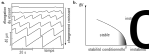
\includegraphics[scale=1]{../Figures_chap_intro/stability.pdf}
\caption[Diagramme de stabilité d'un mouvement de stick-slip]{\textbf{a.} Réponse d'un système masse-ressort posé sur un tapis roulant à vitesse constante. Lorsque la force normale décroît, le comportement de la masse effectue une transition entre un régime de stick-slip et un glissement permanent à vitesse variable, puis un glissement stable (adapté de\,\cite{baumberger_physical_1999}). \textbf{b.} Diagramme de stabilité schématique d'une interface affaiblie par la vitesse (adapté de \,\cite{scholz_earthquakes_1998}). Ce diagramme montre le saut de vitesse nécessaire afin de déstabiliser une interface en glissement stable, en fonction de la contrainte normale qui lui est appliquée. Le régime instable évolue en stick-slip quel que soit la perturbation de vitesse, tandis que le régime de stabilité conditionnelle n'évolue en stick-slip que si le saut de vitesse est suffisant.}
\label{fig:ss2}
\end{figure}


Dans le cas d'une interface à frottement renforcé par la vitesse, un mouvement de glissement est intrinsèquement stable. Une fluctuation de vitesse se traduit par un changement de vitesse de glissement stable. Une interface à frottement affaibli par la vitesse en revanche peut exhiber un comportement instable de stick-slip, comme conséquence de l'existence d'un coefficient de frottement dynamique inférieur au coefficient de frottement statique (Sec.\,\ref{sec:ss1}, Fig.\,\ref{fig:ss2}a). Ce comportement instable en vitesse est bien décrit par une bifurcation de Hopf\,\cite{rice_stability_1983,gu_slip_1984,heslot_creep_1994}. Si l'on considère un écart de vitesse $\Delta V$ appliqué à une interface en glissement stable, et $\sigma$ la pression normale appliquée sur l'aire de contact apparente $A$, il est possible de définir une valeur critique $\sigma_c$ de cette pression à laquelle le comportement du système passe d'un régime toujours instable à un régime conditionnellement stable (Fig\,\ref{fig:ss2}b).


Cette analyse de stabilité met en avant l'existence d'interfaces toujours en glissement stable car renforcées par la vitesse, et d'interfaces toujours instables car affaiblies par la vitesse et dans la zone instable du diagramme de bifurcation. Le modèle prédit également l'existence d'interfaces affaiblies par la vitesse, conditionnellement stables, nécessitant une fluctuation de vitesse pour entrer dans un régime de stick-slip. Cette fluctuation peut consister en la rupture partielle d'une interface, la portion instable de celle-ci entraînant une déstabilisation de sa portion conditionnellement stable. La détermination du caractère renforcé ou affaibli par la vitesse des portions de failles est à ce titre un enjeu majeur de l'étude des failles.




Le modèle Rate-and-State, couplé à une équation d'état, permet une bonne description de la dynamique d'une interface frictionnelle. Sa principale limitation réside dans son aspect empirique, nécessitant des ajustements pour déterminer les constantes $A$ et $B$ pour chaque système étudié. Dans un système de failles réelles, la connaissance des phénomènes à l'origine de leurs variations est nécessaire à l'étude et la prévision de la stabilité du mouvement. De plus les modèles présentés ne décrivent que le mouvement moyen de l'interface, celui du centre de masse du système, et ignorent son extension spatiale.

Cette dernière problématique soulève la question du mécanisme par lequel le mouvement s'initie. En effet cette initiation n'étant pas instantanée, elle doit s'accompagner d'un phénomène propagatif. Ce phénomène est la propagation d'une rupture interfaciale affaiblissant de proche en proche les microcontacts et permettant la mise en glissement de l'interface.



\newpage

\section{Mécanique de la fracture linéaire élastique}
\label{sec:LEFM}

Nous avons présenté dans la section précédente qu'une interface frictionnelle entre deux solides possède une structure complexe, étudiée au travers de modèles empiriques macroscopiques, justifiés par des considérations microscopiques. Ces modèles comme celui de Bowden et Tabor ou de Dieterich et Ruina font état de la réalité des contacts microscopiques à l'interface, mettant notamment en évidence la différence entre l' entre l'aire de contact réelle $A_r$ et l'aire de contact macroscopique $A$ aire de contact réelle $A_r$ et l'aire de contact macroscopique $A$ entre les deux solides. Ils ne fournissent cependant qu'un modèle pour le déplacement moyen des blocs à l'interface. 
%sur l'approximation que les solides en contact se déplacent %d'un bloc, sans déformations internes, comme infiniment rigides.
L'élasticité responsable de leur mouvement de stick-slip est alors extérieure au système, modélisable par un ressort effectif relié à une masse indéformable en frottement sur une surface fixe.
Dans la réalité pourtant l'élasticité provient des blocs en frottement eux-mêmes. Ils sont élastiques et se déforment, y compris à proximité de l'interface. Le changement brutal de vitesse lors d'une phase de slip n'est en réalité pas instantané. Tous les microcontacts n'entrent pas en glissement simultanément, mais s'affaiblissent de proche en proche au cours d'un phénomène propagatif, un \textit{crack} ou \textit{fracture}, ou encore \textit{rupture}.

La propagation de cette fracture s'accompagne de la libération dans le matériau d'ondes de compression et de cisaillement se propageant jusqu'en surface, et qui dans le cas des failles sismiques donnent naissance à un séisme. Cette rupture engendre une chute de contrainte cisaillante locale, et se déplace à des vitesses pouvant atteindre la vitesse du son dans le milieu. Elle correspond à une fracture en mode de cisaillement, décrite par la mécanique de la fracture linéaire élastique (LEFM, pour \textit{Linear Elastic Fracture Mechanics})\,\cite{svetlizky_brittle_2019}.


Dans cette section, nous présentons les principes de la propagation de fractures dans les matériaux et leur application à l'étude des frottements solides. La première partie décrit les bases de la théorie de l'élasticité que nous allons utiliser par la suite, la deuxième les fondements de la fracture statique puis dynamique, dont la théorie de Griffith, et la troisième l'application de la mécanique de la fracture linéaire élastique à la propagation de ruptures le long des interfaces frictionnelles.





\subsection{Mécanique du solide élastique}
\label{sec:hook}
La mécanique du solide élastique est le domaine de la physique qui décrit le comportement d'un objet solide ayant une réponse élastique linéaire lorsqu'il est soumis à des contraintes extérieures. Nous rappelons brièvement dans cette section la loi de Hooke régissant la réponse d'un solide élastique à une contrainte extérieure.

%\subsubsection{Loi de Hooke pour un ressort}


\begin{figure}[htb]
\centering
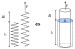
\includegraphics[scale=1]{../Figures_chap_intro/hooke.pdf}
\caption[Loi de Hooke pour un ressort]{Déformations d'un solide induites par une force extérieure. Tout solide élastique se comporte comme un ressort dont la raideur dépend de son module d'Young $E$ et de sa géométrie.}
\end{figure}


\newpage
%
%Lorsqu'un ressort idéal de longueur $l$ est soumis à une force de traction ou de compression, celui-ci se déforme, et produit une force $\vec{F}$ dans la direction opposée à la déformation en retour. Cette force est proportionnelle à l'étirement du ressort $\Delta l$, selon un coefficient de raideur $k$ de telle sorte que
%
%\begin{equation}
%F=-k\Delta l
%\end{equation}
%
%Le modèle du ressort décrit une pièce mécanique idéalisée, que l'on ne déformerait que selon un seul axe, et qui n'aurait qu'une seule dimension. Cette pièce se comporte alors comme un ressort, dont la longueur et la raideur sont déterminées par les propriétés du matériau qui la compose et sa géométrie. La loi de Hooke est une généralisation de la loi des ressors pour un solide.
%

\subsubsection{Loi de Hooke uniaxiale pour un solide élastique}

\myparagraph{Module d'Young}

%La géométrie d'une pièce mécanique est un facteur déterminant de sa réponse aux contraintes extérieures.
Lorsqu'une pièce mécanique est soumise à une force extérieure, l'étirement total qu'elle subit dépend de sa géométrie. À force égale, une barre deux fois plus longue s'allonge deux fois plus, tandis que la même force appliquée sur une surface deux fois plus grande l'allonge deux fois moins. Afin d'éliminer ces considérations, nous utilisons la contrainte $\sigma=F/A$ définie comme le rapport de la force $F$ appliquée sur la surface $A$, et l'allongement relatif, ou déformation, $\varepsilon=\Delta l/l_0$ défini comme le rapport entre l'allongement de la pièce $\Delta l$ et sa longueur à vide $l_0$. La \textit{loi de Hooke}\,\cite{hooke_potentia_1674} stipule alors qu'il existe un coefficient $E$ nommé \textit{module d'Young} tel que

\begin{equation}
\sigma=E\varepsilon
\end{equation}

Cette pièce se comporte alors comme un ressort, dont la raideur est déterminée par les propriétés du matériau qui la compose, sa longueur et sa géométrie. La loi de Hooke est une généralisation de la loi des ressorts pour un solide. Le module d'Young s'exprime en pascals. Pour le PMMA, matériau que nous utilisons dans cette étude, $E_{PMMA}\sim\SI{3}{\giga\pascal}$.
%et sa valeur varie typiquement du mégapascal pour les matériaux tels que le caoutchouc à plusieurs centaines de gigapascals pour les métaux\,\cite{feynman_feynman_1963}.

\myparagraph{Coefficient de Poisson}

La pièce raccourcie ou allongée sous l'effet de la contrainte voit également sa largeur changer. Lorsqu'un matériau est soumis à une contrainte $\sigma_\parallel$ selon un axe, il subit une déformation $\varepsilon_{\parallel} =\sigma_{\parallel} /E$ selon cet axe, mais également une déformation $\varepsilon_\perp$ dans le plan orthogonal à cet axe. Le \textit{coefficient de Poisson} est alors défini comme


\begin{equation}
\nu = -\frac{\varepsilon_\perp}{\varepsilon_{\parallel} }
\end{equation}


Le coefficient de Poisson est sans unité. Il prend des valeurs entre 0 et 0.5 et varie typiquement de 0.1 à 0.4 dans la plupart des matériaux courants\,\cite{feynman_feynman_1963}.

\subsubsection{Loi de Hooke généralisée}

Si l'on s'intéresse maintenant à une contrainte non unidirectionnelle, les contributions des contraintes s'additionnent. Il nous faut considérer le cas d'un petit cube de matière infinitésimal soumis à des contraintes, exprimées sous la forme d'un tenseur $[\sigma] = [\sigma_{i,j}]_{i,j\in\{1,2,3\}}$, où 1, 2 et 3 représentent les trois directions d'un repère orthonormé. Il en va de même pour $[\varepsilon]$. Sous l'hypothèse que le matériau est homogène et isotrope, toujours vérifiée par la suite, la loi de Hooke se généralise\,\cite{feynman_feynman_1963} sous la forme

\begin{equation}
[\sigma] = \frac{E}{1+\nu }\left( [\varepsilon] +\frac{\nu }{1-2\nu }\operatorname{Tr}\left( [\varepsilon] \right) \mathbf I_3 \right) 
\end{equation}

Soit encore en convention de sommation d'Einstein

\begin{equation}
\sigma_{ij} = \frac{E}{1+\nu } \left( \varepsilon_{ij}+\frac{\nu }{1-2\nu }\varepsilon_{kk} \delta _{ij}\right)
\end{equation}


Ainsi nous disposons d'une relation close permettant de lier les déformations aux contraintes subies par un matériau. Couplées à des conditions aux limites et des informations sur la géométrie des pièces considérées, cette équation nous permet de résoudre entièrement le problème de la répartition des contraintes. Dans notre étude nous utilisons des pièces dont la forme est celle de plaques minces, qui nous permettent de considérer un système 2D à trois degrés de liberté.


\subsubsection{Cas des plaques}

Une \textit{plaque} est une pièce dont la forme est celle d'un parallélépipède dont une des dimensions, notée $z$, est beaucoup plus faible que les autres. Sous la condition que la pièce est une plaque mince, nous pouvons effectuer l'hypothèse dite de \textit{planéité des contraintes} (\textit{plane stress}), qui considère que les contraintes appliquées selon l'axe $z$ sont toutes nulles, c'est à dire que $\sigma_{xz}=\sigma_{yz}=\sigma_{zz}=0$. Sous cette hypothèse la loi de Hooke se réécrit\,\cite{freund_dynamic_1990}


\begin{equation}
\begin{pmatrix}
\sigma_{xx} \\
\sigma_{yy} \\
\sigma_{xy}
\end{pmatrix}
=
\dfrac{E}{1-\nu^2}\times\begin{pmatrix}
1 & \nu & 0 \\
\nu & 1 & 0 \\
0 & 0 & \frac{1-\nu}{2} 
\end{pmatrix}
\cdot
\begin{pmatrix}
\varepsilon_{xx} \\
\varepsilon_{yy} \\
\varepsilon_{xy}
\end{pmatrix}
\end{equation}


Ainsi dans le cas de plaques minces telles que celles que nous étudions, nous pouvons restreindre l'étude des déformations du matériau à trois composantes indépendantes. Nous nous placerons par la suite dans le cadre de plaques minces disposées dans le plan $(x,y)$.

Une autre hypothèse de planéité est possible, celle de planéité des déformations (\textit{plane strain}), que nous ne considérerons pas dans cette étude.


\subsection{Théorie de la fracture linéaire élastique (LEFM)}

Lorsqu'un matériau est étiré jusqu'au point de se briser, l'énergie qu'il faut lui apporter pour causer sa rupture peut à première vue s'apparenter à celle nécessaire pour briser des liaisons atomiques ou moléculaires en son sein. Pourtant le verre se brise lorsqu'il est soumis à une contrainte de l'ordre de \SI{100}{\mega\pascal}, alors que la rupture de ses liaisons nécessiterait une contrainte 100 fois supérieure. C'est pour résoudre ce paradoxe que l'ingénieur aéronautique anglais A.\,A.\,Griffith a développé lors de la Première Guerre Mondiale la mécanique de la fracture. Il s'agit du domaine de la physique étudiant la création et la propagation des fissures au sein des matériaux, ainsi que la réponse des matériaux à ces fissures. Ses applications vont de la recherche fondamentale à l'ingénierie pratique, en raison de l'omniprésence des fractures, objets principaux de cette section, au sein des matériaux.

Sauf précision contraire, nous considérons que les fractures étudiées sont statiques ou quasi-statiques, sous un chargement constant appliqué à grande distance de la fissure.


\subsubsection{Qu'est-ce qu'une fracture ?}
\begin{figure}[htb]
\centering
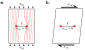
\includegraphics[scale=1]{../Figures_chap_article/crack_griffith.pdf}
\caption[Concentration des contraintes en pointe de fissure]{Représentation schématique de deux fractures. \textbf{a.}\,Fracture de longueur $\ell$ en mode d'ouverture. Une contrainte d'étirement $\sigma_{yy}$ homogène est appliquée au système. Les lignes rouges représentent les lignes de force dans le matériau. Une concentration des lignes de force indique une augmentation de la contrainte locale\,\cite{ohring_engineering_1995}. \textbf{b.}\,Fracture de longueur $\ell$ en mode de cisaillement dans le plan. Une contrainte de cisaillement $\sigma_{xy}$ homogène est appliquée au système. Les cercles rouges indiquent une concentration des contraintes.}
\label{fig:griffith_intro}
\end{figure}




Lorsqu'une contrainte $\sigma$ est appliquée aux bords d'un matériau élastique isotrope, elle est transmise à l'intérieur de celui-ci selon la loi de Hooke. Si le milieu est homogène, chaque volume infinitésimal du matériau supporte la même contrainte, mais si un défaut apparaît, il peut être le siège d'une concentration des contraintes, ce qui en fait un point de faiblesse du matériau. Une \textit{fracture}, ou \textit{crack}, ou encore \textit{rupture}, est un défaut du matériau consistant en une surface le long de laquelle les contraintes sont nulles.

Un exemple de fracture dans un matériau soumis à une contrainte d'extension est une déchirure dans une feuille mince que l'on étire (Fig.\,\ref{fig:griffith_intro}a). Lors de l'étirement de la feuille, les bords de la déchirure ne supportent aucune contrainte $\sigma_{yy}$. Sa pointe en revanche accumule de plus grandes contraintes que le reste du matériau, ce qui mène à terme à sa propagation, et à la déchirure complète de la feuille. C'est par l'existence de ce type de fractures que Griffith a répondu à la question initiale de son étude portant sur les fibres de verre. Les microfissures dans le verre, dues aux imperfections de fabrication, mènent à une accumulation de contraintes et à la rupture précoce de l'échantillon\,\cite{griffith_phenomena_1921}.












\subsubsection{Critère d'initiation de Griffith}


Si une fracture est présente dans un matériau au repos, elle ne se propage pas. Lorsque le matériau est chargé et la contrainte appliquée à l'interface est suffisante, la fracture peut s'étendre. Cette contrainte limite $\sigma_c$ dépend des propriétés du matériau, mais également de la longueur de la fracture. Afin de la déterminer il nous faut effectuer un bilan d'énergie. Deux énergies sont en jeu dans la propagation d'une fracture. La première est l'énergie potentielle élastique stockée par le matériau en raison des déformations. L'énergie potentielle élastique totale du matériau $E_{el}$ s'exprime grâce à la densité d'énergie potentielle locale $e_{el}$ par

\begin{equation}
E_{el} = \iiint e_{el}\,\mathrm{d}\mathcal{V}\qquad\text{avec}\qquad e_{el}=\frac{1}{2}\varepsilon\cdot\sigma
\end{equation}


Dans un matériau contenant une fracture, celle-ci créé une ligne de contraintes nulles, et relâche une partie de cette énergie par rapport au matériau sans défaut. L'énergie relâchée par unité de longueur du crack est notée $W$. Nous définissons $G=-\partial W/\partial\ell$ le \textit{taux de restitution d'énergie} (\textit{energy release rate}) correspondant à l'énergie libérée par la propagation de la fracture par unité de longueur. Il nous faut ensuite considérer l'énergie nécessaire à la création du défaut par unité de longueur, notée $U$. La fracture ne peut se propager que lorsque les variations de ces deux énergies linéiques avec la longueur du crack $\ell$ se compensent. Le critère de Griffith est alors que l'énergie libérée par le relâchement élastique compense l'énergie nécessaire à la création des surfaces libres, soit

\begin{equation}
\dfrac{\partial\:}{\partial\ell}\left(W-U\right)=0
\end{equation}

Dans son article fondateur Griffith considère le cas d'une plaque mince contenant une fissure de le longueur $\ell$ et soumise à une contrainte en ouverture $\sigma$ uniforme et constante, dans l'hypothèse de planéité des contraintes\,\cite{griffith_phenomena_1921}. Il montre alors que

\begin{equation}
W\propto \ell^2\sigma^2/E
\end{equation}

De plus l'énergie $U$ peut s'exprimer en fonction de la longueur de la fissure à l'aide de \textit{l'énergie de fracture} $\Gamma$, qui est une caractéristique du matériau, sous la forme

\begin{equation}
U = \Gamma \ell
\end{equation}

Ainsi le critère de Griffith devient

\begin{equation}
G=\Gamma
\end{equation}


Cette équation permet d'établir l'expression d'une contrainte limite $\sigma_c$ à partir de laquelle la fracture se propage\,\cite{griffith_phenomena_1921,freund_dynamic_1990}

\begin{equation}
\sigma_c\propto\sqrt{\frac{\Gamma E}{\ell}}
\end{equation}

Ainsi la contrainte $\sigma_c$ nécessaire pour déstabiliser une fracture est une grandeur décroissante de la longueur de celle-ci. La valeur exacte de cette contrainte dépend de la géométrie considérée. Dans le cas d'un système de taille infinie avec un chargement homogène en ouverture\,\cite{sun_fracture_2012}


\begin{equation}
\sigma_c=\sqrt{\frac{\Gamma E}{\pi\ell(1-\nu^2)}}
\end{equation}


Il est possible de considérer $\Gamma$ comme la valeur critique de $G$, notée également $G_c = \Gamma$. Conjointement la longueur de Griffith est définie comme la longueur critique $\ell_c\propto1/\sigma^{2}$ telle que $G=\Gamma$.


Ce critère nous permet de déterminer le point critique pour lequel la fracture s'initie, mais ne nous renseigne pas sur la forme que prennent les contraintes à son passage. Les contributions de G.\,R.\,Irwin et M.\,L.\,Williams (1957)\,\cite{irwin_analysis_1957,williams_stress_1957} ont éclairé ce point, et nous permettent de déterminer la forme du tenseur des contraintes au voisinage de la fracture, et en particulier à sa pointe.






\subsubsection{Facteur d'intensité des contraintes}
\begin{figure}[htb]
\centering
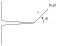
\includegraphics[scale=1]{../Figures_chap_intro/polaire.pdf}
\caption[Coordonnées polaires]{Définition des coordonnées polaires dans le cadre de la propagation d'une fracture. Le repère généralement utilisé pour décrire une fracture est solidaire de sa pointe, définissant $r$ comme la distance à celle-ci et $\theta$ l'angle par rapport à la direction de propagation.}
\label{fig:polaire}
\end{figure}


Lorsqu'un matériau contient une fissure, les tenseurs des contraintes et déformations en son sein sont altérés. En effet les coins de la fissure concentrent de fortes contraintes, tandis qu'elles sont nulles le long de la fissure. Dans le cadre de l'étude d'un solide idéalement élastique et linéaire il est possible de déterminer leur expression à proximité de la pointe de la fissure\,\cite{irwin_analysis_1957,williams_stress_1957,erdogan_fracture_2000,sun_fracture_2012}.


Nous repérons la position d'un point dans le matériau par ses coordonnées polaires $(r,\theta)$ par rapport à la pointe de la fissure (Fig.\,\ref{fig:polaire}). La résolution des équations de l'élasticité sous les hypothèses considérées donne l'expression générale du tenseur $\sigma_{ij}$ en un point $(r,\theta)$ sous la forme d'un développement en séries de Williams\,\cite{williams_stress_1957} comme suit, où les fonctions $g_{ij}^n$ sont des fonctions angulaires connues

\begin{equation}
\sigma_{ij}=\sum_{n=-1}^{+\infty} A_n\,r^{n+1/2}\,g^n_{ij}(\theta)
\end{equation}

Ce développement en puissances de $r$ ne prend que des valeurs demi-entières. Il commence en $n=-1$ pour satisfaire la convergence de l'énergie en pointe de fissure. Pour le montrer nous nous plaçons dans les coordonnées cylindriques, $\mathrm{d}\mathcal{V}(r)=r\mathrm{d\theta}\,\mathrm{d}r\,\mathrm{d}z$. Si nous considérons un des termes $\sigma = r^{\lambda}$ du développement, l'énergie élastique associée contenue en pointe de fissure dans un cercle de rayon $r$ est

\begin{equation}
\begin{aligned}
W(r)&=\frac{1}{2}\iiint\sigma\cdot\varepsilon\,\mathrm{d}\mathcal{V}(r)\propto \int_{0}^r \rho_r^{2\lambda+1}\,\mathrm{d}\rho_r
\end{aligned}
\end{equation}

Ainsi l'énergie contenue en pointe de fissure ne converge donc que si $\lambda > -1$.

À grande distance de la pointe de fissure, le tenseur des contraintes est régi par les termes tels que $n\geq0$. Cependant à proximité de la pointe, le terme en $n=-1$ diverge, et domine donc tous les autres. Par conséquent l'expression des contraintes en pointe de fissure peut être donnée par le développement limité suivant\,\cite{sun_fracture_2012}

\begin{equation}
\sigma_{ij} = \frac{K}{\sqrt{2\pi r}}f_{ij}(\theta)+\Theta\left(r^{1/2},r^{3/2},\dots\right)
\label{eq:joceline}
\end{equation}

Dans cette équation les $f_{ij}=g_{i,j}^{n=-1}$ sont des fonctions universelles dont l'expression est ·connue, et $K$ est nommé \textit{facteur d'intensité des contraintes}. Cette quantité, dont la valeur dépend de la géométrie du système et du chargement, fixe l'amplitude des contraintes subies par la pointe de fissure. Il est possible de reformuler le critère de Griffith en termes de facteur d'intensité des contraintes en définissant $K_c\sim\sqrt{\Gamma E}$ la \textit{ténacité} d'un matériau comme la valeur de $K$ lorsque $\sigma=\sigma_c$\,\cite{irwin_analysis_1957}. Cette valeur est une caractéristique du matériau. Pour le PMMA, $K_c\simeq\SI{1.1}{\mega\pascal\meter\tothe{1/2}}$\,\cite{ohring_engineering_1995}.

Le facteur d'intensité de contraintes $K$ prend la forme du produit de la contrainte à grande distance du crack et d'un facteur géométrique dépendant de la longueur du crack, il est donc possible de le calculer pour des géométries simples. Dans le cas général le calcul peut se décomposer par linéarité en un jeu de trois équations indépendantes selon des modes, comme présenté dans la section suivante.

Lorsque la contrainte atteint la limite de plasticité du matériau $\sigma_Y$ (Fig.\,\ref{fig:yield}), les déformations ne peuvent plus être considérées comme élastiques. La zone dans laquelle l'expression obtenue avec l'hypothèse d'élasticité n'est plus valable est nommée \textit{zone de régularisation des contraintes} (\textit{process zone}). Les considérations énergétiques associées aux phénomènes non-linéaires ayant lieu dans cette zone sont incorporées dans une définition plus générale de l'énergie de fracture.



\subsubsection{Modes de fracture}


\begin{figure}[htb]
\centering
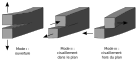
\includegraphics[scale=1]{../Figures_chap_intro/modes.pdf}
\caption[Modes de fracture]{Représentation des trois modes de fracture. Chaque mode évolue indépendamment des deux autres, ce qui permet de décomposer la solution générale des équations de la mécanique de la fracture linéaire élastique sur chacun d'eux.}
\label{fig:modes}
\end{figure}


Les fractures peuvent être décomposées en 3 modes selon le mode de chargement, c'est à dire la direction des contraintes appliquées relativement à leur direction de propagation\,\cite{freund_dynamic_1990,sun_fracture_2012} (Fig.\,\ref{fig:modes}). La fracture en ouverture est dite de \textit{mode\:\textsc{i}}, la contrainte nulle le long de la fracture est $\sigma_{yy}$. La contrainte nulle le long d'une fracture en cisaillement dans le plan, dite de \textit{mode\:\textsc{ii}}, est la contrainte cisaillante $\sigma_{xy}$. Le mode\:\textsc{iii} pour sa part correspond à un cisaillement hors du plan de propagation de la fracture. Il se caractérise par le fait que seuls les $\sigma_{zj}$ ne sont pas nuls partout. Dans le cadre de la fracture linéaire, en raison de la linéarité, ces trois modes peuvent être étudiés indépendamment, leurs contributions sont alors superposées pour décrire une fracture en mode mixte.

\newpage

Ainsi il est possible de décomposer $[\sigma]$ selon chacun de ces modes

\begin{equation}
[\sigma]=\sum_{\textsc{m}=\textsc{i,ii,iii}}[\sigma^\textsc{m}]
\end{equation}


Nous pouvons ensuite définir un facteur d'intensité des contraintes $K_\textsc{m}$ pour chaque mode puis décomposer l'Équation\,\ref{eq:joceline} comme

\begin{equation}
\sigma_{ij} = 
\sum_{\textsc{m}\in\{\textsc{i,ii,iii}\}}
\sigma_{ij}^\textsc{m}
\quad\text{avec}\quad
\sigma_{ij}^\textsc{m}=
\frac{K_\textsc{m}}{\sqrt{2\pi r}}f_{ij}^\textsc{m}(\theta)+\Theta\left(r^{1/2},r^{3/2},\dots\right)
\label{eq:sigmamodes}
\end{equation}




Les expressions des fonctions $f_{ij}^\textsc{m}$ sont alors les suivantes\,\cite{sun_fracture_2012}



\begin{equation}
\resizebox{150mm}{!}{
$
\begin{cases}
	f^\textsc{i}_{xx}&=\left(1-\sin\frac{\theta}{2}\,\sin\frac{3\theta}{2} \right)\cos\frac{\theta}{2}\\[.5em]
	f^\textsc{i}_{yy}&=\left(1+\sin\frac{\theta}{2}\,\sin\frac{3\theta}{2} \right)\cos\frac{\theta}{2}\\[.5em]
	f^\textsc{i}_{xy}&=\sin\frac{\theta}{2}\,\cos\frac{3\theta}{2}\,\cos\frac{\theta}{2}
\end{cases}
\quad
\begin{cases}
	f^\textsc{ii}_{xx}&=-\left(2+\cos\frac{\theta}{2}\,\cos\frac{3\theta}{2}\right)\sin\frac{\theta}{2}\\[.5em]
	f^\textsc{ii}_{yy}&=\cos\frac{\theta}{2}\,\cos\frac{3\theta}{2}\,\sin\frac{\theta}{2}\\[.5em]
	f^\textsc{ii}_{xy}&=\left(1-\sin\frac{\theta}{2}\,\sin\frac{3\theta}{2} \right)\cos\frac{\theta}{2}
\end{cases}
\quad
\begin{cases}
	f^\textsc{iii}_{zx}&=-\sin\frac{\theta}{2}\\[.5em]
	f^\textsc{iii}_{zy}&=\cos\frac{\theta}{2}\\
\end{cases}
$}
\end{equation}

L'expression de $f_{zz}^{\textsc{i},\textsc{ii}}$ dépend de l'hypothèse de planéité choisie
\begin{equation}
f_{zz}^{\textsc{i},\textsc{ii}}=
\begin{cases}
0&\quad\text{planéité des contraintes}\\
\nu(f_{xx}+f_{yy})&\quad\text{planéité des déformations}
\end{cases}
\end{equation}


L'expression des fonctions $f^\textsc{m}_{ij}$ en $\theta=0$ permet de donner une expression des $K_\textsc{m}$ permettant notamment leur mesure :

\begin{equation}
\begin{aligned}
K_\textsc{i}&=\lim_{\:r\rightarrow 0^+}\sqrt{2\pi r}\;\sigma_{yy}(r,\theta=0)\\
K_\textsc{ii}&=\lim_{\:r\rightarrow 0^+}\sqrt{2\pi r}\;\sigma_{xy}(r,\theta=0)\\
K_\textsc{iii}&=\lim_{\:r\rightarrow 0^+}\sqrt{2\pi r}\;\sigma_{zy}(r,\theta=0)
\end{aligned}
\end{equation}


La séparation de l'Équation\,\ref{eq:joceline} en modes indépendants permet également de définir des valeurs de $G$ par mode, notées $G_\textsc{m}$. L'expression complète de $G$ est alors donnée par
\begin{equation}
G=\frac{1-\nu^2}{E}\left(K_\textsc{i}^2+K_\textsc{ii}^2\right) + \frac{1+\nu}{E}K_\textsc{iii}^2
\end{equation}






\begin{figure}[p]
\centering
\begin{tabular}{lccc}
Matériau & $\Gamma\left(\mathrm{kJ.m}^{-2}\right)$ & $K_{I c}\left(\unit{\mega\pascal\meter\tothe{1/2}}\right)$ & $E(\mathrm{GPa})$ \\
\hline & & & \\
Acier allié & 107 & 150 & 210 \\
Aluminium allié & 20 & 37 & 69 \\
Acier & 12 & 50 & 210 \\
Caoutchouc & 13 & - & 0.001 \\
époxy & 2 & 2.2 & 2.4 \\
PMMA & 0.5 & 1.1 & 2.5 \\
Polystyrène & 0.4 & 1.1 & 3 \\
Bois & 0.12 & 0.5 & 2.1 \\
Verre & 0.007 & 0.7 & 70 \\
\hline
\end{tabular}
\caption[Caractéristiques de différents matériaux]{Caractéristiques de différents matériaux pour une fracture en mode\:\textsc{i} (extrait de\,\cite{ohring_engineering_1995}). Il est possible de montrer que $\Gamma\simeq K^2/E$.}
\label{tab:caracmater}
\end{figure}


\begin{figure}[p]
\centering
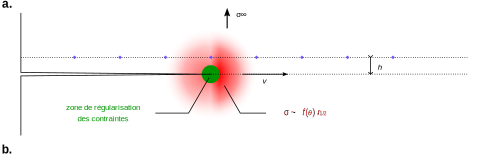
\includegraphics[scale=1]{../Figures_chap_intro/LEFM_plot_mesure.pdf}
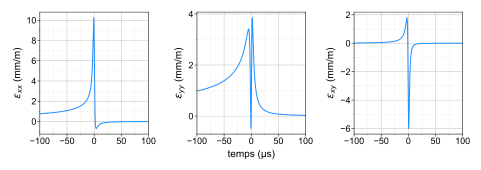
\includegraphics[scale=1]{../Figures_chap_intro/LEFM_plot.pdf}
\caption[Simulation d'une rupture dynamique en mode \textsc{i}]{\textbf{a.}\,Propagation et mesure d'une rupture en mode\:\textsc{i}. La rupture se propage le long de la ligne pointillée du bas à une vitesse $v$. Les capteurs de déformation mesurant $\varepsilon$ sont disposés le long de la ligne pointillée du haut, à une distance $h$ de la ligne de propagation de la rupture. Afin de mesurer le passage de la rupture et sa forme caractéristique, la distance $h$ doit être choisie supérieure au rayon de la zone de régularisation mais dans la zone où le terme en $\sigma\sim r^{-1/2}$ domine le développement en série de Williams. \textbf{b.}\,Évolution de $\varepsilon$ en fonction du temps au passage d'une fracture à $h=\SI{1}{\milli\meter}$ du point de mesure. L'oscillation en vaguelette observée est la signature de la fonction angulaire $\Sigma_{ij}^\textsc{m}$. La fracture se déplace à $v=\SI{500}{\meter\per\second}$, et l'énergie de fracture du matériau est $G=\SI{2}{\kilo\joule\per\meter\squared}$ (similaire à du PMMA).}
\label{fig:simulfrac}
\end{figure}








En résumé, nous avons vu qu'au sein d'un matériau, la pointe d'une rupture statique ou quasi-statique de longueur $\ell$ est le siège d'une concentration des contraintes. Le critère d'initiation de rupture de Griffith indique que lorsque le taux de restitution d'énergie $G$ est égal à l'énergie de fracture du matériau $\Gamma$ (Fig.\,\ref{tab:caracmater}), la fracture peut se propager, permettant la définition d'une contrainte limite $\sigma_c$ pour une rupture de longueur $\ell$. Cette contrainte s'exprime comme $\sigma_c\propto\sqrt{\Gamma E/\ell}$, le facteur de proportionnalité dépendant de la géométrie considérée. La contrainte en pointe de fissure s'exprime comme une série de Williams dont le terme dominant à proximité de la pointe de fissure est $\sigma\propto K/\sqrt{r}$, avec $K$ le facteur d'intensité des contraintes, qui lorsque la contrainte atteint $\sigma_c$ vaut $K = K_c$ la ténacité du matériau (Fig.\,\ref{tab:caracmater}). Nous avons enfin vu qu'il était possible de décrire tout crack comme la superposition de trois modes indépendants par linéarité. Cette séparation permet notamment de redéfinir les caractéristiques du matériau et critère d'initiation par mode.

Les trois modes ont leur propre critère d'initiation, et leur équation de propagation. L'évolution de la rupture est alors décrite par les lois de la fracture dynamique.


\subsection{Fracture dynamique}





Une fois déstabilisée, une rupture peut se propager dynamiquement dans le matériau. Si sa vitesse $v$ est telle que $v<c_r$ la vitesse des ondes de Rayleigh dans le matériau, la rupture est dite \textit{sub-Rayleigh}. Elle est alors décrite par la mécanique de la fracture linéaire élastique. Si cependant elle se déplace à $v>c_s$ la vitesse des ondes de cisaillement, elle est dite \textit{supershear}. Dans ce cas, la convergence du flux d'énergie élastique en point de fissure ne permet pas d'expliquer sa propagation, qui dépend d'un cadre physique différent\,\cite{dunham_supershear_2003}.

\subsubsection{Expression du tenseur des contraintes}


Dans le cas des ruptures sub-Rayleigh sous un chargement constant, l'expression de $\sigma_{ij}^\textsc{m}$ dépend de la vitesse, et en particulier des rapports $\alpha_s =\sqrt{ 1-(v/c_s)^2}$ et $\alpha_p =\sqrt{ 1-(v/c_p)^2}$ où $c_p$ et $c_s$ sont les vitesses des ondes de compression et de cisaillement dans le matériau. L'expression des facteurs d'intensité des contraintes est alors donnée par

\begin{equation}
K_\textsc{m}(v)=K_\textsc{m}^S\times k_\textsc{m}^d(v)
\end{equation}

Dans cette expression $K_\textsc{m}^S = K_\textsc{m}(v=0)$ correspond au facteur d'intensité des contraintes statique ou quasi-statique, et $k_\textsc{m}^d(v)$ est une fonction connue de la vitesse de propagation. Cette expression n'est valide que pour un système quasi-infini, pour lequel les ondes émises par la rupture n'ont pas eu le temps de se réfléchir sur un bord. Sous cette hypothèse il est possible de calculer $K_\textsc{m}(v)$.

Les fonction $f_{ij}^\textsc{m}(\theta)$ dans l'Équation\,\ref{eq:sigmamodes} sont également remplacées par des fonctions dynamiques $\Sigma_{ij}^\textsc{m}(\theta,v)$ connues, exhibant en modes \textsc{i} et \textsc{ii} une divergence lorsque $v\rightarrow c_r$, et lorsque $v\rightarrow c_s$ en mode \textsc{iii}. L'expression du tenseur des contraintes en pointe de fissure est alors donnée par\,\cite{sun_fracture_2012}


\begin{equation}
\sigma_{ij}^\textsc{m}=\frac{K_\textsc{m}^Sk^d_\textsc{m}(v)}{\sqrt{2\pi r}}\Sigma^\textsc{m}_{ij}(\theta,v)+\Theta(r^{1/2},r^{3/2},\dots)
\label{eq:sigmamodedyn}
\end{equation}

Lors du passage d'une rupture à proximité d'un capteur de déformation, la coordonnée $\theta$ repérant le point de mesure dans le référentiel de la pointe de fissure passe de $\theta\rightarrow\SI{0}{\degree}$ à $\theta\rightarrow\SI{180}{\degree}$. Ainsi la mesure balaie la fonction angulaire $\Sigma_{ij}^\textsc{m}$ et exhibe une variation caractéristique en vaguelette (Fig.\,\ref{fig:simulfrac}). La mesure de $\varepsilon$ au passage de la rupture permet de déterminer $\Gamma$ par un ajustement\,\cite{svetlizky_brittle_2019}.

\newpage


\subsubsection{Critère de propagation}

Le critère de propagation d'une rupture dynamique est identique au critère d'initiation d'une rupture statique, c'est à dire que le taux de restitution d'énergie $G$ doit être égal à l'énergie de fracture $\Gamma$, mais $G$ dépend de la vitesse de propagation. Il est possible d'exprimer $G$ sous la forme

\begin{equation}
G(v)\propto\frac{K^2}{E}\times A(v)\quad\text{et}\quad G(v) = \Gamma
\label{eq:propagfracdyn}
\end{equation}

La fonction $A(v)$, nommée facteur dynamique, prend en mode\:\textsc{i} et \textsc{ii} la forme

\begin{equation}
A(v)=\dfrac{\alpha_p(1-\alpha_s^2)}{4\alpha_p\alpha_s-(1+\alpha_p^2)^2}
\end{equation}

Ce facteur diverge lorsque $v\rightarrow c_r$ la vitesse des ondes de Rayleigh, correspondant à la première racine réelle du dénominateur de $A(v)$. Cette égalité indique que l'énergie nécessaire à la propagation d'une rupture sub-Rayleigh en mode\:\textsc{i} ou \textsc{ii} diverge lorsque la vitesse de propagation approche $c_r$, ce qui en fait la vitesse maximale de ce type de rupture. Pour une rupture en mode\:\textsc{iii} la vitesse limite est $c_s$.






\subsection{Fracture frictionnelle}
\label{sec:LEFMfric}



Pour décrire la mise en glissement d'une interface frictionnelle,
l'extension spatiale de celle-ci doit être considérée, contrairement à l'approche adoptée dans les modèles Rate-and-State, qui décrivent le mouvement du centre de masse du système
(Sec.\,\ref{sec:rateandstate}). En effet cette initiation du mouvement est due à un affaiblissement de l'interface par un front propagatif qui peut s'assimiler à un front de rupture. Il a été montré que ce front est une fracture en mode de cisaillement décrite par la mécanique de la fracture linéaire élastique\,\cite{svetlizky_brittle_2019}. Dans cette section nous présentons les spécificités théoriques de la fracture frictionnelle.


\subsubsection{Phénoménologie}

Une rupture fragile classique amorcée en un point de l'espace se propage dans le matériau alentour en raison de l'accumulation des contraintes en sa pointe, rompant le bloc le long de sa trajectoire. Dans le cas d'une rupture frictionnelle, l'interface est pressée et chargée à grande distance et accumule des contraintes cisaillantes. La rupture peut alors nucléer en un point de l'interface où un microcontact atteint sa résistance au cisaillement, se rompt et se met en glissement (Sec.\,\ref{sec:microfric}). Cette mise en glissement reporte les contraintes que le contact portait sur les aspérités avoisinantes, rompant de proche en proche ces microcontacts le long de l'interface. La rupture peut se propager ainsi tout le long de l'interface, jusqu'à avoir affaibli tous les contacts, permettant le glissement inertiel des blocs. Ces ruptures, comme les ruptures en mode de cisaillement classique, se propagent à des vitesses $v$ telles que $v<c_r$ la vitesse des ondes de Rayleigh dans le matériau, ou telles que $v>c_s$ la vitesse des ondes de cisaillement.

Le mouvement de glissement macroscopique des deux blocs est un mouvement inertiel, il ne commence qu'après que la rupture a traversé l'interface entière. Lorsque les blocs ont relâché une quantité suffisante des contraintes cisaillantes, le glissement s'arrête et les microcontacts se reforment (Sec.\,\ref{sec:evolutionmacro}). L'interface peut alors se recharger, et entrer par exemple dans un cycle de stick-slip, pour lequel chaque évènement de slip est initié par une rupture.

Nous présentons dans la section suivante que la propagation de ces ruptures est régie par la mécanique de la fracture.


\subsubsection{Description par la mécanique de la fracture}

La fracture frictionnelle est une fracture en mode\:\textsc{ii}, guidée par un plan faible formé par l'interface. Ce guidage est une composante essentielle de sa propagation, car dans un solide intact, une fracture initiée en mode\:\textsc{ii} est instable, et évolue spontanément vers le mode\:\textsc{i}. Le long de l'interface frictionnelle, l'énergie de fracture associée à l'affaiblissement des microcontacts $\Gamma_\textsc{fric}$ est beaucoup plus faible que celle associée à une fracture du matériau intact $\Gamma_\textsc{bulk}$. Guidée par l'interface, la rupture peut être repérée par la coordonnée $x(t)$ de son front, et il n'est pas exclu que $\Gamma_\textsc{fric}$ dépende de $x$. Ainsi à partir de l'Équation\,\ref{eq:propagfracdyn} nous pouvons écrire

\begin{equation}
\Gamma_\textsc{bulk} \gg \Gamma_\textsc{fric}
\quad\text{et}\quad
G_\textsc{ii}(v) = \Gamma_\textsc{fric}(x)
\end{equation}


Une différence majeure entre une fracture classique et une rupture frictionnelle est que la rupture frictionnelle n'est pas une ligne de contraintes nulles. En effet, là où après le passage d'une rupture classique le matériau est endommagé de manière irréversible, la rupture frictionnelle affaiblit des microcontacts et leur permet de se mettre en mouvement. Les microcontacts supportent toujours après le passage de la rupture une contrainte cisaillante résiduelle $\sigma_{xy} =\sigma_r$ (Sec.\,\ref{sec:microfric}). De plus pour une rupture en mode de cisaillement les contraintes initiales le long de la ligne de propagation de la rupture sont

\begin{equation}
\big[\sigma^\textsc{ii}\big] (\theta = 0,\,r\rightarrow+\infty) = \begin{bmatrix}
0 & \sigma_{xy}^0\\
\sigma_{xy}^0 & 0
\end{bmatrix}
\label{eq:initnormal}
\end{equation}

Ainsi afin de ramener le tenseur des contraintes $[\sigma^\textsc{fric}]$ d'une rupture frictionnelle à celui d'une fracture en mode de cisaillement, la linéarité des équations présentées permet de prendre en compte les conditions initiales par superposition

\begin{equation}
\big[\sigma^\textsc{ii}\big] = 
\big[\sigma^\textsc{fric}\big] -
\begin{bmatrix}
\sigma_{xx}^0 & \sigma_r\\
\sigma_r      & \sigma_{yy}^0
\end{bmatrix}
\label{eq:pmpi}
\end{equation}


Il a de plus été montré que les contraintes divergent en pointe de fissure selon les équations de la mécanique de la fracture linéaire élastique\,\cite{svetlizky_classical_2014}. Elle est dont décrite par l'Équation\,\ref{eq:sigmamodedyn} avec $\textsc{m}=\textsc{ii}$ seulement, c'est à dire





\begin{equation}
\sigma_{ij}^\textsc{fric}
=
\frac
	{K_{\textsc{ii}}(v)}
	{\sqrt{2\pi r}}
\times
	\Sigma_{ij}^{\textsc{ii}}
(\theta,v)
+
\begin{bmatrix}
	\sigma_{xx}^0 & \sigma_r\\
	\sigma_r      & \sigma_{yy}^0
\end{bmatrix}
\label{eq:fracdynfric}
\end{equation}

Dans cette équation $K_\textsc{ii}$ est le facteur d'intensité des contraintes lié à l'énergie de fracture de l'interface frictionnelle $\Gamma = \Gamma_\textsc{fric}$. Cette énergie correspond à l'énergie nécessaire pour affaiblir les microcontacts à l'interface, elle est donc directement liée à l'aire réelle de contact $A_r$, elle-même proportionnelle à $\sigma_{yy}$\,\cite{svetlizky_brittle_2019}. Ainsi

\begin{equation}
\Gamma(x)\propto\sigma_{yy}(x)
\label{eq:homospa}
\end{equation}

Cette rupture frictionnelle a été largement étudiée dans le cas des interfaces solide-solide homogènes, comme présenté dans le Chapitre\:\ref{chap:etatdelart}.

Nous avons au cours de cette section montré que le mouvement de glissement rapide d'une interface frictionnelle est initié par la propagation d'une fracture le long de l'interface. Cette fracture est décrite de manière quantitative par la mécanique de la fracture linéaire élastique. Une question est de savoir si cette description est généralisable à des interfaces complexes comme celles étudiées en mécanique des failles, bien que leur comportement en découle. L'étude de celles-ci est présentée dans la section suivante.

\newpage








\section{Mécanique des failles}
\label{sec:failles}






La mécanique des failles est le domaine de la géophysique étudiant les mécanismes de déformations des roches et des failles sismiques, au travers d'échelles de temps et d'espace très diverses. Dans le cadre de notre étude d'une faille en laboratoire nous cherchons à caractériser des mouvements de glissement rapide à l'interface, qui s'apparentent à des séismes, un des objets d'étude de la mécanique des failles. Nous présentons dans cette section les principes de base de l'étude des mouvements lithosphériques, de la tectonique des plaques, et de la mesure et la caractérisation des séismes.


\begin{figure}[hbt]
\centering
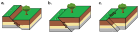
\includegraphics[scale=1]{../Figures_chap_article/failles.pdf}
\caption[Types de failles]{Les trois grands types de failles. La faille normale (\textbf{a}) apparaît dans les systèmes en extension. La faille inverse (\textbf{b}) apparaît dans les systèmes en compression comme les zones de subduction. La faille transformante (\textbf{c}) apparaît dans les zones de coulissement entre des plaques tectoniques.}
\label{fig:typesdefailles2}
\end{figure}

\subsection{Qu'est-ce qu'une faille ?}

En géologie, une \textit{faille} est un plan ou une zone de rupture entre deux blocs rocheux qui sont en déplacement relatif. Les failles peuvent être de grandes dimensions, comme les failles tectoniques, ou millimétriques. Ces failles peuvent former des plans de ruptures très nets et très actifs, comme la faille de San Andreas à l'ouest des États-Unis\,\cite{scholz_evidence_2000}, ou de grandes zones de rupture contenant de multiples failles individuellement peu actives comme le rift est-africain\,\cite{chorowicz_east_2005}.




\subsubsection{Origine des failles}


La croûte terrestre, ou \textit{lithosphère}, est composée de plaques en mouvement relatif. Ces plaques, dites \textit{plaques tectoniques}, d'une épaisseur d'environ \SI{100}{\kilo\meter}\,\cite{pollack_regional_1977}, sont composées de roches basaltiques et granitiques solides et rigides, et reposent sur l'\textit{asthénosphère}, ou manteau terrestre, composé pour sa part de péridotites dans un état solide, mais ductile (Fig.\,\ref{fig:tecto}a). Le manteau, d'une épaisseur de l'ordre de \SI{3000}{\kilo\meter}, a une viscosité de l'ordre de $10^{18}$ à $10^{22}$\,Pa.s  contre $10^{25}$ pour la lithosphère\,\cite{cathles_viscosity_2015}, et peut ainsi, sous l'influence des gradients de température au sein de la Terre, adopter un mouvement de convection (Fig.\,\ref{fig:tecto}b). Ces mouvements forment des rouleaux, qui entraînent avec eux les plaques tectoniques à des vitesses allant jusqu'à \SI{10}{\centi\meter} par an.

De nombreux phénomènes géologiques ont lieu à l'interface entre les plaques tectoniques. Les zones d’accrétion, situées à l'interface entre deux plaques en éloignement, sont le siège d'un volcanisme à l'origine par exemple de la dorsale Atlantique qui émerge en Islande. Dans les zones de collision entre deux plaques, les mouvements tectoniques sont responsables de la subduction de la lithosphère océanique, engendrant du volcanisme d'arc, partiellement à l'origine de la lithosphère continentale\,\cite{stern_subduction_2002,Hawkesworth_generation_2010}. Des mouvements de coulissement entre les plaques tectoniques peuvent également se produire, comme c'est le cas le long de la faille de San Andreas\,\cite{anderson_san_1971, okubo_fractal_1987,zoback_new_1987, powell_evolution_1992, linde_slow_1996, tan_connecting_2020}. Les failles ont une morphologie sculptée par le temps et les contraintes qu'elles subissent.

\begin{figure}[hbt]
\centering
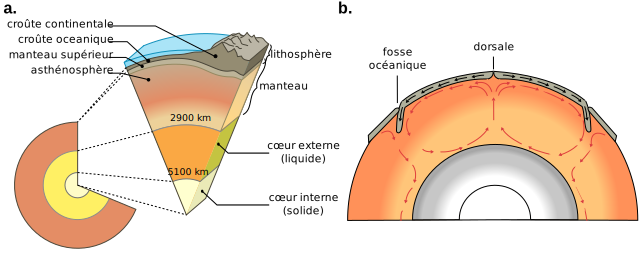
\includegraphics[scale=1]{../Figures_chap_intro/coupeterre.pdf}
\caption[Structure interne de la Terre]{Schéma de la structure interne de la Terre et du mécanisme par lequel les mouvements de convection du manteau sont à l'origine de la tectonique des plaques.}
\label{fig:tecto}
\end{figure}


\subsubsection{Anatomie d'une faille}



Une faille est un système géophysique complexe, centré sur un plan de faille, et composé de multiples couches de roches structurellement et chimiquement différentes. Lorsque deux blocs de roches en contact sont soumis à un déplacement relatif, ils subissent des contraintes et déformations menant à la fragilisation et à l'usure des roches. Il est ainsi possible d'observer de part et d'autre du plan de faille une succession de couches géologiques aux propriétés variées.

À grande distance du plan de faille, la roche mère forme un bloc solide, accumulant de l'énergie élastique au travers des déformations qu'elle subit. En s'approchant de la faille et en entrant dans la zone d'endommagement, celle-ci devient une \textit{cataclastite}, une roche de faille fracturée, broyée et stratifiée par le déplacement relatif des deux blocs en contact (Fig.\,\ref{fig:faillereelle}). Au centre de la zone de faille se trouve la zone cœur, composée de brèche de faille et de gouge, une roche granulaire non cohésive\,\cite{woodcock_classification_2008}. Au delà des différences de granulométrie, la différence de porosité entre ces couches introduit également des différences chimiques et métamorphiques. Enfin les failles sismiques ont une extension spatiale en profondeur, des séismes pouvant se produire jusqu'à 600 kilomètres sous la surface\,\cite{frohlich_nature_1989}. Chaque système de faille a sa morphologie propre.


\begin{figure}[h!]
\centering
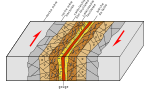
\includegraphics[scale=1]{../Figures_chap_article/realfault.pdf}
\caption[Anatomie d'une faille]{Anatomie schématique d'une faille sismique réelle. La faille est composée de multiples couches de roches, plus ou moins cohésives et fracturées. Les couches de brèche et de gouge sont des milieux granulaires au cœur de la faille (adapté de\,\cite{treffeisen_fault_2021}).}
\label{fig:faillereelle}
\end{figure}



\subsection{Étude des séismes}


Lorsque deux plaques tectoniques sont en contact, elles sont soumises à des forces de frottement solide. Les zones la plupart du temps bloquées en surface sont toujours soumises aux contraintes appliquées par les déplacements de l'asthénosphère, et accumulent de l'énergie élastique au travers de leurs déformations. Lorsqu'elles se débloquent, un évènement de glissement rapide a lieu. Cet évènement, relâchant l'énergie élastique accumulée, dure généralement au plus quelques secondes, et émet des ondes de déformations qui se propagent dans les roches alentour, parfois jusqu'à la surface. C'est ce mécanisme que l'on nomme \textit{séisme}.

%Les roches en contacts sont plus ou moins visqueuses selon les conditions de température et de pression dans lesquelles elles évoluent\,\cite{mccaffrey_slow_2008}, 



\subsubsection{Le stick-slip comme description du cycle sismique}

Les séismes sont la manifestation d'un mouvement de stick-slip. Cette observation, publiée en 1966 par W.\,F.\,Brace et J.\,D.\,Byerlee\,\cite{brace_stick-slip_1966}, s'appuyant alors sur les études menées en laboratoire sur des roches naturelles\,\cite{jaeger_frictional_1959,uffen_stress_1963,griggs_observations_1960}, est un fondement de l'étude moderne de la sismicité, remplaçant la théorie du rebond élastique de Reid\,\cite{reid_mechanics_1910}. Le mouvement de stick-slip est en effet caractéristique des dynamiques régies par les frottements solides (Sec.\,\ref{sec:ss1}).

Dans les mouvements géologiques ce mouvement de stick-slip ne se caractérise cependant pas par sa régularité, puisqu'il est très difficile de prédire les séismes\,\cite{rikitake_earthquake_1968, mogi_earthquake_1985, geller_earthquake_1997, kanamori_earthquake_2003}. La prédiction et prévention de ceux-ci est pourtant un enjeu majeur, et la compréhension des mécanismes microscopiques sous-jacents au frottement solide en est une clé. L'étude de ces mécanismes a mené à de nombreux modèles empiriques (Sec.\,\ref{sec:rateandstate}) appuyés par des observations de terrain permettant de décrire le comportement des failles et de rendre compte de ce phénomène de stick-slip à l'échelle des temps géologique.


\subsubsection{Magnitude et moment sismique}

Un séisme est la manifestation d'un glissement le long d'une interface frictionnelle. Il s'accompagne d'une dissipation d'énergie (Éq.\,\ref{eq:dissip}) et de l'émission et la propagation d'ondes dans les roches. La mesure de ces phénomènes permet de définir des grandeurs utiles à la caractérisation, au catalogage et à l'étude statistique des séismes. Nous définissons ici plusieurs de ces observables.


\myparagraph{Le déplacement moyen}

\begin{figure}[htb]
\centering
\includegraphics[width=.8\textwidth]{../Figures_chap_intro/fence.jpg}
\caption[Observation directe du glissement dû à un séisme]{Photographie des effets du tremblement de terre de 1906 à San Francisco, causé par la rupture d'une portion de la faille de San Andreas. La faille a glissé d'environ \SI{2.5}{\meter} le long d'un plan de fissure particulièrement bien défini\,\cite{reid_mechanics_1910}.}
\label{fig:fence}
\end{figure}

Le déplacement moyen est la moyenne de la distance glissée le long de la faille ou portion de faille rompue lors d'un séisme (Fig.\,\ref{fig:fence}). Son évaluation peut être effectuée par mesure directe des glissements sur le terrain, cependant dès lors que le mouvement est faible, ou que la zone de faille est étendue, elle perd en précision. Des techniques d'imagerie satellite ou de mesure par balises GPS permettent de raffiner ces mesures à une précision de l'ordre du centimètre, et de déterminer le champ des déformations dans toute la lithosphère\,\cite{michel_measuring_1999,segall_gps_1997,pagani_quantification_2021}. La mesure des déplacements en surface ne suffit cependant pas à caractériser un séisme, puisque certains mouvements profonds ne s'accompagnent pas d'un glissement en surface. Pour les caractériser des grandeurs liées à l'énergie qu'ils relâchent sont utilisées.


\myparagraph{Les magnitudes}

La \textit{magnitude} d'un séisme est une grandeur sans unité évaluant l'énergie libérée par ce séisme sur une échelle logarithmique. Sa définition a évolué au cours du temps, en fonction de la grandeur mécanique utilisée pour la mesurer. Historiquement la première définition est celle de Richter en 1935 de la magnitude locale $M_L$\,\cite{richter_instrumental_1935}. Elle est basée sur les mesures des ondes sismiques par des sismographes, appareils combinant des accéléromètres et vélocimètres, et est définie comme

\begin{equation}
M_L=\log(D)-\log(D_0)+c\times\log(\Delta)
\end{equation}

Dans cette équation, $D$ désigne l'amplitude maximale mesurée sur le sismogramme utilisé pour la mesure, $\Delta$ la distance à l'épicentre, $c$ une constante d'étalonnage, et $D_0$ une amplitude de référence déterminant ce que l'on considère comme la valeur de $D$ pour un séisme de magnitude $M_L=0$ perçu à \SI{100}{\kilo\meter}. Cette définition est aujourd'hui limitée à des études locales, car elle dépend de paramètres empiriques locaux, étalonnés par zone de faille. Cette limitation à mené à la définition des \textit{magnitudes d'ondes} basées chacune sur la mesure d'un type d'onde spécifique. Les deux magnitudes d'ondes sont celle des ondes de surface $M_S$ et celle des ondes de volume (\textit{body waves}) $m_b$ toutes deux introduites par Gutenberg et Richter en 1936 et 1956\,\cite{gutenberg_magnitude_1936,gutenberg_earthquake_1956}. Toujours en usage aujourd'hui, elles demeurent empiriques et basées sur des étalonnages, et subissent un phénomène de saturation lorsque $M_S$ ou $m_b>9$\,\cite{kanamori_energy_1977, howell_saturation_1981}.

La magnitude la plus couramment utilisée aujourd'hui est la \textit{magnitude de moment} $M_w$ introduite par Hanks et Kanamori en 1979\,\cite{hanks_moment_1979}, liée directement à l'énergie libérée par le séisme et au moment sismique. Elle est particulièrement utilisée pour les séismes de grande magnitude ($M>4$), tandis que les magnitudes d'ondes sont privilégiées pour les faibles magnitudes.

\myparagraph{Le moment sismique}

le \textit{moment sismique} $M_0$ est une mesure de l'énergie libérée par un séisme par l'évaluation du travail des forces responsables du glissement. À longue distance un séisme peut en effet être vu comme le résultat de l'application d'un double couple de forces\,\cite{kagan_3-D_1991} résultant en une déformation élastique des roches. Le moment s'exprime alors comme

\begin{equation}
M_0=\frac{E}{2(1+\nu)}\times A\times d
\end{equation}

Dans cette équation $G_s=E/2(1+\nu)$ est le module de cisaillement, $A$ est la surface macroscopique du plan de fracture rompue durant l'évènement, et $d$ est le déplacement moyen à l'interface. La magnitude de moment est alors définie comme

\begin{equation}
M_w=\frac{2}{3}\log_{10}(M_0)-6.07
\label{eq:magnitude}
\end{equation}

Une augmentation d'un point de magnitude correspond à une multiplication par 30 du moment sismique. La magnitude est ainsi définie sur une échelle à valeurs dans $\mathbb{R}$ nommée \textit{échelle de Richter}\,\cite{kanamori_quantification_1978}. L'échelle est théoriquement illimitée, cependant le séisme le plus fort enregistré est le séisme de 1960 à Valdivia au Chili, avec une magnitude $M_w=9.5$\,\cite{ruiz_historical_2018}. Les tremblements de terre d'une telle magnitude n'ont lieu qu'une à trois fois par siècle, et relâchent une quantité suffisante d'énergie pour altérer l'axe de rotation de la Terre et changer la longueur du jour de quelques microsecondes\,\cite{chao_changes_1987}. Bien que l'échelle n'ait théoriquement pas non plus de minimum, les séismes de magnitude inférieure à 1 sont très difficilement détectables et se produisent en continu sur Terre. Ils peuvent même être dus aux activités humaines, un séisme de magnitude 0 relâchant une quantité d'énergie équivalente à celle libérée par la
chute d'un objet d'une tonne d'une hauteur de \SI{5}{\meter}.
%\href{https://youtu.be/e3uk7jU3RHo}{\textcolor{black}{chute d'un objet d'une tonne d'une hauteur de \SI{5}{\meter}}.}

Dans le but de décrire et prévenir les risques sismiques, le moment sismique et la magnitude font l'objet d'études statistiques et de modèle empiriques, comme la loi de Gutenberg-Richter.


\subsubsection{Loi de Gutenberg Richter}

\label{sec:gutricht}

\begin{figure}[htb]
\centering
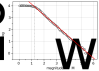
\includegraphics[scale=1]{../Figures_chap_intro/grlaw.pdf}
\caption[Loi de Gutenberg-Richter]{Distribution fréquence-magnitude cumulée des évènements sismiques dans la région de Abruzzi en Italie, entre avril 2007 et avril 2010 (adapté de\,\cite{de_santis_gutenberg-richter_2011}). Un séisme de magnitude $M_w=6.3$ a eu lieu dans la zone surveillée le 6 avril 2009. Un ajustement de la portion linéaire de la distribution (ligne rouge) permet une estimation globale des paramètres de la loi de Gutenberg-Richter ($b=0.89\pm0.03$). La ligne verticale en pointillés représente une estimation de la magnitude minimale à partir de laquelle les sismographes perdent leur sensibilité.}
\label{fig:grlaw}
\end{figure}

La loi de Gutenberg-Richter est une loi empirique décrivant la distribution de magnitude des séismes dans un réseau de failles donné\,\cite{gutenberg_frequency_1944}. Cette loi exprime un lien entre la magnitude $M$ et le nombre total de séismes d'une magnitude inférieure à $M$ ou \textit{distribution fréquence-magnitude cumulée} noté $N_{>M}$. La loi de Gutenberg-Richter prédit qu'il existe des constantes $a$ et $b$ telles que
\begin{equation}
\log_{10}N_{>M}=a-bM
\label{eq:grlaw}
\end{equation}


La loi de Gutenberg-Richter, bien qu'empirique, dispose d'un bon accord avec les données des relevés sismiques (Fig.\,\ref{fig:grlaw}). Les paramètres de la loi sont cependant variables d'un système de failles à un autre, et sont mesurés par région sismique. L'accord aux données de terrain n'est valable qu'à partir d'une magnitude minimale $M^-$ car les évènements de magnitude inférieure ne sont pas détectés par les sismographes.

D'autres évènements de glissement peuvent échapper aux sismographes, comme les séismes lents (\textit{slow earthquakes})\,\cite{beroza_searching_1990}.
\vspace{1cm}
\pagebreak

\subsection{Mouvement asismique}

Le mouvement asismique est défini comme le glissement d'une portion de faille ne durant non pas quelques secondes comme un séisme mais des temps plus grands, allant de l'ordre de la minute à plusieurs années. Certaines failles sont même dites \textit{découplées}, c'est à dire en glissement permanent. Ces glissements ont été mesurés comme ayant des magnitudes allant jusqu'à $M_w=7$\,\cite{liu_recurrent_2015}. Le rôle de ce glissement lent dans le cycle sismique, et en particulier son influence dans le déclenchement de séismes de grande magnitude, ou au contraire dans le relâchement des contraintes, est un sujet de recherche actif et reste encore méconnu\,\cite{harris_large_2017, radiguet_triggering_2016,burgmann_geophysics_2018, leeman_frictional_2018,tan_connecting_2020}.


La compréhension des mécanismes entraînant le glissement lent de portions de failles ainsi que l'influence de ce glissement partiel d'une faille ou d'un système de failles sur ses portions bloquées sont deux motivations de notre étude. En particulier les expériences présentées dans le Chapitre\,\ref{sec:chaparticle} exposent un mécanisme par lequel ce glissement lent d'une portion d'une interface frictionnelle peut mener à une déstabilisation précoce, mais donc de magnitude moindre, du reste de l'interface.













\section{Conclusion}

Nous avons abordé au cours de ce chapitre des notions importantes de trois domaines de la physique dont le sujet de notre étude est à l'interface. Notre étude vise en effet à explorer le comportement d'interfaces frictionnelles en présence d'une hétérogénéité de contrainte ou de composition. Ces interfaces peuvent tout d'abord être décrites par la mécanique des frottements à travers de modèles empiriques et microscopiques. La mécanique de la fracture linéaire élastique nous permet pour sa part de détailler les mécanismes microscopiques à l'œuvre à l'interface lors de la mise en glissement de 2 solides frottants. La mécanique des failles enfin met en perspective notre étude et les résultats présentés dans un cadre plus large et appliqué.

%Les outils, concepts et références bibliographiques que nous avons introduit ici nous permettent d'aborder les problématiques soulevées par notre étude sous plusieurs angles complémentaires. Les résultats principaux que nous avons présentés sont tout d'abord, pour la Section\,\ref{sec:frot}, l'émergence du mouvement de stick-slip à partir des lois de frottement. Ce mouvement est dû à la différence entre le coefficient de frottement statique $\mu_s$ et le coefficient de frottement dynamique $\mu_d$. Il apparaît dans l'ensemble des expériences que nous avons mené. Ensuite, dans la Section\,\ref{sec:LEFM}, nous avons présenté le comportement d'une fracture au sein d'un matériau, en particulier sa déstabilisation à partir d'une contrainte limite selon le critère de Griffith. Nous avons également détaillé l'initiation d'un mouvement de glissement par la propagation d'une fracture en mode de cisaillement à l'interface. Enfin dans la Section\,\ref{sec:failles} nous avons présenté les séismes comme une manifestation d'un mouvement de stick-slip, introduits des concepts de géophysique tels que la magnitude. Nous avons aussi présenté brièvement les séismes lents, glissement de portions de failles sur des temps longs entre les évènements sismiques.













\chapter{État de l'art}
\label{chap:etatdelart}

Une interface frictionnelle est formée par le contact de deux solides le long d'un plan. Lorsqu'elle est pressée et cisaillée, elle résiste au cisaillement et accumule de l'énergie élastique. Elle reste bloquée jusqu'à sa mise en mouvement soudaine au cours d'un évènement de glissement rapide (Sec.\,\ref{sec:frot}). Cette mise en glissement est médiée par une rupture interfaciale, brisant les microcontacts retenant le glissement entre les deux solides (Sec.\,\ref{sec:LEFM}). La rupture se propage jusqu'à la vitesse du son et initie, pour un système de taille finie, le mouvement de glissement macroscopique, qui ne peut avoir lieu qu'une fois que la totalité de l'interface s'est brisée. Ainsi chaque évènement de slip débute par une rupture. Ce cycle de stick-slip est caractéristique des interfaces frictionnelles, et est responsable des mouvements sismiques\,\cite{brace_stick-slip_1966}, décrits par la mécanique des failles (Sec.\,\ref{sec:failles}). Cependant les failles sismiques étant des systèmes mécaniques complexes, d'autres dynamiques en émergent, telles que des mouvements de glissement lent et des couplages dits \textit{co-sismiques}.

Notre étude a pour but de caractériser les mécanismes par lesquels la dynamique d'une interface frictionnelle modèle est modifiée par l'ajout de complexité dans le système. Nous nous intéressons particulièrement à une situation dans laquelle le contact entre les deux solides est perturbé par la présence d'un milieu granulaire. Cette situation est une modélisation minimaliste du contact frictionnel entre des roches au sein de failles tectoniques comportant une couche de gouge, milieu granulaire composé de roche broyée non cohésive. Notre étude se place donc à la croisée de plusieurs domaines de recherche actifs, s'intéressant à des systèmes d'échelles variées et utilisant des méthodes et approches parfois très différentes.


Nous présentons au cours de cette thèse un dispositif expérimental de cisaillement d'interfaces frictionnelles bidimensionnelles. Nous l'utilisons sur une interface frictionnelle composée par deux plaques minces de PMMA perturbée par la présence d'un patch de milieu granulaire dense ou d'une couche homogène de milieu granulaire. Ces interfaces sont respectivement une interface frictionnelle hétérogène pour laquelle le patch granulaire se comporte comme une zone en glissement lent, et une interface homogène granulaire. Nous mettons en évidence l'existence dans ces systèmes de ruptures dynamiques similaires à celles observées le long les interfaces solide-solide homogènes, mais également des comportements nouveaux, émergeant de la présence du milieu granulaire, et en particulier une déstabilisation de l'interface par le patch glissant. Dans ce chapitre, nous présentons un aperçu non exhaustif des connaissances publiées portant sur des thématiques connexes à ces problématiques. Tout d'abord, nous effectuons un récapitulatif de la dynamique d'une interface solide-solide homogène, décrite par la mécanique de la fracture linéaire élastique. Nous présentons ensuite les différents effets que peut avoir une hétérogénéité à l'interface sur cette dynamique. Enfin nous discutons des particularités des interfaces entièrement granulaires et de leurs descriptions dans la littérature.



\newpage

\minitoc

\newpage


\section{Dynamique d'une interface solide-solide homogène}

Une interface solide-solide homogène est composée de deux blocs solides macroscopiquement lisses, mis en contact, pressés et cisaillés. La dynamique macroscopique de ce type d'interface est un mouvement de stick-slip, dont l'initiation est médiée par une rupture fragile. Il a été montré que cette rupture est décrite par la mécanique de la fracture linéaire élastique (LEFM). Nous présentons dans cette section les dispositifs expérimentaux utilisés pour étudier ces interfaces, les observations des fractures qui s'y propagent, et la description de ces fractures par la théorie LEFM.

\subsection{Dispositifs expérimentaux utilisés}

Les dispositifs expérimentaux utilisés sont divers mais reposent sur le même principe. Une presse permet la compression et le cisaillement de deux blocs solides, tandis qu'un dispositif de mesure à haute fréquence permet de caractériser la propagation des ruptures. Nous détaillons ici quelques-uns de ces dispositifs.


\subsubsection{Presse mécanique}

\begin{figure}[htb]
\centering
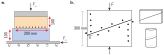
\includegraphics[scale=1]{../Figures_chap_etat/dispxp.pdf}
\caption[Deux types de presses mécaniques]{Schéma des deux méthodes d'application des forces normale et cisaillante. \textbf{a.}\,Application de la force cisaillante indépendamment de la force normale. La force normale est fixée, et la force cisaillante est pilotée par le déplacement du chariot (adapté de\,\cite{svetlizky_brittle_2019}). Dans le cas présent les carrés noirs symbolisent la position de jauges de déformation. \textbf{b.}\,Application d'une force unique sur une interface biseautée. L'angle du biseau $\alpha$ détermine la proportion de la force $F$ distribuée sur la normale et la tangente à l'interface (adapté de\,\cite{schubnel_photo-acoustic_2011}). Dans le cas présent les carrés noirs représentent la position de capteurs acoustiques et accélérométriques. Cette méthode d'application des forces peut être utilisée sur des plaques minces\,\cite{xia_laboratory_2004, nielsen_experimental_2010,mclaskey_foreshocks_2013, rubino_understanding_2017} ou sur des cylindres\,\cite{schubnel_photo-acoustic_2011,passelegue_sub-rayleigh_2013,passelegue_dynamic_2016}.}
\label{fig:dispxp}
\end{figure}

La presse mécanique a pour but de presser et cisailler les deux échantillons. Deux approches principales ont été mises en place. La première consiste en l'application d'une pression normale indépendamment de la force cisaillante, au moyen d'une presse purement normale et d'une platine de translation liée à l'extrémité d'un des blocs, tandis que l'autre est immobile\,\cite{rubinstein_detachment_2004,rubinstein_crack-like_2006,rubinstein_dynamics_2007,kammer_propagation_2012,kammer_slip_2014, svetlizky_classical_2014,svetlizky_brittle_2017,bayart_slippery_2016,svetlizky_brittle_2019} (Fig.\,\ref{fig:dispxp}a). Une variation de ce dispositif consiste en l'application de la force cisaillante directement sur le côté du bloc, dans toute sa hauteur\,\cite{rosakis_intersonic_2000,mclaskey_earthquake_2019}. La deuxième approche consiste en l'application d'une seule force sur les échantillons, sur une interface effectuant un angle relativement à cette force\,\cite{xia_laboratory_2004,nielsen_experimental_2010, schubnel_photo-acoustic_2011, latour_characterization_2013, mclaskey_foreshocks_2013, passelegue_sub-rayleigh_2013, passelegue_dynamic_2016,rubino_understanding_2017} (Fig.\,\ref{fig:dispxp}b). L'angle choisi est alors pris proche de l'angle critique pour lequel le mouvement de stick-slip peut avoir lieu, c'est à dire $\alpha_c =\arctan \mu_s$.



\subsubsection{Échantillons pressés}

Les échantillons choisis sont presque systématiquement des plaques minces, et occasionnellement des cylindres (études menées dans le groupe de F.\,X.\,Passelègue). Ce choix permet d'effectuer une hypothèse de planéité des contraintes, et donc de réduire le système étudié à deux dimensions. L'interface formée par ces plaques peut alors varier en longueur de l'ordre de quelques centimètres pour la plupart des études jusqu'à un ou plusieurs mètres (études menées dans les groupes de E.\,Fukuyama et G.\,C.\,McLaskey).

Les matériaux choisis diffèrent selon les études. Lorsque la portée de l'étude considérée est orientée vers la géophysique ou la mécanique des roches, ce sont des échantillons de roches qui sont choisis, comme par exemple du granite (études menées dans les groupes de E.\,Fukuyama, G.\,C.\,McLaskey et A.\,Schubnel).
%Ces roches ont cependant des inconvénients dans le cadre d'expériences nécessitant des propriétés mécaniques et optiques spécifiques. Pour cela des matières plastiques sont utilisées.
L'utilisation de roches présente cependant plusieurs inconvénients, tels que la grande vitesse de propagation des ondes acoustiques en leur sein ou les possibles hétérogénéités des échantillons.
Des matières plastiques sont utilisées afin de réduire la vitesse des ondes dans le milieu et d'assurer l'homogénéité de l'échantillon utilisé. Leur transparence permet également d'implémenter des mesures à l'interface par imagerie.
Deux catégories de plastiques polymères ressortent, les plastiques acryliques tels que le PMMA (études menées dans le groupe de J.\,Fineberg)\,\cite{rubinstein_detachment_2004,rubinstein_crack-like_2006,rubinstein_dynamics_2007, svetlizky_classical_2014,svetlizky_brittle_2017, bayart_slippery_2016, svetlizky_brittle_2019} et les plastiques polycarbonates tels que le PADC (homalite, études menées dans les groupes de A.\,J.\,Rosakis et A.\,Schubnel)\,\cite{rosakis_intersonic_2000, xia_laboratory_2004, latour_characterization_2013, nielsen_experimental_2010, schubnel_photo-acoustic_2011, rubino_understanding_2017}. Ces deux familles de matériaux ont des propriétés mécaniques proches, avec notamment un module d'Young de quelques gigapascals (contre plusieurs dizaines de gigapascals pour les roches).


En fonction des propriétés mécaniques et optiques des matériaux, plusieurs techniques de mesure sont implémentées sur ces systèmes.

\subsubsection{Dispositifs de mesure}


Les dispositifs de mesure utilisés pour déterminer les contraintes  à l'interface et mesurer la propagation de ruptures sont répartis en trois catégories (Fig.\,\ref{fig:dispmes}).

Tout d'abord les mesures peuvent être des mesures directes du tenseur des déformations sur les surfaces des échantillons, au moyen de jauges de déformation (études menées dans les groupes de J.\,Fineberg, G.\,C.\,McLaskey, A.\,Schubnel et M.\,Violay).
%\,\cite{rubinstein_detachment_2004,rubinstein_crack-like_2006,rubinstein_dynamics_2007,kammer_propagation_2012,kammer_slip_2014, svetlizky_classical_2014, svetlizky_brittle_2017, bayart_slippery_2016, svetlizky_brittle_2019, mclaskey_stress_2011, mclaskey_slow_2017}
Ces mesures permettent de déterminer directement le tenseur des déformations dans le bloc grâce à l'hypothèse de planéité des contraintes permise par leur géométrie.
%Elles nécessitent un dispositif d'acquisition électronique rapide doublé d'un système d'amplification électronique à faible bruit.

La transparence des matériaux plastiques permet d'utiliser des méthodes de mesure optique en imageant l'interface ou la surface des blocs au moyen d'une caméra rapide. L'interface peut être imagée par réflexion interne totale (TIR) afin de mesurer en temps réel la surface de contact réelle $A_r$ entre les deux blocs (études menées dans les groupes de J.\,Fineberg et G.\,C.\,McLaskey, Fig.\,\ref{fig:dispmes}a).
%\,\cite{rubinstein_detachment_2004,rubinstein_crack-like_2006,rubinstein_dynamics_2007,kammer_propagation_2012,kammer_slip_2014, svetlizky_classical_2014,svetlizky_brittle_2017,bayart_slippery_2016,svetlizky_brittle_2019}
Les propriétés photoélastiques du PADC pour leur part permettent de mesurer les déformations des blocs par les changements d'indice optique en transmission (études menées dans les groupes de S.\,Latour, S.\,Nielsen et A.\,J.\,Rosakis, Fig.\,\ref{fig:dispmes}).
%\,\cite{rosakis_intersonic_2000, xia_laboratory_2004}
D'autres mesures optiques sont possibles, telles que la mesure des déformations à la surface d'un bloc par des méthodes de corrélation d'images (DIC, études menées par les groupes de N.\,Lapusta et A.\,J.\,Rosakis)\,\cite{rubino_understanding_2017,buijze_nucleation_2020}. Il est enfin possible d'effectuer des mesures acoustiques des ondes se propageant dans le matériau
%\,\cite{nielsen_experimental_2010,schubnel_photo-acoustic_2011, passelegue_sub-rayleigh_2013}
(études menées dans le groupe de A.\,Schubnel, Fig.\,\ref{fig:dispmes}c). Ces mesures proches des mesures sismologiques permettent de déterminer la vitesse de propagation d'une rupture ou la position de l'épicentre d'un évènement grâce au contenu fréquentiel et au retard des ondes acoustiques émises.


Ces mesures diverses convergent vers un résultat similaire, qui est l'observation de la propagation de ruptures à l'interface frictionnelle.




\begin{figure}[p!]
\centering
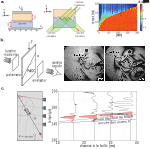
\includegraphics[scale=1]{../Figures_chap_etat/dispmes.pdf}
\caption[Présentations des différentes mesures]{Différentes méthodes de mesure de la propagation de rupture à l'interface. \textbf{a.}\,Mesure optique de la surface de contact réelle par réflexion interne totale.  (adapté de\,\cite{svetlizky_brittle_2019}). Deux plaques de PMMA sont pressées ($F_N=\SI{5500}{\newton}$) et cisaillées. Une réduction rapide de $A(x, t)$ a lieu au moment d'une chute de force cisaillante. La fracture se propage de gauche à droite, le temps est en ordonnée. Les portions d'interface dans lesquelles la fracture est déjà passée ont une aire de contact plus faible (bleu) que les régions encore intactes (rouge) \textbf{b.}\,Mesure optique des déformations par photoélasticimétrie dans un bloc de PADC au passage d'une rupture sub-Rayleigh (gauche) et supershear (droite) (adapté de\,\cite{xia_laboratory_2004}). Les déformations des plaques modifient l'indice optique extraordinaire $n_e$ de la plaque biréfringente, entraînant des variations de polarisation de la lumière. \textbf{c.}\,Mesure acoustique de la propagation d'une rupture (adapté de\,\cite{passelegue_sub-rayleigh_2013}). L'arrivée des ondes de compression sur les détecteurs permet de repérer l'avancée de la rupture. Dans le cas d'une rupture supershear, la même mesure peut s'effectuer par la détection du cône de Mach associé.}
\label{fig:dispmes}
\end{figure}

\subsection{Ruptures interfaciales}

\subsubsection{Observation des ruptures}



Au moyen des méthodes décrites ci-dessus, les études précédemment citées montrent que l'initiation d'un mouvement de glissement rapide au cours d'un cycle de stick-slip s'accompagne de la propagation d'une rupture dynamique à l'interface. Cette rupture consiste en l'affaiblissement des contacts frictionnels entre les blocs, comme montré par la réduction de la surface de contact réelle $A_r$ au moment de l'initiation du mouvement\,\cite{svetlizky_brittle_2019}. Il a été montré que ces ruptures peuvent être séparées en deux catégories en fonction de leur vitesse $v$. Les ruptures telles que $v<c_r$ la vitesse des ondes de Rayleigh dans le matériau considéré sont dites sub-Rayleigh. D'autres ruptures telles que $v>c_s$ la vitesse des ondes de cisaillement dans le matériau sont observées. Ces ruptures sont dites supershear, et du fait de leur vitesse supérieure à la vitesse des ondes dans le milieu, elles sont accompagnées d'un cône de Mach. Ces deux types de ruptures peuvent interagir, des études montrent en particulier qu'une rupture sub-Rayleigh peut déclencher une rupture supershear\,\cite{xia_laboratory_2004, schubnel_photo-acoustic_2011,passelegue_sub-rayleigh_2013}. La vitesse de ces ruptures est contrôlée par l'énergie élastique disponible au moment de leur initiation\,\cite{svetlizky_brittle_2017}.




\subsubsection{Simulation des ruptures}


La propagation de ruptures à l'interface frictionnelle a également été observée dans des simulations numériques de dispositifs similaires ou de systèmes minimaux\,\cite{radiguet_survival_2013, barras_study_2014, tromborg_slow_2014, amundsen_steady-state_2015, thogersen_minimal_2019}. Ces modèles permettent de rendre compte des phénomènes observés dans les systèmes expérimentaux décrits ci-dessus, comme la transition entre une rupture sub-Rayleigh et supershear\,\cite{passelegue_sub-rayleigh_2013,kammer_equation_2018, svetlizky_dynamic_2020}, mais également de phénomènes plus complexes tels que la robustesse de cette phénoménologie dans le cas d'interfaces formées par deux blocs de matériaux différents\,\cite{barras_study_2014,bar-sinai_slow_2012}.


\subsubsection{Description quantitative des ruptures}



\begin{figure}[htb]
\centering
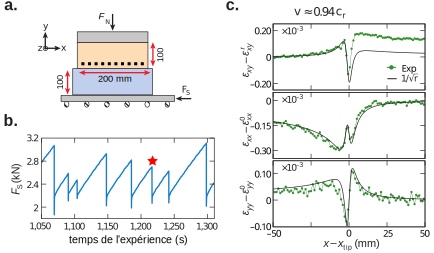
\includegraphics[scale=1]{../Figures_chap_etat/svet_propag.pdf}
\caption[Mesure des déformations associées à une rupture frictionnelle]{Mesure des déformations associées à une rupture frictionnelle (adapté de\,\cite{svetlizky_brittle_2019}). \textbf{a.}\,Dispositif expérimental. Deux plaques de PMMA ($c_r \simeq \SI{1250}{\meter\per\second}$) sont pressées l'une contre l'autre avec une force normale $F_N=\SI{5500}{\newton}$. \textbf{b.}\,L'interface subit un mouvement de stick-slip lorsque la force cisaillante $F_S$ augmente de manière quasi-statique. \textbf{c.}\,Mesures des variations du tenseur des déformations lors de l'évènement marqué d'une étoile rouge. Les prédictions LEFM sont tracées en noir, $\Gamma\simeq\SI{2.5}{\joule\per\meter\squared}$ est le seul paramètre libre.}
\label{fig:reflex}
\end{figure}


Dans le cas des ruptures sub-Rayleigh, il a été montré que les déformations qu'elles engendrent ainsi que leur propagation sont décrites par la mécanique de la fracture linéaire élastique (LEFM)\,\cite{kammer_linear_2015,svetlizky_brittle_2019} (Fig.\,\ref{fig:reflex}). La mesure des déformations à l'aide de jauges de déformation montre qu'au passage d'une rupture à l'interface, $\varepsilon_{xy}$ décroît d'une valeur initiale $\varepsilon_{xy}^0$ à $\varepsilon_{r}$, en effectuant une vaguelette (Fig.\,\ref{fig:reflex}). Cette vaguelette est caractéristique des ruptures LEFM, décrites par l'Équation\,\ref{eq:fracdynfric} pour un crack en mode\:\textsc{ii}. Il est notamment possible d'effectuer un ajustement du signal mesuré par les prédictions théoriques, avec pour seul paramètre libre l'énergie de fracture, ce qui donne un excellent accord. La dynamique des ruptures ainsi observées est également décrite par les équations de la théorie LEFM\,\cite{svetlizky_brittle_2017}.



Nous avons vu dans cette section que la caractérisation de la dynamique d'une interface frictionnelle solide-solide est bien comprise. Il est attesté que le mouvement de glissement s'amorce par le moyen de la propagation d'une rupture frictionnelle, aussi bien dans les matériaux plastiques que dans les roches. Cette rupture peut être mesurée par des techniques optiques, électromécaniques ou acoustiques. Dans le cas des ruptures sub-Rayleigh, il est même possible de la décrire au moyen de la théorie LEFM.


Les interfaces frictionnelles d'intérêt géologique sont cependant complexes de part leur géométrie, leur composition, et leur histoire, les menant à incorporer des hétérogénéités.


\section{Interface hétérogène}
\label{sec:hetero}


Nous appelons interface hétérogène une interface comportant dans sa longueur une hétérogénéité locale. Cette hétérogénéité peut consister en une différence de composition, par exemple la présence d'un patch de lubrifiant, de milieu granulaire, ou d'un matériau différent. Elle peut également consister en une altération mécanique ou géométrique de la surface de contact, comme la présence d'un trou, d'un état de surface différent, ou d'un défaut ou excès de chargement local. Les failles sismiques réelles sont hautement hétérogènes, et l'étude en laboratoire et la simulation d'hétérogénéités modèles permettent d'améliorer leur compréhension.

Nous présentons dans cette section les modifications de la dynamique d'une interface frictionnelle dues à la présence d'une hétérogénéité. Celle-ci peut agir comme une barrière à la propagation d'une rupture interfaciale ou comme une zone de glissement lent.





\subsection{L'hétérogénéité agit comme une barrière}
La propagation d'une rupture observée sur une portion d'interface peut ralentir ou s'arrêter à la rencontre de l'hétérogénéité. Ce phénomène est considéré comme pouvant être à l'origine de l'arrêt des séismes.

\subsubsection{Mécanismes d'arrêt}

\begin{figure}[htb]
\centering
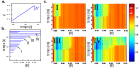
\includegraphics[scale=0.9]{../Figures_chap_etat/arrested.pdf}
\caption[Ruptures arrêtées]{Ruptures arrêtées par une inhomogénéité de contrainte, et donc d'énergie de rupture (adapté de\,\cite{rubinstein_dynamics_2007}). \textbf{a.}\,Mouvement de stick-slip à l'interface. \textbf{b.}\,Longueur des évènements de rupture. Les évènements I, II et III sont des ruptures arrêtées, tandis que l'évènement IV est une rupture traversant toute l'interface. \textbf{c.}\,Aire réelle de contact normalisée au cours des quatre évènements repérés. La faible aire de contact à l'extrémité gauche de l'interface correspond à une zone de faible énergie de fracture.}
\label{fig:moche}
\end{figure}





% La raison de l'arrêt de la propagation d'une rupture est le changement d'énergie de fracture. En effet si $\Gamma$ dépend de la position le long de l'interface, la propagation du crack ne s'effectue pas à vitesse constante (Éq.\,\ref{eq:propagfracdyn}). Une rupture initiée dans une région où $\Gamma$ est faible peut perdre en vitesse puis s'arrêter dans une région où $\Gamma$ est plus élevé. La rupture peut également être déviée, ou guidée par d'autres plans faibles que le plan principal de l'interface\,\cite{gudmundsson_effects_2010}.

% Un exemple de rupture arrêtée apparaît lors de l'introduction de lubrifiant sur une portion seulement de l'interface\,\cite{bayart_slippery_2016, bayart_rupture_2018}. Lorsqu'une rupture nuclée dans une portion de l'interface sans lubrifiant, elle peut être stoppée par la zone lubrifiée en raison de l'augmentation d'énergie de fracture qu'elle rencontre. En effet le critère de propagation $G=\Gamma$ (Éq.\,\ref{eq:propagfracdyn}) n'est plus vérifié en cas de changement soudain de $\Gamma$ à l'interface.



% La même phénoménologie apparaît lorsque la contrainte cisaillante appliquée n'est pas spatialement homogène (Éq.\,\ref{eq:homospa}), les fronts de rupture peuvent se propager sur une portion de l'interface et s'arrêter avant de briser l'ensemble de l'interface\,\cite{kammer_linear_2015,
%radiguet_survival_2013,
%rubinstein_dynamics_2007,
%scheibert_role_2010,
%bayart_rupture_2018,
%taloni_scalar_2015}. Ainsi un défaut de chargement dans une interface frictionnelle solide-solide peut mener à l'apparition de ruptures arrêtées, comme montré par Bayart et al.\,\cite{bayart_slippery_2016} (Fig.\,\ref{fig:moche}).Ces ruptures partielles de l'interface sont des précurseurs d'un mouvement de glissement macroscopique de l'interface, comparables aux \textit{foreshocks} des séismes de grande magnitude.


%Les ruptures arrêtées agissent également comme des hétérogénéités de contraintes par la concentration des contraintes qu'elles occasionnent en leur point d'arrêt. Cette situation est particulièrement pertinente dans le cadre de la prévention sismique, puisque les séismes ne sont jamais des ruptures de toute la longueur d'un système de faille, mais des ruptures arrêtées.



Une rupture peut dans certains cas être arrêtée par un changement d'énergie de fracture. En effet si $\Gamma$ dépend de la position le long de l'interface, la propagation du crack ne s'effectue pas à vitesse constante (Éq.\,\ref{eq:propagfracdyn}). Une rupture initiée dans une région où $\Gamma$ est faible peut s'arrêter dans une région où $\Gamma$ est plus élevé, le critère de propagation $G=\Gamma$ n'étant alors plus vérifié. Un exemple de rupture arrêtée apparaît lors de l'introduction de lubrifiant sur une portion seulement de l'interface\,\cite{bayart_slippery_2016, bayart_rupture_2018}. Lorsqu'une rupture nuclée dans une portion de l'interface sans lubrifiant, elle peut être stoppée par la zone lubrifiée en raison de l'augmentation d'énergie de fracture qu'elle rencontre.


La même phénoménologie peut apparaître lorsque la contrainte cisaillante appliquée n'est pas spatialement homogène (Éq.\,\ref{eq:homospa}), les fronts de rupture s'arrêtant alors avant de briser l'ensemble de l'interface\,\cite{kammer_linear_2015,
radiguet_survival_2013,
rubinstein_dynamics_2007,
scheibert_role_2010,
bayart_rupture_2018,
taloni_scalar_2015}. Ainsi un défaut de chargement dans une interface frictionnelle solide-solide peut mener à l'apparition de ruptures arrêtées, comme montré par Bayart et al.\,\cite{bayart_fracture_2016} (Fig.\,\ref{fig:moche}). Ces ruptures partielles sont des précurseurs d'un mouvement de glissement macroscopique de l'interface, comparables aux \textit{foreshocks} des séismes de grande magnitude. Les ruptures arrêtées agissent également comme des hétérogénéités de contraintes par la concentration des contraintes qu'elles occasionnent en leur point d'arrêt. Cette situation est particulièrement pertinente dans le cadre de la prévention sismique, puisque les séismes ne sont jamais des ruptures de toute la longueur d'un système de faille, mais des ruptures arrêtées.

La dynamique de la rupture peut également être affectée par les propriétés géométriques de l'interface. Elle peut être arrêtée, déviée, ou guidée par d'autres plans faibles que le plan principal de l'interface\,\cite{gudmundsson_effects_2010}, ou par la présence d'un milieu granulaire.





\subsubsection{Barrière granulaire}


L'hétérogénéité menant à l'arrêt de la propagation peut également consister en une inclusion de milieu granulaire à l'interface\,\cite{rubino_intermittent_2022,buijze_nucleation_2020,buijze_effects_2021}. Le mécanisme par lequel une inclusion de milieu peu cohésif interagit avec les portions solide-solide de l'interface reste mal compris, et reste généralement expliqué par les descriptions empiriques des modèles Rate-and-State. Rubino et al. ont par exemple observé par DIC des ruptures s’arrêtant dans une couche de gouge localisée, et l'ont attribué au comportement renforcé en vitesse de la gouge\,\cite{rubino_intermittent_2022}. Cette description coïncide avec celle proposée par Buijze et al. d'une interface entièrement granulaire hétérogène\,\cite{buijze_nucleation_2020}. Cette phénoménologie rapprocherait alors le patch granulaire d'un patch glissant, que nous décrivons dans la section suivante.

L'hétérogénéité peut être artificiellement créée, mais même lorsque qu'un milieu granulaire est initialement réparti à l'interface de manière homogène, des hétérogénéités émergent. En effet la formation d'une hétérogénéité peut être imputée à l'usure 
de l'interface. Dans le cas d'une interface de roches séparées par une poudre fine et homogène, la répartition de la poudre peut changer jusqu'à former des hétérogénéités de contraintes\,\cite{cebry_creep_2022, buijze_nucleation_2020,gvirtzman_nucleation_2021}. Dans le cas de Cebry et al., le système étudié, une interface de blocs plastiques encapsulant une fine couche de poudre de quartz, a naturellement évolué vers la formation de deux aspérités. Ces deux aspérités imposent alors une dynamique complexe à l'interface, entraînant une co-sismicité de ses différentes portions.

\subsubsection{Co-sismicité}
La co-sismicité est la manifestation d'un couplage entre deux failles sismiques. Lorsqu'une faille se rompt dans un évènement sismique, les contraintes qu'elle retenait sont relâchées, et redistribuées aux failles avoisinantes. Cette co-sismicité se retrouve dans des systèmes pour lesquels la rupture arrêtée par l'hétérogénéité entraîne la nucléation d'une autre rupture de l'autre côté de l'hétérogénéité, l'arrêt de la rupture reportant les contraintes libérées par la partie brisée sur la portion encore intacte de l'interface\,\cite{rubino_intermittent_2022}. La rupture arrêtée est alors un précurseur pour un évènement de rupture de l’interface entière.

Ces phénomènes soulèvent la question des mécanismes de couplage entre les différentes portions d'une faille. Ces mécanismes sont importants dans la compréhension des phénomènes de précurseurs et répliques (\textit{foreshocks and aftershocks}) des séismes\,\cite{felzer_common_2004}, ces ruptures arrêtées pouvant alors être des précurseurs de séismes de magnitude plus élevée. Au contraire après un séisme la zone déchargée peut agir comme une hétérogénéité de contrainte pouvant arrêter une rupture sismique déclenchée dans une portion de faille voisine, limitant ainsi l'amplitude des répliques.


Une hétérogénéité arrêtant une rupture peut être décrite dans le cadre des modèles Rate-and-State par la présence dans une interface d'un patch dont la dépendance du frottement en vitesse est différente de celle du reste de la faille\,\cite{chen_scaling_2009,schwartz_slow_2007,noda_stable_2013} (Sec.\,\ref{sec:rateandstate}). Cette description suppose cependant que la portion renforcée de l'interface glisse lentement lorsqu'elle est soumise à une contrainte cisaillante extérieure. Nous présentons par la suite des systèmes dans lesquels des portions de failles ne présentent pas d'activité sismique et relâchent les contraintes par le moyen d'un glissement lent.



\subsection{L'hétérogénéité est une zone en glissement lent}



Certaines portions de failles sismiques sont en mouvement lent, soit permanent, soit ponctuel au cours d'évènements de quelques minutes ou plus\,\cite{peng_integrated_2010,burgmann_geophysics_2018}. Le mécanisme responsable de ces phases de glissement reste encore méconnu, tout comme son rôle dans l'activité sismique d'une zone de failles\,\cite{radiguet_triggering_2016,dragert_silent_2001}. Dans cette section nous présentons ces zones de glissement, qui sont des hétérogénéités au sein d'une interface frictionnelle bloquée par ailleurs.


\subsubsection{Observation du glissement lent}

Les séismes lents ont d'abord été observés dans les zones de subduction, en particulier au Japon, situé au-dessus d'une des zones sismiques les plus actives du monde\,\cite{kanamori_mechanism_1972}. Ces observations d'abord indirectes\,\cite{sacks_slow_1978} ont mené à les nommer également séismes silencieux (\textit{silent earthquakes}) en raison de la faiblesse de leurs émissions acoustiques. Des méthodes de mesure directe ont permis d'observer ce phénomène dans de nombreuses régions de failles\,\cite{harris_large_2017}. Les techniques d'observation modernes reposent principalement sur l'usage de données GPS, permettant un suivi précis au centimètre près du mouvement de la croûte terrestre.

Les zones de glissement lent sont surveillées de près par de nombreuses équipes de recherche. Une partie de la littérature actuelle portant sur ces séismes lents consiste en la description d'une région spécifique, généralement après ou avant un évènement sismique majeur. Par exemple Ozawa et al.\,\cite{ozawa_coseismic_2011} décrivent les répliques et précurseurs du grand séisme de Tōhoku de 2011, de magnitude $M_w=9$, mesurés par des données GPS. Ces résultats sont ensuite agrégés dans des études sur de longues périodes ou des méta-études telles que celle de Schwartz et Rokosky\,\cite{schwartz_slow_2007}, montrant que le glissement lent est un phénomène généralisé présent entre autres tout autour de la ceinture de feu du Pacifique. Il a de plus été observé que ces zones de glissement lent peuvent correspondre à des hétérogénéités de composition au sein d'un système de failles. Des mesures par carottage dans certaines failles en glissement lent particulièrement peu profondes au large de la Nouvelle Zélande montrent notamment que les séismes lents sont induits par des régions de forte hétérogénéité mécanique, frictionnelle, pétrographiques et géométrique\,\cite{barnes_slow_2020}. Une hétérogénéité de composition peut se traduire par une hétérogénéité dans la dynamique de la faille.

Ainsi les zones de glissement sont extensivement observées, décrites et étudiées, pourtant Schwartz et Rokosky indiquent que malgré cette profusion d'études, les mécanismes à l'origine de leur glissement et leur influence sur les zones de failles bloquées «\,\textit{restent élusifs}\,». Ils sont souvent passés sous silence au profit d'une approche plus empirique basée sur des modèles Rate-and-State (Sec.\,\ref{sec:rateandstate}), dont les coefficients sont ajustés pour décrire des portions de failles spécifiques. L'étude en laboratoire de failles en glissement lent, au travers des expériences telles que celle que nous présentons dans cette thèse (Chap.\,\ref{sec:chaparticle}) ou de simulations numériques, permet d’améliorer notre compréhension de ces mécanismes, mais également des interactions entre les différentes portions d'un système de failles.



\subsubsection{Modélisation des failles glissantes}

\begin{figure}[htb]
\centering
\includegraphics[scale=1]{../Figures_chap_etat/buijze.pdf}
\caption[Effet d'une gouge hétérogène sur le stick-slip]{Mouvement de stick-slip au sein d'une interface comportant une gouge hétérogène cisaillée (extrait de\,\cite{buijze_effects_2021}). La gouge est pressée à une contrainte normale $\sigma_2$, et cisaillée à une contrainte $\tau^*$. L'hétérogénéité est constituée d'un patch de composition minéralogique différente pour chaque couleur de courbe. En orange la gouge est homogène. Les courbes bleue, verte et rouge correspondent à trois compositions différentes pour l'hétérogénéité. Le mouvement de stick-slip peut, en fonction de l'hétérogénéité choisie, disparaître, s'accélérer ou ponctuer un glissement permanent.}
\label{fig:buijze}
\end{figure}



La conception de failles sismiques en laboratoire permet de contrôler avec précision les propriétés des matériaux insérés à l'interface, et d'étudier les variations dans la dynamique de celle-ci avec les propriétés de l'hétérogénéité insérée\,\cite{bedford_fault_2022,buijze_effects_2021,kaproth_slow_2013}. Buijze et al. ont en particulier étudié l'influence d'une hétérogénéité pétrographique au sein d'une gouge pressée entre deux blocs de PMMA\,\cite{buijze_effects_2021}. La faille de laboratoire a alors exhibé une grande variété de dynamiques selon la gouge utilisée. Les exemples notables sont un mouvement de stick-slip particulièrement bien défini (Fig.\,\ref{fig:buijze}, courbe orange), et au contraire une mise en glissement permanent de l'interface toute entière (courbe bleue). L'hétérogénéité locale est alors responsable de la mise en glissement lent de toute l'interface.

Bedford et al. pour leur part montrent que l'insertion d'une gouge d'argile et de quartz à l'interface entre deux blocs de roche cisaillés mène à l'apparition, en fonction de la proportion d'argile ou de sa disposition, soit d'une instabilité de stick-slip, soit d'une mise en glissement lent\,\cite{bedford_fault_2022}. L'augmentation de la proportion d'argile entraîne un renforcement en vitesse de l'interface.



Ainsi une hétérogénéité locale à l'interface peut agir comme un patch glissant, menant à une modification de la dynamique globale de l'interface. Ce glissement lent est généralement étudié sous le prisme des modèles Rate-and-State. Cette analyse, bien qu'elle passe sous silence les mécanismes responsables du glissement, permet la modélisation d'un système de failles par un patchwork de zones dont les coefficients $A$ et $B$ sont choisis pour représenter des systèmes réels ou modèles, dans l'objectif de déterminer l'influence de ce patchwork sur la sismicité globale de la région d'intérêt.


\subsubsection{Rôle sismologique du glissement lent}

Les systèmes de failles sismiques sont fortement couplés. La rupture d'une portion de faille influence la dynamique de toute la faille par {co-sismicité}. Ainsi il a été montré que le glissement lent d'une portion de faille peut déclencher une rupture sismique\,\cite{radiguet_triggering_2016}, et inversement une rupture sismique peut débloquer des portions de failles avoisinantes, se mettant en glissement lent\,\cite{ozawa_coseismic_2011,chlieh_coseismic_2007}. Ce dernier mécanisme est adjacent à celui de l'apparition de répliques, séismes déclenchés par un premier évènement de rupture, généralement de plus faible magnitude que celui-ci.


Afin de décrire ces phénomènes des modèles Rate-and-State sont utilisés. De nombreuses simulations montrent que les portions de failles en glissement lent ont un rôle déterminant dans le comportement des failles\,\cite{lui_repeating_2016,noda_stable_2013,harris_large_2017,radiguet_survival_2013,chen_scaling_2009, romanet_fast_2018}. Lorsque ces simulations sont axées vers la description d'un système de failles réel, l'ajustement des paramètres $A$ et $B$ des portions de failles définies est un facteur clé de l'étude. Noda et Lapusta\,\cite{noda_stable_2013} montrent notamment en modélisant la zone de faille de Fukushima au Japon que le glissement lent de certaines portions de faille mène à la déstabilisation de portions pourtant théoriquement stables, car stabilisées par la vitesse. Chen et Lapusta\,\cite{chen_scaling_2009} effectuent une étude similaire en partant des propriétés d'une portion de la faille de San Andreas. Les implications de ces études vont pourtant au-delà de la description d'un système de failles précis.

Des simulations plus générales permettent d'étudier la co-sismicité dans des systèmes modèles, et d'en comprendre les mécanismes. Il a ainsi été montré que les transferts d'énergie élastique dans les failles modèles peuvent s'effectuer à grande distance, de l'ordre de \SI{600}{\kilo\meter} le long de la faille de San Andreas entre San Francisco et Los Angeles par exemple\,\cite{lui_repeating_2016}. À la recherche de la complexité minimale nécessaire à l’apparition de ces phénomènes, il a également été montré que la présence d'une hétérogénéité n'est pas nécessaire à l'émergence d'un tel couplage au sein de failles modèles, qui peut être déclenché par des effets géométriques\,\cite{romanet_fast_2018,liu_aseismic_2005}.


L'influence d'une hétérogénéité à l'interface sur le comportement macroscopique de celle-ci est due à la création d'une zone en glissement lent au sein de la faille. Cette zone agit comme une barrière à la propagation des ruptures, mais n'isole pas pour autant les portions de failles de part et d'autre du patch glissant. Au contraire la présence de ces hétérogénéités est responsable de phénomènes de co-sismicité et d'interactions à longue portée au sein de systèmes de failles.

Au cours de cette section nous avons présenté des hétérogénéités de composition formées par des milieux granulaires hétérogènes, la section suivante présente des études portant sur les interfaces frictionnelles entièrement granulaires homogènes.



\section{Interface entièrement granulaire homogène}

L'hétérogénéité d'une l'interface peut être médiée par l'insertion d'une couche de gouge entre deux blocs solides. La gouge est une roche broyée non cohésive située au cœur des failles, façonnée par l'usure des matériaux en contact cisaillant. Ses propriétés mécaniques sont celles d'un milieu granulaire très polydisperse, pressé et cisaillé par la roche. L'influence d'un tel milieu granulaire sur la dynamique d'une interface frictionnelle peut être étudiée en laboratoire grâce à l'utilisation de milieu granulaires modèles, pressés et cisaillés par des matériaux solides.


\subsection{Rhéologie granulaire}



Les expériences de rhéologie granulaire se focalisent sur les propriétés du milieu granulaire en lui-même. Ce milieu généralement polydisperse est pressé et cisaillé, par exemple dans une cellule de Couette. Il a été montré qu'un granulaire cisaillé peut exhiber un mouvement de stick-slip dont les évènements sismiques sont d'amplitude variable, indépendamment des propriétés mécaniques ou géométriques des grains\,\cite{anthony_influence_2005}. Les évènements de stick-slip observés reproduisent alors des lois phénoménologiques de distribution des moments sismiques telles que la loi de Gutenberg-Richter\,\cite{lherminier_continuously_2019,houdoux_micro-slips_2021,abed_zadeh_seismicity_2019} (Sec.\,\ref{sec:failles}). Ces observations sont cohérentes avec les résultats d'études numériques portant sur des systèmes analogues\,\cite{lieou_simulating_2017,laurenti_deep_2022}.


Ces systèmes sont rarement étudiés sous l'angle de la propagation d'une rupture. Les mesures effectuées sont généralement des mesures acoustiques à relativement basse fréquence. Des dispositifs tels que celui développé par l'équipe de O.\,Ramos permettent, au moyen de méthodes optiques basées sur la biréfringence des grains, de mesurer les propriétés frictionnelles au sein de l'interface, et en particulier les chaînes de forces dans le milieu granulaire\,\cite{lherminier_continuously_2019, daniels_photoelastic_2017,majmudar_contact_2005}. Ces expériences font état d'avalanches de réarrangements des grains et des chaînes de forces\,\cite{ramos_avalanche_2009,dahmen_simple_2011,bares_local_2017}, qui sont des phénomènes propagatifs. Leur lien avec la propagation d'une rupture frictionnelle reste indéterminé.

Le cisaillement effectué dans ces expériences l'est au travers de blocs solides de rigidité infinie en comparaison à celle des grains, ne permettant pas de couplage élastique qui est une composante essentielle des failles réelles.

\subsection{Couplage avec un solide élastique}

\begin{figure}[htb]
\centering
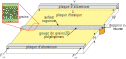
\includegraphics[scale=1]{../Figures_chap_etat/geller.pdf}
\caption[Dispositif expérimental d'étude d'une interface granulaire]{Exemple de dispositif utilisé pour coupler l'élasticité de blocs solides avec une interface granulaire (adapté de\,\cite{geller_stick-slip_2015}). Les grains polydisperses sont pressés et cisaillés à vitesse constante. La géométrie des plaques et des grains est choisie afin de permettre de considérer le système comme bidimensionnel ($H\ll L,W$).}
\label{fig:geller}
\end{figure}


Nous nous intéressons dans notre étude à des interfaces granulaires cisaillées par des solides élastiques. Ces systèmes permettent d'étudier le couplage entre l'élasticité des blocs et la dynamique du milieu granulaire, mais également de considérer que le milieu granulaire est une perturbation d'une interface solide-solide élastique (Fig.\,\ref{fig:geller}).

Le cisaillement par des blocs élastiques d'un milieu granulaire peut mener à une grande diversité de comportements. Il a été montré qu'un tel système peut avoir un mouvement de stick-slip mais également des phases de glissement permanent. Geller et al. montrent que le glissement des deux blocs séparés par un milieu granulaire épais est un glissement lent ponctué par des évènements rapides de chutes de force cisaillante\,\cite{geller_stick-slip_2015}. La distribution de ces chutes de force suit une loi de puissance type Gutenberg-Richter. L'expérience de Geller et al. est très similaire à des systèmes simulés tels que celui présenté par Zhang et al.\,\cite{zhang_two_2023}, qui s'en inspire. Les simulations numériques montrent un bon accord avec les expériences en laboratoire.

Lorsque le milieu granulaire est moins épais, ou évolue avec le temps, il peut perdre progressivement son homogénéité. Cebry et al.\,\cite{cebry_creep_2022} présentent par exemple un système dans lequel une gouge fine de quartz est cisaillée par deux blocs de PMMA. La gouge initialement homogène crée deux points de compressions de part et d'autre de l'interface. La dynamique de l'interface évolue alors au fil du cisaillement d'un glissement lent à une instabilité de stick-slip relativement régulière, puis à un comportement de plus en plus erratique. Cette étude soulève l'importance de l'usure de l'interface. D'autres expériences similaires montrent que l'interface, broyant la poudre qu'elle contient, se lubrifie par son usure dans un phénomène de lubrification solide\,\cite{reches_fault_2010}. Similairement au cas d'une interface solide-solide, des expériences et simulation ont montré que l'initiation du glissement s'accompagne de la propagation d'une rupture à l'interface\,\cite{cebry_creep_2022,buijze_nucleation_2020,buijze_effects_2021}. Cette rupture n'a cependant pas fait l'objet de caractérisations approfondies.
%et n'est a priori pas décrite par les loi de la mécanique de la fracture linéaire élastique.



\section{Objectifs de cette thèse}


Les objectifs de cette thèse sont tout d'abord de développer un dispositif expérimental complet pour notre étude. Ce dispositif doit permettre de presser et cisailler des plaques minces de PMMA encapsulant un milieu granulaire (Chap.\,\ref{sec:chapxp}). En particulier nous souhaitons implémenter des méthodes d'acquisition électronique pour la mesure du tenseur des déformations à haute fréquence permettant d'étudier la propagation de ruptures à l'interface (Sec.\,\ref{sec:electronique}); et des mesures par imagerie pour le suivi des grains (Sec.\,\ref{sec:optique}). Ce dispositif sera ensuite utilisé afin d'analyser la dynamique de plusieurs interfaces frictionnelles complexes incorporant des milieux granulaires. En particulier nous avons pour objectif l'étude d'une interface en œil granulaire (Chap.\,\ref{sec:chaparticle}), et d'une interface entièrement granulaire (Sec.\,\ref{sec:fullygranpersp}).


Par l'étude de ces interfaces nous voulons éclaircir les mécanismes de la friction granulaire à l'échelle microscopique. Pour ce faire nous souhaitons tout d'abord évaluer les modifications de la dynamique du système dues à la présence d'un milieu granulaire, notamment sur le mouvement de stick-slip à l'interface. Nous pourrons ensuite déterminer les mécanismes locaux responsables de ces modifications.

Dans le cas de l'œil granulaire nous nous intéressons en particulier au rôle d'un patch granulaire à l'interface dans la dynamique de glissement et sur l'initiation de ruptures frictionnelles. Les propriétés de cette interface la rapprochent de systèmes de failles de composition hétérogène. Nous espérons par cette étude améliorer la compréhension du couplage entre les portions glissantes et les segments bloqués au sein d'une faille. Dans le cas de l'interface entièrement granulaire, nous avons pour objectif d'étudier l'initiation du mouvement de glissement rapide à l'interface, et avons pour hypothèse qu'elle est médiée par la nucléation et la propagation d'une rupture frictionnelle dans le milieu granulaire. Cette étude permettra une meilleure compréhension du rôle de la gouge de faille dans les mécanismes sismiques.




En résumé, notre étude porte sur les interfaces frictionnelles perturbées par un milieu granulaire. En particulier nous nous intéressons à une interface bidimensionnelle en cisaillement, contenant des grains soit dans toute sa longueur, se rapprochant alors du dispositif expérimental présenté Figure\,\ref{fig:geller}, soit dans un espace restreint rendant l'interface hétérogène, comme présenté en Section\,\ref{sec:hetero}. Elle s'inscrit dans la continuité de l'étude des interfaces frictionnelles solide-solide et de la description de l'initiation du mouvement par la propagation d'une rupture, et vise à déterminer la robustesse de cette description à des perturbations telles que l'inclusion d'un milieu granulaire.



















\chapter{Développement expérimental}
\label{sec:chapxp}
\vspace*{-1cm}
Dans ce chapitre, nous détaillons le dispositif expérimental développé au cours de cette thèse. Le chapitre se divise en 4 sections, présentant le dispositif mécanique et les matériaux utilisés, puis les mesures électroniques et optiques implémentées sur le système.


\minitoc
\newpage

\section{Principe de l'expérience}
\label{sec:grossepresse}
\vspace{.5cm}

L'objectif du dispositif que nous avons développé est de permettre la compression et le cisaillement contrôlés de deux plaques minces de polyméthacrylate de méthyle (PMMA) de \qtyproduct[product-units=single]{150 x 80 x 10}{\mm} l'une sur l'autre. La compression s'effectue à position verticale imposée, et à force normale mesurée. Le cisaillement s'effectue à vitesse constante, et à force cisaillante mesurée. La force normale typique appliquée est de l'ordre de \SI{3000}{\N}, et le cisaillement est appliqué à une vitesse typique de \SI{20}{\micro\metre\per\second}. Le déplacement horizontal total imposé lors d'une expérience est typiquement de 6 à \SI{12}{\mm}, soit un temps d'expérience allant de 5 à 10 minutes.


\subsection{Presse mécanique}

Nous avons développé en partenariat avec Marc Moulin du Service d'Ingénierie Mécanique de l'ENS de Lyon une presse mécanique verticale contrôlée en position (Fig.\,\ref{fig:presse}).
Le déplacement vertical du bloc supérieur et l'application de la force normale se font par le biais d'une barre horizontale rigide équipée d'un capteur de force. Son déplacement, contrôlé en position par la rotation d'une vis, s'effectue par roulement sur des rails verticaux. Des patins rigides permettent un verrouillage de la position de la barre sur ces rails. Le déplacement tangentiel du bloc inférieur et l'application de la force cisaillante se font au moyen d'une platine de translation horizontale motorisée. Elle permet de translater le bloc inférieur tandis que le bloc supérieur reste fixe. Le bloc supérieur est
%disposé sur une platine de translation à roulement à billes 
solidaire d'un capteur de force, permettant la mesure de la force cisaillante exercée sur l'interface. Les échantillons pressés sont fixés au dispositif au moyen de mors métalliques dans lesquels ils sont encastrés d'un centimètre.

Du fait de la flexibilité des éléments mécaniques et de la géométrie du système, une faible rotation s'applique au bloc du haut lorsque le chargement cisaillant est appliqué. Pour compenser cette rotation, un système de vis permet d'assurer l'alignement des faces des deux blocs en contact, et d'homogénéiser les contraintes à l'interface.






\subsection{Mesure de force}

Deux capteurs de force sont installés sur la presse (Fig.\,\ref{fig:captforce}). La mesure de force par ces capteurs commerciaux repose sur une mesure des déformations engendrées par l'application d'une pression sur leurs faces par des jauges de déformation.
Les faces du capteur de force normale sont à cet effet solidaires respectivement de la vis de contrôle de la presse et de la barre horizontale, elle-même solidaire du bloc supérieur. Cette disposition permet à la vis d'appliquer la force normale sur le capteur, qui la retransmet à la barre, et donc à l'interface. Les faces du capteur de force cisaillante sont pour leur part solidaires respectivement de la barre horizontale et d'une platine de translation sans frottements à roulements à billes, sur laquelle est fixé le bloc supérieur. La force cisaillante, appliquée sur l'interface par la platine motorisée déplaçant le bloc inférieur, est alors retransmise au capteur par le biais de la platine de translation sans frottements.

Les déformations des capteurs sont négligeables devant celles des blocs ($E_\text{acier}\sim\SI{200}{\giga\pascal}\gg E_\text{PMMA}$), et ne perturbent pas le système mécanique étudié. Leur réponse en tension est une fonction affine de la force appliquée sur leurs extrémités. Ils peuvent mesurer des forces allant jusqu'à  $10^4\,\unit{\N}$, avec une précision de \SI{10}{\N}, et une bande passante de l'ordre d'un kilohertz.


\newpage

\begin{figure}[h!]
\centering
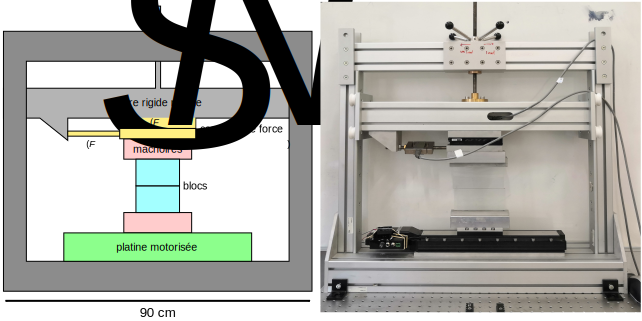
\includegraphics[scale=1]{../Figures_chap_exp/frame.pdf}
\caption[Schéma de la presse mécanique]{La presse est composée d'un cadre rigide (gris sombre), d'une barre horizontale mobile (gris clair), et d'une platine de translation commerciale (vert). La barre est installée par des poulies à gorge avec roulements à billes dans un guide limitant les rotations indésirables (roulis, tangage et lacet), et sa position est contrôlée manuellement par une vis. La platine de translation est contrôlable en position et en vitesse, pouvant aller de \SI{1}{\micro\meter\per\second} à \SI{10}{\mm\per\second}, sur une course de \SI{300}{\mm}. Des capteurs de forces (orange) permettent la mesure des forces normale et cisaillante appliquées à l'interface. Le dispositif est fixé par sa base sur une table optique.}
\label{fig:presse}
\end{figure}

\begin{figure}[h!]
\centering	
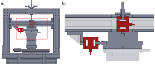
\includegraphics[scale=1]{../Figures_chap_exp/coupes_solidworks.pdf}
\caption[Disposition des capteurs de force]{\textbf{a.}\,Position des capteurs de force, en rouge, sur le cadre de la presse. Le capteur de force cisaillante est à gauche, le capteur de force normale est inséré dans la barre de translation verticale. \textbf{b.}\,Coupe transversale du cadre rouge. La force normale est appliquée sur l'interface au moyen d'une vis contrôlée manuellement, pressant sur le capteur de force. La force cisaillante est appliquée par le bloc inférieur, au moyen d'une platine de translation horizontale, et est retransmise au capteur de force cisaillante au moyen d'une platine à roulements à billes.}
\label{fig:captforce}
\end{figure}

\newpage


\section{Échantillons étudiés}
\label{sec:echantillons}

Nous avons étudié différents types d'interfaces frictionnelles, faisant intervenir des blocs solides et un système granulaire modèle, composés de matériaux plastiques.

Les blocs pressés sont des plaques fines de polyméthacrylate de méthyle de 80 mm de hauteur, formant une interface quasi bidimensionnelle de \qtyproduct[product-units=single]{150 x 10}{\mm}. Le milieu granulaire étudié est constitué de cylindres de nylon, de diamètre compris entre 0.4 et \SI{1.3}{\mm}, disposés dans la largeur de l'interface pour former un milieu granulaire 2D.

Cette section détaille les propriétés mécaniques des matériaux choisis pour les blocs et pour le milieu granulaire, ainsi que les géométries retenues pour notre étude.


\subsection{Blocs solides}

\subsubsection{Choix du matériau}
\label{sec:materials}

Le choix du matériau composant les plaques s'est fait sur le critère de la faible vitesse des ondes sonores en son sein, et donc de sa faible rigidité. En effet une plus grande rigidité implique une plus grande vitesse des ondes ($c_p\propto\sqrt{E/\rho}$), et impose une plus grande vitesse d'acquisition pour étudier les phénomènes propagatifs à l'interface. Pour autant nous utilisons un matériau suffisamment rigide pour ne pas atteindre son seuil de flambage. Notre choix s'est donc porté sur un matériau plastique rigide, le polyméthacrylate de méthyle (PMMA, ou \textit{Plexiglas}). Étant un matériau viscoélastique, son module d'Young $E$ dépend de la vitesse à laquelle il subit les déformations qui lui sont appliquées (il est dit \textit{strain rate dependent}\,\cite{mulliken_mechanics_2006}). Ainsi $E$ est compris entre 3.5 et \SI{5.6}{\giga\pascal} respectivement à faible et grande vitesse de sollicitation.

Afin de mesurer le module d'Young à l'aide de la presse, nous avons appliqué une force pressante sur un bloc de PMMA équipé de capteurs de déformation. Les mesures simultanées des déformations normale $\varepsilon_{yy}$ et orthogonale $\varepsilon_\perp$, et de la force normale $F_N$ appliquée sur la surface $A$ permettent de calculer $E$ et $\nu$ par un ajustement de la loi de Hooke (Fig.\,\ref{fig:fitE}). En effet $\sigma_{yy} = {F_N}/{A}=E\times\varepsilon_{yy}$ et $\nu = -{\varepsilon_\perp}/{\varepsilon_{yy}}$ (Sec.\,\ref{sec:hook}). Pour les chargements quasi-statiques, la valeur de $E$ mesurée et retenue est de \SI{3.5}{\giga\pascal}. Son coefficient de Poisson est $\nu = 0.3$. La vitesse des ondes de Rayleigh en son sein est $c_r\approx\SI{1250}{\meter\per\second}$. En référence, dans les métaux $E\approx\SI{100}{\giga\pascal}$ et $c_r\approx\SI{5000}{\meter\per\second}$, et dans les roches granitiques, $E\approx\SI{50}{\giga\pascal}$ et $c_r\approx\SI{2000}{\meter\per\second}$.

\begin{figure}[h!]
\centering	
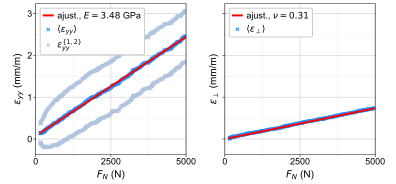
\includegraphics[scale=1]{../Figures_chap_exp/fit_E.pdf}
\caption[Mesure de $E$]{Mesure des propriétés mécaniques du PMMA. Le bloc de PMMA utilisé mesure \siprod{60 x 25 x 25}{\mm}, et est équipé de capteurs de déformation. La présence de deux capteurs de déformation sur des faces opposées permet de contrer leur non-parallélisme en effectuant la moyenne des deux mesures, c'est à dire $\left\langle\varepsilon_{yy}\right\rangle=(\varepsilon_{yy}^1+\varepsilon_{yy}^2)/2$.}
\label{fig:fitE}
\end{figure}






\subsubsection{Géométrie des blocs lisses}

La forme générale retenue pour les blocs est celle d'un parallélépipède de \siprod{150 x 80 x 10}{\mm}, en contact sur la tranche de \siprod{150 x 10}{\mm}. Les plaques sont rendues solidaires de la presse par le moyen de mors en acier de \SI{10}{\mm} de profondeur, ce qui réduit leur hauteur effective.

L'épaisseur du bloc a été choisie de \SI{10}{\mm}, faible devant ses deux autres dimensions, afin de pouvoir considérer l'échantillon comme bidimensionnel. Cette géométrie permet d'appliquer les simplifications associées à l'hypothèse de planéité des contraintes (\textit{plane stress}), et ainsi de restreindre le tenseur des déformations à deux dimensions et à trois composantes indépendantes. La face de contact a été dressée à la fraiseuse puis poncée manuellement avec du papier abrasif fin (P1200). La rugosité de surface de l'interface de contact est estimée à \SI{1}{\micro\meter} r.m.s. La planéité de la surface est de l'ordre de \SI{20}{\micro\meter}, mesurée avec un profilomètre confocal (Fig.\,\ref{fig:profilobloc}).


\begin{figure}[h]
\centering	
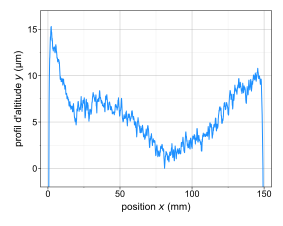
\includegraphics[scale=1]{../Figures_chap_exp/profil_bloc.pdf}
\caption[Profil moyen d'un bloc de PMMA]{Profil d'altitude moyen d'un des blocs pour l'étude d'une interface solide-solide, mesuré à l'aide d'un profilomètre confocal. La différence d'altitude entre le point le plus haut et le plus bas est de l'ordre de \SI{20}{\micro\meter} sur tous les blocs.}
\label{fig:profilobloc}
\end{figure}


\subsubsection{Géométrie des blocs granulaires}

\label{sec:geometriedesblocs}

Afin de solidariser le milieu granulaire aux blocs, le bord de ces derniers est percé d'alvéoles dans lesquelles des grains sont encastrés et collés (Fig.\,\ref{fig:blocgran}). Deux géométries sont alors utilisées dans notre étude, l'une que nous nommons l'interface en \textit{œil granulaire} et l'autre l'interface  \textit{entièrement granulaire}.


\myparagraph{Interface en œil granulaire}

L'interface en œil granulaire est composée de trois portions d'interface, deux portions solide-solide de 60 mm de long de part et d'autre d'un œil de longueur $\ell_{eye} = \SI{30}{\mm}$ contenant le milieu granulaire (Fig.\,\ref{fig:blocgran}a). L'œil est formé par deux cavités semi-elliptiques usinées dans chacun des blocs en contact, à la surface desquelles sont encastrés des grains de \SI{1.3}{\milli\meter} de diamètre tous les \SI{3}{\mm}. L'œil permet d'encapsuler un nombre variable de grains, faisant ainsi varier la densité du milieu. Le motif utilisé pour repérer optiquement les cylindres (Sec.\,\ref{sec:paint}) est reproduit en plusieurs points le long des portions solide-solide des blocs de part et d'autre de l'interface (Fig.\,\ref{fig:blocgran}c) afin de permettre des mesures de glissement interfacial (Sec.\,\ref{sec:suividesgrains}).


\pagebreak



\myparagraph{Interface entièrement granulaire}

L'interface entièrement granulaire est composée de grains dans toute sa longueur, encastrés dans le PMMA, soit à intervalle régulier, soit à intervalles aléatoirement générés, selon le bloc. Deux stoppeurs en silicone aux extrémités des deux blocs permettent de retenir une couche de grains d'épaisseur variable (\ref{fig:blocgran}b).




%\begin{figure}[h!]
\begin{figure}[htb]
\centering	
%\rule{0.6\textwidth}{0.4\textwidth}
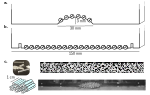
\includegraphics[scale=1]{../Figures_chap_exp/bloc_type_1.pdf}
\caption[Schéma des interfaces granulaires]{\textbf{a.}\,Interface à œil granulaire. L'œil granulaire mesure \SI{30}{\mm} de large par \SI{6}{\milli\meter} de hauteur et permet d'encapsuler une centaine de grains. \textbf{b.}\,Interface entièrement granulaire. Les grains encastrés à la surface du bloc sont espacés de 3 à \SI{8}{\milli\meter}, et peuvent être de diamètres variables. Les échelles ne sont pas respectées. \textbf{c.}\,Les grains sont disposés manuellement dans un arrangement aléatoire désordonné sur l'interface. Le motif peint sur les faces permet un suivi vidéo par corrélation d'images de la position et de la rotation de chaque grain, à une précision de l'ordre de \SI{5}{\micro\meter}.}
\label{fig:blocgran}
\end{figure}




\subsection{Milieu granulaire}

\myparagraph{Géométrie des grains}

Afin de conserver la structure quasi-bidimensionnelle du système, les grains sont des cylindres d'une longueur de \SI{10}{\milli\meter}, égale à la largeur de l'interface. Nous avons choisi des cylindres de différents diamètres (0.4, 0.7, 0.9 et \SI{1.3}{\milli\meter}) agencés parallèlement (Fig.\,\ref{fig:blocgran}c). La polydispersité des diamètres des grains permet d'éviter une cristallisation du milieu granulaire, qui modifierait ses propriétés mécaniques.




\myparagraph{Matériau des grains}

Les grains sont composés de Nylon ($E=\SI{1.4}{\giga\pascal}$, vérifié à l'aide d'une machine de traction, et $\nu=0.4$, tabulé), choisi pour ses propriétés mécaniques similaires à celles du PMMA composant les blocs. La proximité des modules d'Young des deux matériaux permet d'assurer un couplage entre l'élasticité de l'interface et celle des blocs.

Les cylindres sont réalisés à partir de fils de pêche de différents diamètres (0.4, 0.7, 0.9 et \SI{1.3}{\milli\meter}). Les fils sont redressés par la suspension d'une masse importante dans une étuve durant plusieurs heures. Une fois redressés ils sont manuellement coupés à la longueur voulue (\SI{10}{\milli\meter}) à l'aide d'une
%\href{https://youtu.be/hH5V2uqiSXc}{\textcolor{black}{guillotine}}
guillotine. Un motif est ensuite peint sur les deux faces circulaires des cylindres afin de faciliter le suivi des grains par imagerie (Sec.\,\ref{sec:paint}). L'état de surface du fil de nylon dans sa longueur n'est pas altéré.



Le système mécanique et les matériaux utilisés pour les échantillons ainsi définis, notre objectif est de mesurer les déformations des plaques minces de PMMA (\siprod{150 x 80 x 10}{\mm}, $E=\SI{3.5}{\giga\pascal}$) et les déplacements des grains de Nylon cylindriques (de diamètres allant de $0.4$ à \SI{1.3}{\mm}), afin de caractériser le comportement des différentes interfaces (surface lisse, entièrement granulaire ou en œil granulaire) que nous souhaitons étudier. Pour ce faire, nous avons développé un système de mesure électronique, reposant sur l'utilisation de jauges de déformation, et un système optique utilisant des méthodes de suivi par corrélation d'image.





\section{Mesures Électroniques}
\label{sec:electronique}

Afin de caractériser les efforts macroscopiques appliqués sur l'interface et leur répartition locale, ainsi que la dynamique des ruptures associées aux évènements de glissement, nous avons développé un système électronique permettant de mesurer les déformations des blocs et les forces pressante et cisaillante qui leur sont appliquées.

Le système électronique que nous avons développé, en partenariat avec Pascal Metz et Julian Miniot du Service d'Ingénierie Électronique du Laboratoire de Physique à l'ENS de Lyon, est une évolution du circuit développé dans le groupe de J. Fineberg (Hebrew University of Jerusalem).
Il permet d'amplifier et d'acquérir 60 voies de tension simultanément. Il combine des rafales d'acquisition rapide de \SI{10}{\milli\second} à \SI{4}{\mega\hertz}, déclenchées par un signal accélérométrique, et une acquisition lente à \SI{315}{\hertz} pouvant durer plusieurs dizaines de minutes. Il nous permet d'acquérir le signal de jauges de déformation, fournissant ainsi une mesure du tenseur des déformations 2D en 20 points le long de l'interface, ainsi que le signal des capteurs de forces normale et cisaillante, et du détecteur d'évènements accélérométrique.

Cette section détaille le dispositif de mesure des déformations et des forces, et de détection d'évènements.


\subsection{Mesure du tenseur des déformations}

La connaissance complète du tenseur des déformations 2D $[\varepsilon]$ permet de déterminer de nombreuses informations, telles que la répartition de la charge le long de l'interface, la vitesse et la direction de propagation des ondes, et les propriétés des ruptures interfaciales\,\cite{svetlizky_brittle_2017}. Ainsi mesurer $\varepsilon$ avec précision et à haute fréquence est l'objet principal du développement électronique que nous avons effectué. Sa mesure repose sur l'utilisation, le conditionnement, l'amplification et l'acquisition du signal de jauges de déformation.

\subsubsection{Jauge de déformation}
\label{sec:gages}

\myparagraph{Fonctionnement}

Une jauge de déformation est une feuille métallique de résistance connue, disposée en forme de créneau, intégrée dans une matrice en matériau isolant (Fig.\,\ref{fig:jauge}a). Elle est installée à l'aide d'un adhésif spécifique qui solidarise la matrice à la surface de l'échantillon étudié. Cette colle permet à toutes les déformations de l'échantillon d'être retransmises à la résistance, qui se déforme avec le bloc et voit sa valeur changer.

La variation de résistance est reliée à la déformation mécanique qu'elle subit dans son axe, notée $\varepsilon_{\parallel}$, par une loi polynomiale. Cette loi est généralement tronquée en une réponse linéaire par un coefficient $GF$ nommé \textit{facteur de jauge}, d'une valeur typique de l'ordre de 2, selon l'équation suivante, où $R_r$ est la résistance de la jauge au repos, et $\delta R$ est l'écart à cette valeur :

\begin{equation}
\label{eq:jauge}
\dfrac{\delta R}{R_r} = GF\times \varepsilon_{\parallel}
\end{equation}

Ainsi la mesure d'une déformation uni-axiale consiste en la mesure précise des variations d'une résistance.



Les jauges que nous utilisons sont agencées en rosettes à trois jauges (Fig.\,\ref{fig:jauge}b), écartées d'un angle de \ang{45}, de résistance \SI{350 +- 2}{\ohm}, et de facteur de jauge $GF=1.86$ pour les deux jauges latérales de la rosette, et $GF=1.79$ pour la jauge centrale de la rosette.



\begin{figure}[htb]
\centering	
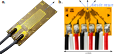
\includegraphics[scale=1]{../Figures_chap_exp/jauges.pdf}
\caption[Jauge de déformation]{\textbf{a.}\,Une jauge de déformation uni-axiale. Un allongement (respectivement une contraction) de sa matrice dans le plan provoque un allongement et un affinement par contraction de Poisson (resp. raccourcissement et épaississement) de la feuille métallique. Ces deux effets entraînent une augmentation (resp. diminution) de la valeur de la résistance. \textbf{b.}\,Trois jauges disposées en rosette, modèle utilisé dans notre étude. Lorsqu'une mesure bidimensionnelle du tenseur des déformations est requise, les jauges sont agencées en rosette dans une même matrice, permettant ainsi d'obtenir les trois composantes du tenseur 2D.}
\label{fig:jauge}
\end{figure}


\myparagraph{Nécessité d'amplifier -  calcul d'ordre de grandeur}

La variation de résistance $\delta R$ induite par les déformations du bloc est très faible par rapport à la valeur de résistance au repos $R_r$ de la jauge. Un calcul d'ordre de grandeur de la valeur de $\delta R$ dans le cadre typique de notre étude permet de déterminer la précision requise pour mesurer le signal de la jauge de déformation.

Prenons une force constante de 3000 N appliquée sur une interface de $150\times10$ mm, soit une surface \SI{1.5e-3}{\square\meter}, dans un bloc de PMMA de module d'Young $E=\SI{4}{\giga\pascal}$, parallèlement à l'axe d'une jauge de déformation de résistance $R_r=\SI{350}{\ohm}$ et de facteur de jauge $GF=2$. Alors la contrainte est donnée par
$\sigma_{\parallel} = {F_N}/{A} = \SI{2}{\mega\pascal}$. La loi de Hooke stipule que $\sigma_{\parallel}=E\varepsilon_{\parallel}$, donnant $\varepsilon_{\parallel} = \qty[per-mode = symbol]{5e-4}{\meter\per\meter}$. Enfin $\delta R/R_r = GF\times \varepsilon_{\parallel}$ permet de retrouver $\delta R =\SI{350}{\milli\ohm}$. Pour mesurer la composante continue du tenseur des déformations à \SI{10}{\percent} près, il faut donc pouvoir résoudre une valeur constante de l'ordre de \SI{10}{\milli\ohm}.

Si maintenant l'on considère une rupture typique issue de la théorie de la Mécanique de la Fracture Élastique Linéaire (LEFM, Sec.\,\ref{sec:LEFM}) d'énergie de rupture $\Gamma=\SI{1}{\joule\per\meter\squared}$, une vitesse de \SI{500}{\meter\per\second}, et des jauges installées à \SI{3}{\milli\meter} de l'interface, et que l'on calcule la variation typique de $\varepsilon_{\parallel}$ à son passage, nous trouvons que $\delta\varepsilon_{\parallel}\approx\qty[per-mode = symbol]{5e-5}{\meter\per\meter}$, et une variation de résistance associée de $\delta R = \SI{35}{\milli\ohm}$. Ainsi nous avons besoin d'une résolution de l'ordre du milliohm pour mesurer l'évolution de la composante variable du tenseur des déformations à $10^{-5}\,\text{m}/\text{m}$ près.

Pour mesurer ces faibles variations plusieurs approches existent, mais toutes sont équivalentes à mesurer une variation de la tension $U$ aux bornes de la jauge à intensité $I$ fixée. En notant $U=U_r+\delta U$, avec $U_r=R_r\times I$, sous obtenons

\begin{equation}
\delta U = \delta R\times I = GF\times R_r\times I\times \varepsilon_{\parallel}
\label{eq:1.2}
\end{equation}

Plus l'intensité sera élevée, plus les variations de tensions $\delta U$ seront élevées. 


Cependant les jauges étant des conducteurs ohmiques, elles dissipent une puissance $\mathcal{P}=U\times I=R I^2$ en chaleur, et peuvent fondre si cette chaleur n'est pas évacuée suffisamment rapidement. Le choix d'un matériau plastique, de faible conductivité thermique, limite grandement cette possibilité de dissipation ($\lambda_{\mathrm{PMMA}}\approx \SI{0.2}{\watt\per\meter\per\kelvin}$, en comparaison pour un matériau métallique $\lambda_{\mathrm{metal}}\sim 10^2\,\unit{\watt\per\meter\per\kelvin}$). La puissance dissipable est au maximum de \SI{1}{\milli\watt}, ce qui correspond à un courant d'intensité $I=\SI{1.7}{\milli\ampere}$.

La différence d'échelle entre la tension au repos $U_r$ et la variation de tension $\delta R$ soulève une autre difficulté. En effet à cette intensité de courant $U_r\approx\SI{0.6}{\volt}$, et si l'on conserve le critère de résolution de $10^{-5}$ m/m pour le tenseur des déformations, $\delta U\approx\SI{1}{\micro\volt}$. Ainsi une tentative d'amplification directe du signal de jauge est impossible, puisque l'amplification de la composante continue écraserait le signal à mesurer.

Pour mesurer cette tension, la technique expérimentale la plus couramment utilisée est le conditionnement par un pont de Wheatstone. Bien que nous ayons décidé à terme de ne pas utiliser de pont de Wheatstone dans le conditionnement de nos jauges de déformation mais une amplification par boucle d'Anderson, la présentation de ce montage permet d'en comprendre les avantages et les limites, et de justifier notre choix.

\subsubsection{Conditionnement traditionnel par pont de Wheatstone}


Un pont de Wheatstone est un circuit électrique pouvant être utilisé pour déterminer la valeur d'une résistance électrique inconnue, et pour mesurer avec précision ses fluctuations autour d'une valeur d'équilibre. Ce montage permet non seulement de mesurer avec précision la résistance d'une jauge, mais aussi ses variations autour de son état au repos, dans la limite de faibles écarts.



\begin{figure}[htb]
\centering	
\includegraphics[scale=1]{../Figures_chap_exp/Wheatstonebridge.pdf}
\caption[Pont de Wheatstone]{Montage d'un pont de Wheatstone en configuration quart-de-pont. Une des résistances du pont est une jauge de déformation, tandis que les trois autres sont des résistances fixes de valeur $R=R_r$ égale à la résistance au repos de la jauge. En pratique, afin de pallier aux variations de résistance des composants autour de leur valeur nominale et d'équilibrer le pont, la résistance $R_{\mathrm{BD}}$ est un potentiomètre. La tension $U_{\mathrm{AB}}$ est fixée constante, et la tension mesurée est la tension $U_{\mathrm{CD}}$.}
\label{fig:wheatstone}
\end{figure}


\myparagraph{Principe}


 En utilisant le théorème de Millman sur le montage présenté (Fig.\,\ref{fig:wheatstone}) nous obtenons
 
\begin{equation}
U_{\mathrm{CD}} = U_{\mathrm{AB}}
	\times
\dfrac{\delta R}{4R_r}
	\times
\left(
	\dfrac{1}{1+\frac{\delta R}{4R_r}}
\right)
\end{equation}

De plus, la fonction $f$ qui à $x$ associe $f(x)=\dfrac{1}{1+x}$ étant de classe $\mathcal{C}^\infty$ autour de 0, le théorème de Taylor-Young assure qu'il existe un développement limité de cette fonction en 0, et que ce développement limité prend la forme

\begin{equation}
f(x) = f(0) + f'(0)\times x + \dfrac{f''(0)}{2!}\times x^2 +\dots+  \dfrac{f^{(n)}(0)}{n!}\times x^n  + o(x^n)
\end{equation}

Étant donné que dans les conditions normales d'utilisation d'une jauge de déformation ${\delta R}/{4R_r}$ est proche de 0,  nous pouvons appliquer ce développement limité à $U_{\mathrm{CD}}$, avec $x={\delta R}/{4R_r}$ et $n=3$, ce qui donne

\begin{equation}
U_{\mathrm{CD}}= \dfrac{U_{\mathrm{AB}}}{4}
	\times
\left[
	\dfrac{\delta R}{R_r}
		-
	\dfrac{1}{4}\left(\dfrac{\delta R}{R_r}\right)^2
		+
	\mathcal{O}
		\left(
			\left(\dfrac{\delta R}{R_r}\right)^3
		\right)
\right]
\end{equation}

Et en utilisant la relation résistance-déformation d'une jauge (Éq.\,\ref{eq:jauge}) il vient

\begin{equation}
U_{\mathrm{CD}}= \dfrac{U_{\mathrm{AB}}}{4}
	\times
\left[
	GF\times\varepsilon_{\parallel}
		-
	\dfrac{1}{4}\left(GF\times\varepsilon_{\parallel}\right)^2
		+
	\mathcal{O}
		\left(
			\left(GF\times\varepsilon_{\parallel}\right)^3
		\right)
\right]
\end{equation}

Ce développement est ensuite généralement tronqué à l'ordre 1, donnant

\begin{equation}
U_{\mathrm{CD}}= \dfrac{U_{\mathrm{AB}}\times GF}{4} \times \varepsilon_{\parallel} +
	\mathcal{O}\left( \varepsilon_{\parallel}^2 \right)
\end{equation}



Cette expression montre que le pont de Wheatstone permet de s'affranchir de la contrainte posée par la composante continue $U_r$ décrite au paragraphe précédent. Une amplification du signal d'intérêt tel quel est possible, mais sacrifie la linéarité de la réponse en tension de la jauge.


\myparagraph{Potentielles limites du pont de Wheatstone}


L'apparition d'une non-linéarité constitue une des limites théoriques du pont de Wheatstone, mais n'a en pratique pas d'influence dans le cadre de notre étude. En effet, en reprenant les valeurs typiques données plus haut (Éq.\,\ref{eq:1.2}), nous pouvons évaluer la contribution du premier terme non-linéaire comme $10^{4}$ fois plus petite que celle du terme linéaire pour la composante variable de la valeur de résistance. Cela justifie de négliger son apport et celui des termes suivants dans le développement limité.


Une difficulté technique posée par un pont de Wheatstone réside dans l'équilibrage du pont. Nous avons supposé pour les calculs précédents que les trois résistances sont de même valeur $R=R_r$ que la jauge au repos, mais les résistances commerciales usuelles, ainsi que les jauges, ont des tolérances de l'ordre de quelques pourcents. Ces variations de résistance doivent être compensées en équilibrant le pont à l'aide d'un potentiomètre. Si nous nommons $\Delta_{\mathrm{C}} = R_{\mathrm{AC}}-R_{\mathrm{BC}}$ et $\Delta_\mathrm{D} = (R_{\mathrm{AD}} - \delta R)  - R_{\mathrm{BD}} = R_r - R_{\mathrm{BD}}$, alors nous pouvons écrire au premier ordre en $\Delta_{\mathrm{C}}$ et $\Delta_\mathrm{D}$

\begin{equation}
U_{\mathrm{CD}} = \dfrac{U_{\mathrm{AB}}}{4}\times\left[\dfrac{\Delta_\mathrm{D} + \delta R}{R_{\mathrm{BD}}}-\dfrac{\Delta_{\mathrm{C}}}{R_{\mathrm{BC}}}\right]
\end{equation}

Ainsi si les résistances $R_{\mathrm{AC}}$ et $R_{\mathrm{BC}}$ n'ont pas la même valeur, la tension mesurée subit un décalage proportionnel à cet écart. Ce décalage doit être compensé par un potentiomètre, installé à la position $\mathrm{BD}$, de sorte à ce que $\Delta_\mathrm{D}/R_{\mathrm{BD}} = \Delta_\mathrm{C}/R_{\mathrm{BC}}$. Alors nous obtenons

\begin{equation}
U_{\mathrm{CD}} = \dfrac{U_{\mathrm{AB}}}{4}\times\dfrac{\delta R}{R_{\mathrm{BD}}}
\end{equation}

Dans le cas de résistances ayant une tolérance de \SI{2}{\percent}, cette variation de $R_{BD}$ peut mener jusqu'à \SI{0.1}{\percent} de variation sur $U_{CD}$. Cet effet est faible, mais supérieur (et non-exclusif) à celui de la non-linéarité.


Enfin un conditionnement par pont de Wheatstone soulève également d'autres difficultés pratiques, telles que la prise en compte de la longueur des fils et de leur sensibilité au bruit. D'autres montages dits \textit{demi-pont} ou \textit{pont complet} permettent de contourner ces effets, mais sont plus complexes à mettre en place, nécessitant notamment l'installation de plusieurs jauges par point de mesure. Pour ces raisons, nous avons opté pour un système électronique au principe différent, la boucle d'Anderson.

\subsubsection{Boucle d'Anderson}
\label{sec:anderson}

\begin{figure}[htb]
\centering	
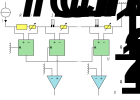
\includegraphics[scale=1]{../Figures_chap_exp/anderson_schema_reversed.pdf}
%\includegraphics[width=.2\textwidth]{../Figures_chap_exp/anderzoom.png}
\caption[Boucle d'Anderson]{Schéma électrique de la boucle d'Anderson. La boucle d'Anderson repose sur une boucle de jauges en série avec une résistance de référence, et deux étages d'amplification successifs. Le premier étage amplifie le signal brut des jauges (composante continue comprise) par un faible gain $\mathrm{G}_1$, et soustrait à chaque signal de jauge ainsi amplifié une tension de référence. Pour ce faire, une résistance de référence est ajoutée à la boucle, et la tension à ses bornes est amplifiée par le même gain que les jauges, mais sans soustraction. Le signal de référence amplifié est ensuite soustrait à tous les autres, dans chaque amplificateur de la boucle. Le deuxième étage est un amplificateur de grand gain $\mathrm{G}_2$. Des potentiomètres sont installés en série avec chaque jauge pour compenser les légères variations dans les valeurs de $R_r$ entre les jauges.}
\label{fig:anderson}
\end{figure}



\myparagraph{Principe}


La boucle d'Anderson\,\cite{anderson_nasas_1998} repose sur le principe de mettre en série à intensité $I$ constante plusieurs jauges $J_i$ de valeur au repos $R_r$, ainsi qu'une résistance de référence de valeur $R_r$ constante, et d'utiliser cette dernière pour éliminer la composante au repos des jauges. La tension $U_r$ aux bornes de la résistance de référence est soustraite aux tensions des jauges par un composant actif. La tension résultante est ensuite amplifiée par deux étages d'amplification successifs de gains $\mathrm{G}_1$ et $\mathrm{G}_2$, pour permettre l'acquisition du signal. Le schéma électrique de principe est détaillé en Figure\,\ref{fig:anderson}.



Si nous considérons une des jauges du circuit, et nommons $V_+$ et $V_-$ les potentiels à ses bornes, alors le signal en sortie du premier étage vaut

\begin{equation}
U_1=\mathrm{G}_1\times(V_+-V_-)-\mathrm{G}_1\times U_r
\end{equation}

En prenant en compte que $V_+-V_- = (R_r+\delta R)\times I$ et $U_r=R_r\times I$, nous obtenons

\begin{equation}
U_1=\mathrm{G}_1\times\delta R \times I
\end{equation}

Ainsi le premier étage élimine bien la composante au repos du signal des jauges.

Le signal en sortie du deuxième étage vaut

\begin{equation}
U_2=\mathrm{G}_2\times U_1=\mathrm{G}_1\times \mathrm{G}_2\times\delta R\times I
\end{equation}

Le signal de sortie s'exprime comme une fonction linéaire de $\delta R$, et donc de $\varepsilon_{\parallel}$.


La résistance de référence peut être physiquement déportée et positionnée proche de l'échantillon et des jauges de déformation. Elle a alors une résistance fixe mais est dans le même environnement électromagnétique que les autres jauges (longueur de câble, position, orientation, etc.). Ainsi si les jauges subissent un champ électromagnétique fort (bruit coloré, néons, signaux téléphoniques, etc.), la proximité de la référence permet d'annuler tout signal parasite par la soustraction effectuée dans le premier étage d'amplification. Afin de rendre les environnements électromagnétiques des jauges et de la référence plus proches encore, il est possible d'utiliser une jauge non solidaire du bloc pour remplir le rôle de référence.

La boucle d'Anderson dispose donc en théorie de nombreux avantages, en particulier sa linéarité exacte, sa relative simplicité de réglage, et sa capacité à résister au bruit. C'est pour cela que nous avons choisi de l'implémenter dans notre dispositif électronique. Cependant cette méthode fait intervenir une soustraction active et plusieurs étages d'amplification, pouvant générer du bruit.



\myparagraph{Mise en pratique -  évaluation du bruit}



\begin{figure}[htb]
\centering	
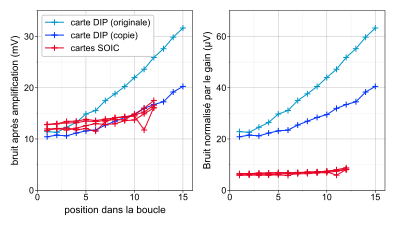
\includegraphics[scale=1]{../Figures_chap_exp/test_JPBox_fast.pdf}
\caption[Niveau de bruit dans nos dispositifs d'amplification]{Comparaison du niveau de bruit (écart type d'un signal à vide) entre les deux systèmes d'amplification. Les deux cartes du premier jeu, en bleu, génèrent un bruit croissant avec la distance de la jauge à la source de courant, témoignant d'une fuite de courant. Les 5 cartes du deuxième jeu, en rouge, bien qu'ayant un niveau de bruit brut à première vue similaire à celles du premier jeu, ont un niveau de bruit 4 fois moins grand une fois normalisé par le gain, et ce malgré une bande passante plus élevée. Leur fuite de courant est beaucoup plus faible, comme montré par la faible différence de niveau de bruit entre la première et la dernière jauge de la boucle.}
\label{fig:bruit}
\end{figure}




Lors de notre étude, nous avons fabriqué et utilisé deux jeux de circuits imprimés différents, implémentant chacun une boucle d'Anderson avec une approche différente, le deuxième ayant été dessiné et fabriqué pour combler les lacunes du premier. Les performances des deux systèmes sont comparées en Figure\,\ref{fig:bruit}.


\myparagraph{Premier jeu de cartes -- DIP}

Le premier jeu de cartes, utilisé dans cette étude jusqu'en janvier 2024, est adapté d'un circuit déjà existant, utilisé dans le groupe de J. Fineberg au \textit{Racah Institute of Physics} de la \textit{Hebrew University of Jerusalem}, conçu en 2012. Chaque carte consiste en une boucle de 15 jauges et d'une référence, avec deux étages d'amplification de gains $10\times50$. La bande passante de ce système est de \SI{500}{\kilo\hertz} (produit gain bande de $2.5\times10^8$). Nous avons utilisé en parallèle deux cartes de 15 voies, soit 30 jauges agencées en 10 rosettes, permettant 10 points de mesure simultanée à l'interface.

Ce jeu de cartes a plusieurs limitations intrinsèques à sa conception. Tout d'abord les amplificateurs utilisés sont des composants DIP (\textit{Dual Inline Package}), ce qui augmente l'espace physique occupé par les cartes, la quantité de chaleur dissipée par le système, et le niveau de bruit. De plus chaque amplificateur représente une fuite de courant, et ajoute du bruit dans le courant reçu par la jauge suivante. Le niveau de bruit augmente ainsi tout le long de la boucle jusqu'à masquer le signal. Cette dernière limitation est d'autant plus marquée que le circuit a initialement été développé pour des jauges de \SI{120}{\ohm}, et que nous l'utilisons avec des jauges de \SI{350}{\ohm}. Pour cette raison, la deuxième carte du jeu DIP est une copie légèrement remaniée de la première et son niveau de bruit en est réduit (Fig.\,\ref{fig:bruit}).


%%%%%%%%%%

En raison des limitations techniques de ce système, nous avons développé au long de notre étude un deuxième jeu de cartes, dont la conception a été finalisée en janvier 2024.


\myparagraph{Deuxième jeu de cartes -- SOIC}

Le deuxième jeu est composé de 5 boucles contenant chacune 12 jauges et une référence, ayant un gain de $10\times200$. La bande passante de ce système est de \SI{5}{\mega\hertz} (produit gain bande de $10^{10}$). Les 5 cartes sont insérées dans un unique boîtier blindé de format 2U.

Afin de combler les lacunes du système précédent, nous avons utilisé des composant SOIC (\textit{Small Outline Integrated Circuit}) plus récents et performants. Les circuits d'amplification sont équipés de nombreux filtres capacitifs et de ferrites limitant le bruit d'amplification et stabilisant l'alimentation, ainsi que de composants de haute impédance limitant les fuites de courant. Ces améliorations nous ont permis de réduire d'un facteur 3 à 8 l'écart type du bruit électronique normalisé par le gain par rapport au premier jeu de cartes (Fig.\,\ref{fig:bruit}).






\subsubsection{Reconstruction du tenseur des déformations 2D}



\begin{figure}[htb]
\centering	
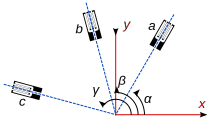
\includegraphics[scale=1]{../Figures_chap_exp/StrainRosetteAngles.pdf}
\caption[Reconstruction du tenseur des déformations]{Notations des angles dans une rosette à trois jauges de déformation. Les capteurs que nous utilisons sont des rosettes à trois jauges, écartées d'un angle de \ang{45} de part et d'autre de l'axe $y$, nommé axe principal de la rosette ($\alpha=\beta=\gamma=\ang{45}$). Dans notre étude, cet axe est disposé perpendiculairement à l'interface.}
\label{fig:anglerosette}
\end{figure}





Les jauges de déformation permettent des mesures de déformation uni-axiales, cependant nous cherchons à mesurer le tenseur des déformations complet à l'interface. Il est possible de reconstruire ce tenseur en utilisant 3 jauges de déformation disposées en rosette.

La géométrie du système permet de réduire le tenseur $[\varepsilon]$ à deux dimensions

\begin{equation}
{[\varepsilon]}
=
\begin{bmatrix}
	\varepsilon_{xx} & \varepsilon_{xy} \\
	\varepsilon_{xy} & \varepsilon_{yy}
\end{bmatrix}
\end{equation}
 

Pour calculer les composantes $\varepsilon_{xx}$, $\varepsilon_{xy}$ et $\varepsilon_{yy}$ du tenseur des déformations à partir de trois mesures non-coaxiales des déformations du bloc $\varepsilon_{\{a,b,c\}}$ (Fig.\,\ref{fig:anglerosette}) nous utilisons l'expression suivante :


\begin{align}[left=\empheqlbrace]
\begin{split}
		\varepsilon_a
	&=
		\dfrac{\varepsilon_{xx}+\varepsilon_{yy}}{2}+\dfrac{\varepsilon_{xx}-\varepsilon_{yy}}{2} \cos( 2 \alpha)+\varepsilon_{xy} \sin (2 \alpha)
	\\
		\varepsilon_b
	&=
		\dfrac{\varepsilon_x+\varepsilon_y}{2}+\dfrac{\varepsilon_x-\varepsilon_y}{2} \cos (2(\alpha+\beta))+\varepsilon_{x y} \sin (2(\alpha+\beta))
	\\
		\varepsilon_c
	&=
		\dfrac{\varepsilon_x+\varepsilon_y}{2}+\dfrac{\varepsilon_x-\varepsilon_y}{2} \cos (2(\alpha+\beta+\gamma))+\varepsilon_{x y} \sin (2(\alpha+\beta+\gamma))
\end{split}
\end{align}

Ainsi dans le cas d'une rosette de trois jauges écartées de \ang{45}, et dont l'axe de la jauge centrale est l'axe $y$, il vient

\begin{align}[left=\empheqlbrace]
\label{eq:rotation}
\begin{split}
		\varepsilon_{xx}
	&=
		\varepsilon_{a}-\varepsilon_{b}+\varepsilon_{c}
	\\
		\varepsilon_{yy}
	&=
		\varepsilon_{b}
	\\
		\varepsilon_{xy}
	&=
		\left(\varepsilon_{a}-\varepsilon_{c}\right)/2
\end{split}
\end{align}




\subsubsection{Disposition des jauges sur les blocs}


Le choix que nous avons effectué pour la plupart des expériences présentées est de disposer d'un côté du bloc une rosette tous les centimètres tout le long de l'interface, soit 15 rosettes, et 5 rosettes sur l'autre face, servant à contrôler la symétrie des contraintes appliquées. Les jauges d'intérêt ont ensuite été choisies en fonction des besoins de chaque expérience et des capacités du dispositif d'amplification utilisé. Les rosettes sont disposées à \SI{2 +- 0.2}{\milli\meter} de l'interface, permettant d'avoir un signal important au passage d'une rupture.
%tout en restant hors de la zone de régularisation des contraintes
Leur axe principal (Fig.\,\ref{fig:anglerosette}) est disposé perpendiculairement à l'axe de l'interface.


\subsection{Acquisition}


\subsubsection{Spécifications des acquisitions}

Le système d'acquisition dispose de 64 voies, dont 60 correspondent aux 60 jauges (20 rosettes) conditionnées par le système d'amplification, connectées par un connecteur blindé dédié. Les 4 autres voies sont accessibles par un connecteur coaxial standard, et peuvent servir à mesurer diverses observables. Dans notre étude, 2 de ces voies sont dédiées aux capteurs de forces normale et cisaillante, et une à un déclenchement accélérométrique, détaillé plus bas. Une voie est laissée libre pour de futures applications.

Un évènement de rupture typique durant de l'ordre d'une milliseconde (Sec.\,\ref{sec:LEFM}), les canaux sont acquis par salves de \SI{10}{\milli\second} à une fréquence d'acquisition de \SI{4}{\mega\hertz}, déclenchées par un accéléromètre. Cette acquisition rapide est doublée d'une acquisition lente, à \SI{315}{\hertz}, en continu sur une expérience. Les signaux acquis sont numérisés sur 14 bits avec un suréchantillonnage à \SI{40}{\mega\hertz}, sur une plage de tension d'entrée de [-4, 4] V, donnant une résolution de $10^{-5}\,\text{V}$.


\subsubsection{Déclenchement par accéléromètre}
\label{sec:accel}

Afin de détecter les évènements de glissement rapide de l'interface, et de donner un signal de déclenchement aux acquisitions rapides, nous utilisons un accéléromètre collé sur le bord d'un des blocs. L'accéléromètre agit comme un sismomètre et reçoit les ondes émises au moment d'un évènement de glissement. Son signal est généré par effet piézoélectrique, passif, et est d'une très faible puissance. Il doit donc être amplifié, puis converti en signal de logique transistor (TTL).

Le circuit d'amplification (Fig.\,\ref{fig:accel}) est composé d'un système d'amplification de grand gain réglable (jusqu'à 500). La sortie de l'amplificateur est connectée à l'entrée de deux multivibrateurs monostables en série. Un multivibrateur monostable est un composant électronique qui émet une impulsion TTL de longueur définie lorsque son entrée dépasse un seuil fixé. Ainsi un évènement de glissement va entraîner un déclenchement des deux multivibrateurs, et l'émission de deux impulsions TTL, une courte (quelques microsecondes) et une longue (quelques millisecondes), utilisées respectivement comme déclencheur de l'acquisition rapide et comme repère d'évènement de glissement dans l'acquisition lente.






\subsection{Traitement numérique des données acquises}
\label{sec:electroniquedonnées}

Les données brutes fournies par le boîtier d'acquisition sont converties en valeurs de tension, enregistrées en nombres flottants sur 64 bits, sous le langage de programmation Python3 (\texttt{<class 'numpy.float64'>}), permettant une précision de l'ordre de 16 chiffres significatifs. Le même langage est utilisé pour tous les traitements ultérieurs. Les données d'acquisition électronique sont rassemblées avec les données optiques (Sec.\,\ref{sec:optiquesdonnées}), et les traitements finaux et figures sont réalisés sous Python3\,\cite{van_rossum_python_2009, harris_array_2020,hunter_matplotlib_2007}.

Afin d'éliminer l'erreur systématique induite par le réglage des potentiomètres des jauges sur la valeur de tension mesurée, une valeur de référence prise avec les capteurs à vide lui est soustraite. La disposition des jauges est contrôlée en passant chaque bloc dans un scanner de documents à haute résolution. Ainsi la distance à l'interface des rosettes est vérifiée, et  la rotation de chacune peut si besoin être prise en compte et corrigée lors de la reconstruction du tenseur des déformations (Éq.\,\ref{eq:rotation}).

Nous avons également implémenté des méthodes numériques de réduction de bruit telles que des filtres, utilisées dans divers traitements de données et pour certaines représentations graphiques. Nous avons principalement utilisé des filtres passe-bas sous la forme de moyennes glissantes, mais aussi plus anecdotiquement des filtres passe-bande et coupe-bande, pour caractériser et éliminer des bruits colorés.


\newpage



\begin{figure}[h!]
\centering	
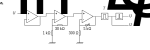
\includegraphics[scale=1]{../Figures_chap_exp/trigger.pdf}\\
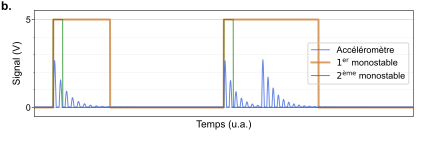
\includegraphics[scale=1]{../Figures_chap_exp/signal_accelero.pdf}
\caption[Système de déclenchement accélérométrique]{\textbf{a.}\,Schéma électrique du conditionnement de l'accéléromètre. Le circuit d'amplification se décompose successivement en un suiveur de grande impédance, un amplificateur de gain fixe, un amplificateur réglable, un multivibrateur monostable re-déclenchable à longue pulsation, puis enfin un multivibrateur monostable non re-déclenchable à pulsation courte. Cette combinaison permet de détecter les évènements de glissement, en passant outre les oscillations macroscopiques du système.  \textbf{b.}\,Représentation simplifiée de signaux réels. En bleu, un signal typique correspondant à l'accéléromètre amplifié. En ocre, la sortie du premier multivibrateur. En vert, la sortie du deuxième.}
\label{fig:accel}
\end{figure}



\vspace{10mm}

\section{Mesures Optiques}
\label{sec:optique}

En parallèle de l'acquisition électronique, nous imageons la surface des blocs à l'aide d'une caméra rapide. Cela nous permet un suivi optique autour de l'interface, et la mesure des déplacements des grains par corrélation d'images, à une précision de l'ordre de \SI{5}{\micro\meter}. Cette section détaille l'optique utilisée et les méthodes numériques implémentées pour l'analyse des images.

\subsection{Optique utilisée}

L'acquisition optique est réalisée à l'aide d'une caméra rapide Phantom V2511 pouvant aller de 100\,fps à 1\,Mfps. La caméra est équipée selon les besoins d'objectifs dont la focale varie de 85 à \SI{135}{\milli\meter}. La résolution maximale du capteur est de $1280\times800$ pixels, mais il est possible de n'utiliser qu'une portion du capteur, ce qui permet d'augmenter la vitesse d'acquisition. Nous avons principalement utilisé le capteur dans toute sa largeur pour filmer tout le long de l'interface à 100 ou 1\,000\,fps, mais des tests préliminaires ont été effectués jusqu'à 500 kfps.

L'acquisition peut être déclenchée par le même accéléromètre que celui utilisé pour le dispositif d'acquisition électronique.


\newpage

\subsection{Suivi des grains - recherche de motif}
\label{sec:suividesgrains}

La recherche de motif dans une image (\textit{template matching}) permet de trouver la position la plus probable d'un motif de référence donné dans une image le contenant. Un exemple emblématique de recherche de motif est la reconnaissance de texte, dans lequel les caractères d'écriture servent de motif de référence à chercher. Nous l'avons pour notre part utilisé pour détecter et suivre la position des cylindres à l'interface.




\subsubsection{Détermination des motifs à suivre par transformée de Hough}
\label{sec:paint}



\begin{figure}[htb]
\centering	

\includegraphics[scale=1]{../Figures_chap_exp/fullygran_zoom.pdf}
\caption[Interface entièrement granulaire]{Photographie de l'interface entièrement granulaire. Les cylindres sont déposés à l'interface et font face à la caméra. Leur face plane est blanche avec deux points noirs.}
\label{fig:facegrains}
\end{figure}



\begin{figure}[htb]
\centering	
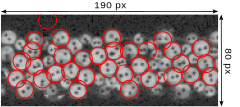
\includegraphics[scale=1]{../Figures_chap_exp/correlation_grains_0.pdf}
\caption[Détection des grains par transformée de Hough]{Détection initiale de la position des cylindres. Cette détection, effectuée par transformée de Hough, est corrigée manuellement pour éliminer les faux positifs et rajouter les cylindres non détectés.}
\label{fig:hough}
\end{figure}



Les cylindres sont disposés de telle sorte à ce que leur face circulaire soit contenue dans le plan filmé par la caméra, pour permettre de suivre leur mouvement en deux dimensions. Afin d'améliorer le contraste des images et la reconnaissance des faces, nous les avons peintes en blanc, et dessiné deux points noirs pouvant également servir à suivre leur rotation (Fig.\,\ref{fig:facegrains}). Les cylindres solidaires des blocs solides sont également peints pour être suivis. Dans le cas de l'interface à œil granulaire, afin de suivre le déplacement des blocs au niveau des parties solides de l'interface, le motif des cylindres a été reproduit en plusieurs points de la surface des blocs.


La recherche de cercles dans une image, et donc des faces des cylindres, est réalisée à l'aide d'une transformée de Hough (HCT)\,\cite{illingworth_survey_1988}. Ainsi, la position initiale de chaque cylindre est déterminée en appliquant une transformée de Hough à la première image de l'acquisition (Fig.\,\ref{fig:hough}). En raison des faux positifs et de la sensibilité aux variations de luminosité, la reproduction de cette détection sur toutes les images ne constitue pas une bonne méthode de suivi des cylindres. Nous utilisons pour cela une méthode de recherche de motif par corrélation.



\subsubsection{Recherche de motif par corrélation d'images numériques}

Nous notons la moyenne et l'écart type d'un signal $f$ comme $\mean{f}$ et $\sigma(f)$. L'élément d'indice $i$ d'un signal ou d'un vecteur $f$ (le pixel d'indice $i$ d'une image $f$) est noté $f_i$. Nous notons également dans cette section $\mathcal{F}$ l'opérateur Transformée de Fourier, et en gras et majuscule les transformées de Fourier de signaux, comme suit : $\mathbf{F} = \mathcal{F}(f)$. Nous noterons de plus pour toute matrice $A$ son complexe conjugué comme $A^*$, et pour toute autre matrice $B$ compatible, le produit de Hadamar entre les deux (terme à terme) comme $A\circ B$.


Le principe de la recherche de motif par corrélation est de comparer un motif donné à chaque sous-section de même taille de l'image dans laquelle il est recherché. Pour simplifier la description de ce principe, nous nous limitons dans cette section à la recherche d'un motif $g$ unidimensionnel de taille $m$ dans une image $f$ unidimensionnelle de taille $N$. Afin de simplifier la description mathématique du processus décrit (pour ne pas expliciter la prise en compte des bords de l'image), nous considérerons également des images toriques, c'est à dire que pour tout entier $k$ nous définissons $f_{N+k}:=f_{k}$ et $g_{m+k}:=g_{k}$.

L'outil utilisé pour réaliser cette comparaison est la corrélation croisée (ou covariance croisée) des deux images. En une dimension, pour une image initiale $f$ et un motif $g$, de valeurs moyennes $\mean{f}$ et $\mean{g}$, et d'écarts types $\sigma(f)$ et $\sigma(g)$, cette corrélation peut être exprimée comme un vecteur $r$ de taille $N$, tel que $r=[r_n]_{n\in\llbracket 1,N\rrbracket}$, avec

\begin{equation}
r_n=\dfrac{1}{\sigma(f)\times\sigma(g)}\times \sum\limits_{i=1}^m\left[
			( f_{n+i}-\mean{f} )
				\times
			( g_i-\mean{g} )\right]
\end{equation}

Cette opération peut être décrite dans l'espace de Fourier comme

\begin{equation}
\mathcal{F}(r) = \mathbf{R} = \mathbf{F}\circ\mathbf{G}^*
\end{equation}

Nous pouvons alors retrouver le vecteur de la position la plus probable du motif $\vec{\Delta}=\left[\Delta_x\right]$ en cherchant le maximum du vecteur de corrélation $r$, soit $\Delta_x = \arg\max\limits_i\{r_i\}$


Cette description se généralise en deux dimensions. Le vecteur de corrélation $r$ est alors une image de corrélation, de la même taille que $f$. La position du motif $g$ dans l'image, $\vec{\Delta}=[\Delta_x,\Delta_y]$, est alors exprimée comme

\begin{equation}
\vec{\Delta} = [\Delta_x,\Delta_y]
	   = \arg\max\limits_{(i,\,j)}\{r_{ij}\}
	   = \arg\max\limits_{(i,\,j)}\left\{
		   \mathcal{F}^{-1}
			   \left(
				   \mathbf{F}\circ\mathbf{G}^*
			   \right)_{ij}
		\right\}
\end{equation}


Nous obtenons ainsi la position la plus probable d'un motif dans une image. Cette position a une résolution au pixel.

L'implémentation algorithmique du cas général de cette méthode a une complexité asymptotique de $\mathcal{O}\left((m\times n) \times \allowbreak(M\times N)\right)$, où $m\times n$ et $M\times N$ sont les dimensions du motif et de l'image dans laquelle in est recherché. Dans le cas où les motifs se déplacent de quelques pixels ou moins entre chaque image, il est possible de restreindre le calcul de corrélation autour de la position connue du cylindre, donnant une complexité en $\mathcal{O}((m\times n)^2)$, par motif et par image.



\subsubsection{Application au suivi des grains}







La détection de cercles par transformée de Hough utilisée dans la première image permet d'en extraire, pour chaque cylindre, une sous-image carrée le contenant, qui constitue un motif de référence. Chaque motif ainsi obtenu est corrélé avec chaque image de la vidéo, donnant une série d'images de corrélation. La position du maximum dans ces images de corrélation donne la position des cylindres, permettant un suivi de leur position avec une résolution au pixel (Fig.\,\ref{fig:correl}). En pratique du fait du faible déplacement des cylindres entre deux images, les motifs ne sont corrélés à chaque itération du suivi qu'avec une fraction de chaque image, centrée autour de la position du cylindre à l'itération précédente. Les positions ainsi mesurées sont quantifiées à l'échelle d'un pixel, qui dans les conditions expérimentales que nous avons choisies (mesure de toute la longueur de l'interface, soit \SI{150}{\milli\meter}, avec un capteur large de 1280 pixels) correspond à \SI{120}{\micro\meter}. Cette quantification s'accompagne d'oscillations rapides lorsque le centre du grain observé est entre deux pixels (Fig.\,\ref{fig:trackingres}a). Il est cependant possible d'améliorer cette résolution.






\begin{figure}[p]
\centering	
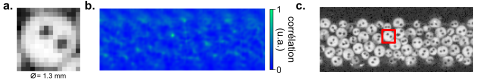
\includegraphics[scale=1]{../Figures_chap_exp/correlation_grains_1.pdf}
\caption[Détection des grains par PTV]{\textbf{a.}\,Motif extrait de la première image d'une acquisition. \textbf{b.}\,Image de corrélation du motif de gauche avec la dernière image de l'acquisition. \textbf{c.}\,Position détectée du motif de gauche dans la dernière image de l'acquisition. La position détectée correspond au maximum de corrélation, représenté par la tâche blanche la plus claire, au centre de l'image de corrélation.}
\label{fig:correl}
\end{figure}



\begin{figure}[p]
\centering	
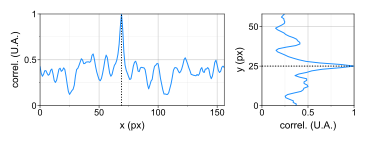
\includegraphics[scale=1]{../Figures_chap_exp/correlation_grains_2.pdf}
\caption[Profil de corrélation]{Coupes transversales horizontale et verticale de la matrice de corrélation de la Figure\,\ref{fig:correl}, centrées sur le maximum de corrélation. Les deux coupes montrent que le maximum est situé au sommet d'un halo, qui peut être ajusté par une fonction gaussienne.}
\label{fig:gausscor}
\end{figure}


\begin{figure}[p]
\centering	
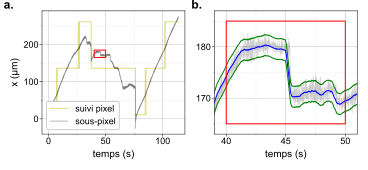
\includegraphics[scale=1]{../Figures_chap_exp/tracking_grains.pdf}
\caption[Suivi du mouvement d'un grain]{\textbf{a.}\,Suivi du mouvement d'un cylindre au cours d'une expérience. Un millimètre est balayé par 8 pixels. Nous observons la discrétisation et les oscillations rapides de la position au pixel (ligne jaune), et la position sous-pixel (ligne grise). L'intérieur du rectangle rouge est reproduit à droite. \textbf{b.}\,Détail du suivi du même cylindre. La courbe grise représente le suivi sous-pixel, et la courbe bleue représente la moyenne glissante sur 40 images de la position mesurée. La largeur du bruit associé au suivi, de l'ordre de \SI{2}{\micro\meter}, est déterminée par l'écart type médian des positions des cylindres lorsqu'ils sont immobiles, et est représentée par les deux courbes vertes.}
\label{fig:trackingres}
\end{figure}







\subsubsection{Amélioration de la résolution par PTV}



Afin d'améliorer la résolution du suivi des cylindres et de la placer en dessous de l'échelle du pixel, nous avons implémenté une méthode de \textit{Particle Tracking Velocimetry} (PTV). Il s'agit d'une interprétation lagrangienne de la \textit{Particle Image Velocimetry} (PIV)\,\cite{raffel_particle_2007}, reposant sur les mêmes principes généraux.

Cette méthode consiste en l'ajustement du pic de corrélation par une fonction gaussienne, au moyen d'un estimateur à trois points\,\cite{raffel_particle_2007}. En effet dans nos images, en raison de la largeur et de la forme circulaire des faces des cylindres, le maximum de corrélation est au centre d'un halo de hautes corrélations suffisamment symétrique pour être considéré Gaussien à l'ordre\,2 en son sommet (Fig.\,\ref{fig:gausscor}). Cet ajustement est effectué sur la matrice de corrélation normalisée et tronquée aux 4 points adjacents à sa valeur maximale. Ainsi si nous notons $\vec{\Delta} = \left[\Delta_x,\Delta_y\right]$ la position du maximum de la matrice de corrélation $r$, et donc la position du motif au pixel, nous pouvons définir $\vec{\delta}=\left[\delta_x,\delta_y\right]$ l'écart sous-pixel donné par l'ajustement :

\begin{align}[left=\empheqlbrace]
\begin{split}
\delta x &=\frac{1}{2}\times \dfrac{\ln(r_{i-1,j})-\ln(r_{i+1,j})}{\ln(r_{i-1,j})-2\times\ln(r_{i,j})+\ln(r_{i+1,j})}\\
\delta y &=\frac{1}{2}\times \dfrac{\ln(r_{i,j-1})-\ln(r_{i,j+1})}{\ln(r_{i,j-1})-2\times\ln(r_{i,j})+\ln(r_{i,j+1})}
\end{split}
\end{align}

La valeur de la position sous-pixel du centre du halo, et donc du motif, est alors $\vec{D} = \vec{\Delta}+\vec{\delta}$.

\subsubsection{Évaluation de la résolution par PTV}



\begin{figure}[hbt]
\centering
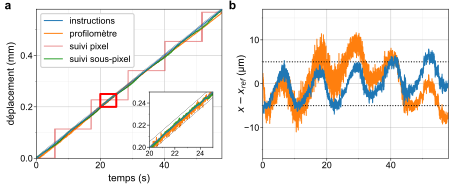
\includegraphics[scale=1]{../Figures_chap_exp/figure_S2_res_only.pdf}
\caption[Évaluation de la résolution de la PTV]{Évaluation de la résolution du suivi sous-pixel. \textbf{a.}\,Le déplacement commandé $x_{com}$ est une rampe de position à vitesse fixée (courbe bleue), mesurée par un profilomètre confocal $x_{prof}$ (orange). La mesure pixel (rose) est discrétisée, et la mesure  sous-pixel $x_{opt}$ (verte) est comprise dans une gaine de \SI{+-5}{\micro\meter} autour de la valeur de commande. \textbf{b.}\,Écart entre la position mesurée par le suivi sous-pixel $x_{opt}$ et la position de commande $x_{com}$ (bleu), ainsi qu'entre $x_{opt}$ et $x_{prof}$ (orange). La périodicité observée correspond aux changements de valeur du suivi au pixel.}
\label{fig:trackingres2}
\end{figure}


Afin d'évaluer la précision de cette méthode nous l'avons testée sur des grains en déplacement contrôlé. Nous avons créé plusieurs scripts de déplacement permettant de contrôler
%\href{https://youtu.be/???}{\textcolor{black}{informatiquement}}
informatiquement
la position de la platine motorisée et donc des blocs et cylindres qui en sont solidaires. Pour déterminer la résolution de la méthode de suivi, une translation à vitesse constante de \SI{10}{\micro\meter\per\second} est imposée au bloc inférieur, sans chargement normal. Afin de s'assurer de la bonne exécution des commandes par la platine, nous mesurons sa position à l'aide d'un profilomètre confocal commercial, d'une résolution de l'ordre d'un micromètre. Nous comparons ensuite la valeur de commande $x_{com}(t)$, la mesure du profilomètre $x_{prof}(t)$, et la mesure du suivi des grains solidaires du bloc en translation $x_{opt}(t)$ (Fig.\,\ref{fig:trackingres2}a). Les trois courbes suivent la même tendance, et la déviation standard de $x_{com}(t)-x_{opt}(t)$ vaut \SI{1.5}{\micro\meter}. Nous quantifions la précision du suivi à l'aide de la règle des 3 sigmas (incluant 99.7\% des valeurs), ce qui donne une limite de résolution de \SI{5}{\micro\meter}.

Une observation plus fine de l'écart entre la commande et le suivi optique révèle que $x_{com}(t)-x_{opt}(t)$ oscille de manière périodique (Fig.\,\ref{fig:trackingres2}b, courbe bleue). Cette même oscillation apparaît également lorsque l'on calcule $x_{com}-x_{prof}$ (courbe orange), et ne peut donc pas être imputée au mouvement de la platine, mais bien au suivi des cylindres. La limite de résolution déterminée précédemment de l'ordre de \SI{5}{\micro\meter} n'est donc en réalité pas due à une erreur aléatoire mais à un biais périodique. Les oscillations correspondent aux changements de valeur du suivi au pixel, et représentent un défaut majeur de notre méthode de suivi. Elles sont le facteur limitant dans les mesures de déplacements supérieurs ou de l'ordre d'un pixel, soit \SI{120}{\micro\meter}. En revanche, lorsque le déplacement mesuré est beaucoup plus faible que la taille d'un pixel, l'amplitude du bruit associé à la mesure optique est de l'ordre d'un micromètre.


\subsection{Traitement des données de suivi optique}


Les données brutes nous renseignent sur les mouvements absolus des cylindres au cours du temps. Nous effectuons plusieurs traitements sur celles-ci afin d'en faciliter l'analyse.

Le repère utilisé dans cette section est celui de l'interface, c'est à dire que l'axe horizontal $\vec{e_x}$ coïncide avec l'interface, et l'axe vertical $\vec{e_y}$ lui est perpendiculaire, orienté vers le haut. Les cylindres sont indexés par un entier $i$, et leurs positions sont notées $\vec{X}_i = (x_i,\,y_i)$.



\subsubsection{Classement des grains}
\label{sec:classement}



Afin de raffiner l'analyse des mouvements des cylindres, ceux-ci doivent être catégorisés en fonction de leur position sur le bloc relativement à l'axe de l'interface. Les différentes catégories sont les suivantes :

\begin{itemize}
\bitem $\{boundary\}$ et $\{bulk\}$ : Les cylindres solidaires d'un bloc solide sont catégorisés dans $\{boundary\}$, tandis que les cylindres libres sont dans la catégorie $\{bulk\}$. Chaque cylindre se voit attribuer manuellement une des deux catégories au moment de leur détection initiale. Les cylindres de la catégorie $\{boundary\}$, en les considérant bien répartis de part et d'autre de l'interface, permettent de définir $\bar{y} = \left\langle y_i\right\rangle_{i\in\{boundary\}}$ la hauteur approximative de la ligne d'interface, et $\bar{x}= \left\langle x_i\right\rangle_{i\in\{boundary\}}$ la position horizontale du centre des blocs.
\end{itemize}

Les catégories suivantes ne sont définies que pour les cylindres catégorisés dans $\{boundary\}$.

\begin{itemize}
\bitem $\{top\}$ et $\{bottom\}$ : les cylindres tels que $y_i>\bar{y}$ sont dans $\{top\}$, les autres $\{bottom\}$.

\bitem $\{left\}$, $\{middle\}$ et $\{right\}$ : Ces catégories ne sont pertinentes que dans le cas de l'interface avec œil granulaire. Les cylindres tels que $\abs{x_i-\bar{x}}<\ell_{eye}/2$ (appartenant à l'œil granulaire) sont catégorisés dans $\{middle\}$. Parmi les autres, ceux tels que $x_i<\bar{x}$ sont dans $\{left\}$, et tels que $x_i>\bar{x}$ dans $\{right\}$. Nous définissons également $\{solid\}=\{left\}\cup\{right\}$ et $\{eye\}=\{middle\}$.

\bitem Classification par paires : Les cylindres de $\{boundary\}$ étant généralement disposés de manière symétrique de part et d'autre de l'interface, il est possible de les classer par paire à partir de leur position initiale, soit manuellement, soit automatiquement. Pour qu'une paire de cylindres $(i,j)$ soit valide, il faut tout d'abord que l'un soit dans $\{top\}$ (sans perte de généralité $i$), l'autre dans $\{bottom\}$, et tous les deux dans la même portion d'interface dans le cas du système à œil granulaire. Le critère d'appariement est alors
\nopagebreak[4]
\begin{align}[left=\empheqlbrace]
\begin{split}
\forall m  \in\{bottom\},&\quad\abs{x_i-x_j}<\abs{x_i-x_m}\\
\forall n  \in\{top\},&\quad\abs{x_i-x_j}<\abs{x_n-x_j}
\end{split}
\end{align}

\end{itemize}

%Dans les définitions des sections suivantes, nous considèrerons uniquement les grains de la catégorie $\{boundary\}$, c'est à dire les grains solidaires des blocs solides.




\subsubsection{Correction du suivi des grains}
\label{sec:rotat}

\begin{figure}[htb]
\centering
\includegraphics[scale=1]{../Figures_chap_exp/figure_5_rotat.pdf}
\caption[Correction de la rotation de l'interface]{Effet de la rotation de l'interface relativement à la caméra sur le déplacement mesuré des grains. Cet effet est corrigé en temps réel par un ajustement de la position de l'interface.}
\label{fig:rotat}
\end{figure}

La mesure de l'évolution de la position d'un cylindre et du glissement interfacial peuvent être perturbées par des mouvements parasites. Les principaux sont la rotation et la translation des blocs dans leur ensemble lors de leur cisaillement dues à la flexibilité du cadre de la presse, et les déformations élastiques des blocs.


\myparagraph{Influence de la rotation de l'interface}

La rotation et le déplacement de l'axe de l'interface augmentent avec la force cisaillante appliquée au système. Leur amplitude peut atteindre 1 mm et \ang{0.2}, ce qui peut mener à détecter à tort un glissement relatif entre deux cylindres de part et d'autre de l'interface (Fig.\,\ref{fig:rotat}). De plus le réglage de l'horizontalité de la caméra a une précision de seulement \ang{0.1}. Il n'est donc pas raisonnable de considérer que les axes de la caméra coïncident à tout moment avec l'axe naturel de l'interface.

Afin d'éliminer les déplacements parasites, nous projetons les coordonnés mesurées dans le référentiel de la caméra sur le référentiel naturel de l'interface. Pour ce faire, nous mesurons la position et la rotation de l'interface par rapport à l'axe horizontal de la caméra $\vec{e}_{x,cam}$. La classification des cylindres dans les catégories $\{top\}$ et $\{bottom\}$ permet de définir deux ajustements linéaires respectivement de la position des cylindres solidaires du bloc supérieur $y_{top}(t)=a_{top}(t)\times x_{cam}+b_{sup}(t)$, et du bloc inférieur $y_{bot}(t)=a_{bot}(t)\times x_{cam}+b_{bot} (t)$. Ces deux ajustements permettent à leur tour de définir l'équation de la position $y_{int}$ de l'interface dans le référentiel de la caméra $y_{int} = (y_{bot}+y_{top}) = a(t) \times x_{cam} + b(t)$. Pour un point de coordonnées $(x_0,y_0)$ dans le référentiel de la caméra, ses nouvelles coordonnées $(x_1,y_1)$ dans le référentiel de l'interface sont


\begin{align}[left=\empheqlbrace]
\begin{split}
x_1&= \dfrac{x_0+ay_0-a b}{\sqrt{a^2+1}} \\
y_1&= \dfrac{y_0-a x_0-b}{\sqrt{a^2+1}}
\end{split}
\end{align}

Cette projection dans le référentiel naturel de l'interface est effectuée lors du traitement des données issues du suivi des cylindres, et précède tous les autres traitements et calculs appliqués au cours de l'analyse.

\myparagraph{Influence de la différence de hauteur des cylindres}


\begin{figure}[htb]
\centering
\includegraphics[scale=1]{../Figures_chap_exp/figure_S1.pdf}
\caption[Effet de la déformation des blocs]{Effet de la déformation des blocs sur le déplacement mesuré des grains. Cet effet est négligeable dans le cadre de notre étude.}
\label{fig:defor}
\end{figure}

La différence de hauteur $h$ entre les paires de faces de cylindres de l'œil granulaire et celles des portions solides est de l'ordre de \SI{4}{\milli\meter}, et peut introduire des erreurs dans la mesure des déplacements en raison de la déformation des blocs en cisaillement (Fig.\,\ref{fig:defor}). Évaluons l'amplitude de cet effet dans le cas le plus défavorable. Nous considérons que la force de cisaillement atteint $F_S=\SI{1500}{\newton}$, avec $A=150\times\SI{10}{\milli\meter\squared}$ l'aire de contact entre les deux blocs, alors $\sigma_{xy}=F_S/A=10^6\,\text{Pa}$. Le déplacement $\delta x$ entre deux faces d'une même paire, à distance $h$, est alors

\begin{equation}
\delta x = \frac{2h\sigma_{xy}}{E/(2(1+\nu))}
\end{equation}

Ainsi nous trouvons $\delta x_g=\SI{9}{\micro\meter}$ et $\delta x_s=\SI{5}{\micro\meter}$. L'écart entre les deux quantités est inférieur à la résolution obtenue par le suivi PTV, et l'effet réel peut donc être négligé.






\subsubsection{Format des données}
\label{sec:optiquesdonnées}

Les données brutes acquises par la caméra sont des images en nuances de gris sur 12 bits, cependant le format utilisé pour le traitement des images est limité à 8 bits. Les images sont sauvegardées sans compression ni traitement sous le format \texttt{tiff}. Les mesures détaillées dans cette section et la suivante sont effectuées sous MatLab\,\cite{matlab_9501067069_2018}, et les données sont sauvegardées sous le type \texttt{double}, permettant une précision de l'ordre de 16 chiffres significatifs. Les données ainsi obtenues sont manuellement traitées pour éliminer les erreurs potentielles (fausses détections, cylindres mal suivis, images corrompues). Une partie des données est exportée après traitements sous Python3, pour être analysée avec les données d'acquisition électronique (Sec.\,\ref{sec:electroniquedonnées}).







\subsection{Expérience simulée et conditions réelles}
\label{sec:obsoptique}


\begin{figure}[htb]
\includegraphics[scale=1]{../Figures_chap_exp/figure_S2_delta_only.pdf}
\caption[Définition de $\delta_{IE}$ et $S$]{Déplacement d'un seul des blocs commandé par un script. \textbf{a.}\,Mesure du déplacement interfacial $\delta_{tot}$. Les évènements détectés sont marqués par les lignes en pointillés noirs. \textbf{b.}\,Évolution du glissement inter-évènement $\delta_{IE}$. \textbf{c.}\,Évolution du glissement inter-évènement normalisé $S$.}
\label{fig:delta}
\end{figure}


Dans cette section nous présentons brièvement le comportement typique dit de \textit{stick-slip} que nous observons dans les expériences que nous avons menées, et détaillons les définitions des grandeurs d'intérêt que nous étudions, par le biais de l'exemple d'une expérience simulée.

\subsubsection{Mouvement de stick-slip et glissement inter-évènement}
Lors d'une expérience de cisaillement de deux blocs pressés, le mouvement relatif des blocs est saccadé. Dans un modèle idéal, ce mouvement est constitué d'une alternance de phases de \textit{stick} de durée $T$, durant lesquelles le déplacement relatif des blocs à l'interface est nul, et d'évènements rapides de \textit{slip}, où l'interface glisse d'une distance $d_0$. Cette succession de phases est périodique, de période $T$ dépendant des paramètres de chargement. Le déplacement relatif de l'interface $\delta_{tot}^{ideal}(t)$ est alors une fonction constante par morceaux

\begin{equation}
\delta_{tot}^{ideal}(t)= d_0\times\floor{\frac{t}{T}}
\end{equation}

Dans une expérience réelle de stick-slip, le mouvement comporte une alternance de longues phases de stick (de durée moyenne $\mean{T}$, de l'échelle de la seconde), durant lesquelles le déplacement relatif des blocs est quasi-nul (à l'échelle du micromètre), et des évènements courts de slip (à l'échelle de la centaine de milliseconde), qui concentrent la majeure partie du déplacement (à l'échelle du millimètre). Dans certaines configurations que nous étudions le glissement ayant lieu entre les phases de slip peut atteindre le même ordre de grandeur que celui ayant lieu pendant celles-ci. Nous vérifions à l'aide d'une expérience simulée que le suivi des grains que nous avons implémenté permet bien de mesurer le glissement entre les évènements de slip.


\subsubsection{Expérience simulée : stick-slip avec glissement inter-évènement}



Afin de simuler un mouvement de stick-slip comportant du déplacement lent entre les évènements de slip, nous contrôlons la position du bloc inférieur non-chargé, au moyen de la platine motorisée, pilotée par un script (Fig.\ref{fig:delta}a). Les cylindres solidaires du bloc sont suivis par imagerie. Les instructions données sont des cycles de 5 secondes sans mouvement, 5 secondes de déplacement uniforme à \SI{20}{\micro\meter\per\second} (glissement lent), et un saut brusque de \SI{100}{\micro\meter} (évènement de slip).


Cette expérience a pour but de vérifier que notre méthode de suivi et de traitement mesure bien \SI{100}{\micro\meter} de déplacement par phase de slip, et \SI{100}{\micro\meter} par phase inter-évènement. Pour ce faire nous mesurons le déplacement $\delta_{tot}$, détectons les instants $\{t_{k}\}_{k\in\mathbb{N}}$ des évènements de slip, et en déduisons le déplacement inter-évènement $\delta_{IE}$. Les mesures de ces quantités dans l’expérience simulée et leurs définitions dans les expériences réelles sont détaillées dans les trois sections suivantes.




\subsubsection{Glissement interfacial total}
\label{sec:totslip}

Pour l'expérience simulée, afin de déterminer le déplacement total des cylindres $\delta_{tot}$, nous effectuons la moyenne des déplacements de tous les grains. Nous vérifions bien que ce suivi est correct (Fig.\,\ref{fig:delta}a).


Dans le cas d'une expérience réelle, l'application d'une force entraîne un déplacement général de tous les grains dans le sens du cisaillement, $\delta_{tot}$ est alors défini comme déplacement \textit{relatif} des blocs à l'interface. Cette mesure est permise par le classement des grains selon leur appartenance à la catégorie $\{top\}$ ou $\{bottom\}$, donnant

\begin{equation}
\delta_{tot}(t) = \mean{x_i}_{i\in\{top\}}(t) - \mean{x_j}_{j\in\{bottom\}}(t)
\end{equation}


Pour d'autres usages, il est possible de raffiner cette quantité par portion d'interface ou par paire de grains. Par exemple le déplacement relatif des  cylindres dans la partie solide-solide de l'interface avec œil granulaire est noté $\delta_{tot}^{solid}(t)$, et est défini comme

\begin{equation}
\delta_{tot}^{solid}(t) = \mean{x_i}_{i\in\{top\}\cap\{solid\}}(t) - \mean{x_j}_{j\in\{bottom\}\cap\{solid\}}(t)
\end{equation}

Nous cherchons maintenant à distinguer le mouvement effectué durant les phases de slip du glissement lent effectué entre celles-ci.


\subsubsection{Détection des évènements de glissement rapides}
\label{sec:detecoptique}

Afin d'étudier indépendamment chaque phase du mouvement, il nous faut détecter les évènements de glissement rapide. Cette détection est effectuée par un filtrage passe-haut de $\delta_{tot}(t)$ mettant en évidence ses changements brusques. Nous obtenons ainsi une liste de temps $\{t_{k}\}_{k\in\mathbb{N}}$ correspondant à chaque évènement de glissement rapide (Fig.\,\ref{fig:delta}, lignes pointillées). Ces temps permettent également de synchroniser les mesures optiques avec les mesures électroniques, dans lesquelles les évènements sont repérés par un signal accélérométrique (Sec.\,\ref{sec:accel}).

Afin de définir les limites des phases de stick, il nous faut considérer une marge autour de chaque temps $t_k$ assurant qu'aucun mouvement d'une phase de slip ne soit comptabilisé dans une phase de stick. Nous notons $t_k^-$ et $t_k^+$ les temps limites de chaque évènement, $t_k^- = t_k-\tau^-$ correspondant à l'instant juste avant l'évènement de glissement, et $t_k^+ = t_k+\tau^+$ au temps à partir duquel l'interface est stabilisée. La valeur de $\tau^-=\SI{0.05}{\second}$ est choisie constante, tandis que la valeur de $\tau^+$ est définie en fonction du comportement de l'interface. Elle est prise de façon à s'assurer que la phase de glissement rapide soit bien terminée, et que les vibrations de la table optique supportant la presse, dues à l'évènement, soient atténuées. La durée de cette phase de vibrations dépend de la quantité d'énergie relâchée par l'évènement, elle-même proportionnelle à la période à laquelle les phases de slip se répètent. Ainsi nous définissons $\tau^+$ comme une fonction croissante de $\mean{T}$, variant de \SI{0.15}{\second} à \SI{0.5}{\second}. Dans l'expérience de stick-slip simulée, les évènements sont bien détectés (Fig.\ref{fig:delta}a, lignes pointillées).


\subsubsection{Glissement inter-évènement}

La détection des évènements de glissement rapide permet enfin de définir le glissement inter-évènement $\delta_{IE}(t)$. Il correspond au glissement interfacial entre les évènements de glissement rapide, cumulé tout au long de l'expérience, et est défini comme

\begin{equation}
\delta_{IE}(t) = \delta_{tot}(t)-\sum_{t_k\leq t}\Big(\: \delta_{tot}(t_k^+)-\delta_{tot}(t_k^-)\:\Big)
\end{equation}

Cette grandeur peut se calculer pour une catégorie des cylindres suivis, et est alors notée avec la catégorie en question en exposant, $\delta_{IE}^{eye}$ pour la catégorie $\{eye\}$ par exemple. Lorsque nous représentons $\delta_{IE}(t)$, nous indiquons uniquement ses valeurs aux différents $t_k^+$ (Fig.\,\ref{fig:delta}), c'est à dire

\begin{equation}
\delta_{IE}(t_k^+) = \delta_{tot}(t_k^+)-\sum_{\kappa\leq k} \Big(\:\delta_{tot}(t_\kappa^+)-\delta_{tot}(t_\kappa^-)\:\Big)
\end{equation}


Dans le cas de l'expérience simulée présentée, la valeur de $\delta_{IE}(t)$ imposée par le script augmente de \SI{100}{\micro\meter} entre chaque évènement. La valeur que nous mesurons en pratique montre bien cette augmentation (Fig.\,\ref{fig:delta}b), bien que la valeur mesurée soit 1 à 2\% plus faible, en raison de la marge $\tau^-+\tau^+$ prise autour de chaque $t_k$.

\pagebreak

L'extraction du glissement inter-évènement et sa représentation sous la forme de la suite de ses valeurs permettent de déterminer la proportion du déplacement total de l'interface se faisant entre les évènements de glissement rapide. Afin d'évaluer cette proportion, nous définissons le glissement inter-évènement normalisé $S(t)$ comme

\begin{equation}
S(t) = \dfrac{\delta_{IE}(t)}{\delta_{tot}(t)}
\end{equation}

De même que $\delta_{IE}$ nous représentons généralement cette quantité de manière discrète, à chaque $t_k^+$ (Fig.\,\ref{fig:delta}c). Cette mesure de la proportion de glissement effectuée entre les évènements de glissement rapide est sous-estimée en raison de la largeur de la marge $\tau^-+\tau^+$ prise autour de chaque $t_k$. Dans le cas de l'expérience simulée, nous trouvons $S\sim 0.49$, pour une valeur attendue de $S=0.5$, l'écart s’expliquant par cette largeur.




\section{Conclusion}

Au cours de ce chapitre nous avons présenté le dispositif expérimental que nous avons développé durant cette thèse. Ce dispositif nous permet de presser et cisailler des plaques minces de PMMA, de plusieurs géométries et pouvant encapsuler un milieu granulaire bidimensionnel, en ayant une mesure précise des forces que nous leur appliquons. Les plaques sont équipées d'une électronique de précision permettant l'acquisition simultanée du signal de 20 rosettes (60 jauges) à une fréquence de \SI{4}{\mega\hertz}, nous offrant la résolution et la rapidité nécessaires à la mesure du champ des déformations à l'interface qu'elles forment lors d'une expérience. Cette mesure est complétée par un suivi par imagerie de la position des grains à l'interface qui nous permet de caractériser en détail les déplacements de ceux-ci à l'échelle micrométrique. Nous avons également introduit des quantités d'intérêt pour l'étude de l'interface en œil granulaire présentée dans le Chapitre\,\ref{sec:chaparticle}, notamment les mesures de glissement interfacial durant et entre les évènements de glissement rapide.

Grâce à ce dispositif et à la précision de son instrumentation, nous étudions et présentons par la suite les interfaces granulaires, et notamment l'influence d'une hétérogénéité, sous la forme d'un œil granulaire, sur le comportement de celles-ci.







\chapter[Ruptures sismiques -- Glissement asismique]{Ruptures sismiques initiées par un glissement asismique}
\label{sec:chaparticle}
\vspace*{-0.5cm}


% Les failles sismiques sont composées de couches successives de roches, de cohésion et de granulométrie variables, mises en mouvement par cisaillement élastique. Elles arborent une physique riche et complexe, dont le comportement est difficilement prédictible, et les étudier est un enjeu scientifique majeur, tant pour leur compréhension que leur surveillance, et la prévention des séismes.

Les séismes, évènements rapides de rupture de l'interface, ne sont pas le seul moyen par lequel les failles relâchent l'énergie élastique qu'elles emmagasinent. Cette énergie peut également être libérée au travers d'évènements de glissement lent (Fig.\,\ref{fig:extract_review})\,\cite{peng_integrated_2010,burgmann_geophysics_2018}. Ces évènements lents ont tout d'abord été découverts dans les zones de subduction puis observés dans d'autres systèmes de failles, transformantes et en zones de décrochement (Fig.\,\ref{fig:typesdefailles}) avec l'amélioration des techniques de mesure\,\cite{harris_large_2017}. Ces séismes lents peuvent affecter de larges portions d'un système de failles, et relâcher des quantités d'énergie comparables à celles relâchées par les séismes rapides\,\cite{dragert_silent_2001}. Ils peuvent aussi être très localisés, et détectés indirectement par la déstabilisation de l'interface qui en résulte (phénomène nommé \textit{Episodic tremor and slip})\,\cite{chen_scaling_2009,shelly_non-volcanic_2007,tan_connecting_2020,rogers_episodic_2003}. Le rôle des zones de déplacement lent, dites \textit{asismiques} ou \textit{découplées}, sur la déstabilisation des zones en mouvement de stick-slip, dites \textit{sismiques} ou \textit{couplées}, reste pourtant méconnu\,\cite{radiguet_triggering_2016,dragert_silent_2001}.


\begin{figure}[h!]
\centering
\includegraphics[scale=1]{../Figures_chap_article/failles.pdf}
\caption[Types de failles]{Les trois grands types de failles. La faille normale (\textbf{a}) apparaît dans les systèmes en extension. La faille inverse (\textbf{b}) apparaît dans les systèmes en compression comme les zones de subduction. La faille transformante (\textbf{c}) apparaît dans les zones de coulissement entre des plaques tectoniques.}
\label{fig:typesdefailles}
\end{figure}


L'apparition de cette diversité de comportements, et la difficulté de leur étude, sont dues à la complexité des interfaces considérées. En effet celle-ci implique la prise en compte d'une multitude de paramètres, tels que la teneur en eau des roches, leur viscosité, leur nature, la géométrie des failles ou encore la présence d'une couche de gouge, une roche broyée non-cohésive, dans le système de failles. Les expériences en laboratoire telles que celles que nous avons menées nous donnent une opportunité unique d'analyser séparément l'influence de chacun de ces paramètres, en contrôlant les caractéristiques principales d'une interface frictionnelle, telles que sa composition, le chargement qui lui est appliqué, ou la présence d'hétérogénéités. Elles nous permettent également d'instrumenter densément le milieu, et de multiplier les expériences, et donc d'étudier l'influence de ces paramètres et de comprendre les mécanismes microscopiques responsables des phénomènes de grande échelle qui en émergent.

\pagebreak

Dans ce chapitre, nous étudions l'influence d'une hétérogénéité dans la composition de l'interface sur le comportement d'une faille sismique modèle. Cette interface prend dans notre étude la forme d'une interface frictionnelle solide-solide composée de deux plaques minces de polyméthacrylate de méthyle (PMMA) perturbée par l'inclusion d'un milieu granulaire dense sur une portion de sa longueur. La conclusion majeure des résultats présentés est qu'au sein d'une faille modèle, une hétérogénéité de composition à l'interface créé un patch en glissement lent entre les évènements sismiques. Ce patch s'étend au-delà de l'hétérogénéité et agit comme un précurseur de rupture, menant à la déstabilisation de l'interface frictionnelle par la propagation d'une rupture rapide. La longueur de ce patch est d'autant plus élevée que l'hétérogénéité est dense et chargée.

%Ce chapitre présente tout d'abord plus en détail le système d'interface en \textit{œil granulaire} étudié, et les observables que nous utiliserons pour décrire son comportement, puis présente nos observations expérimentales des modifications du cycle de stick-slip dues à l'inhomogénéité de composition, et présente enfin une discussion de ces résultats et les perspectives futures ouvertes par notre étude.


\begin{figure}[h!]
\centering
\includegraphics[scale=1]{../Figures_chap_article/extract_review.pdf}
\caption[Faille en glissement lent]{Structure et comportement d'une faille sismique subissant du glissement lent (extrait de\,\cite{burgmann_geophysics_2018}). \textbf{a.}\,Illustration schématique de la distribution du glissement sismique et asismique dans une portion de la faille transformante de San Andreas partiellement couplée. \textbf{b.}\,Distribution du glissement sismique et asismique sur une zone de subduction partiellement couplée.}
\label{fig:extract_review}
\end{figure}





\newpage

\minitoc


\newpage








\section{Système étudié -- définitions}

Cette section décrit l'interface en \textit{œil granulaire}, et le dispositif expérimental utilisé au cours des expériences analysées dans ce chapitre. Ce dispositif est détaillé dans le Chapitre\,\ref{sec:chapxp}. Nous introduisons également notre paramètre de contrôle, le \textit{contraste de chargement} $C_\sigma$ caractérisant la proportion du chargement normal porté par le milieu granulaire.




\subsection{Dispositif expérimental -- interface en œil granulaire}


\begin{figure}[htb]
\centering
\includegraphics[scale=1]{../Figures_chap_article/schema.pdf}
\caption[Schéma de l'œil granulaire]{Schéma du dispositif expérimental utilisé. Les blocs de PMMA et l'œil mesurent respectivement \siprod{150x90x10}{\milli\meter} et \siprod{30x6x10}{\milli\meter}. Les grains, de diamètres $0.4$, $0.7$, $0.9$, et $1.3$\,mm (proportions en volume : 5, 10, 35 et 50\%) remplissent l'œil, et des grains de diamètre \SI{1.3}{\milli\meter} sont fixés aux parois de l'œil afin de le rugosifier. Les rosettes de jauges de déformation (carrés en bleu sombre et ocre) sont disposées à une distance de 2 à \SI{6}{\milli\meter} de l'interface. Huit motifs des faces des cylindres sont reproduits, par paires, le long de l'interface solide (cercles blancs).}
\label{fig:granuleyedetail}
\end{figure}



\subsubsection{Principe de l'expérience}

Le principe de l'expérience est de mettre en contact le long d'une interface frictionnelle deux solides élastiques, de leur appliquer un chargement cisaillant, et d'étudier le mouvement relatif des deux blocs. La particularité de notre dispositif est de pouvoir introduire un milieu granulaire au sein de cette interface solide-solide, sous la forme d'un patch localisé. Nous formons ainsi deux portions d'interface solide-solide, séparées par une portion d'interface granulaire. L'introduction de cette inclusion granulaire induit une modification de la réponse en cisaillement de l'interface. Dans cette étude, nous mettons en évidence les mécanismes locaux responsables de cette modification.

%Les objectifs de cette inclusion sont l'observation de la modification de la réponse en cisaillement de l'interface en fonction de la densité du milieu granulaire, et la compréhension des mécanismes locaux responsables de celle-ci.

\newpage

\subsubsection{Dispositif et mesures}

Nous étudions une interface frictionnelle quasi-1D formée par les surfaces solides macroscopiquement lisses de deux blocs de PMMA, tenus par des mors métalliques. Un trou elliptique est percé au centre de l'interface. Le trou, ou \textit{œil}, est rempli de grains cylindriques en nylon, de diamètres compris entre $0.4$ et \SI{1.3}{\milli\meter}. Le nombre de grains est variable d'une expérience à l'autre. Des cylindres sont collés dans des rainures usinées dans les surfaces de l'œil afin de
s'assurer que le cisaillement est transmis aux grains libres présents dans le volume de l'œil.
%les solidariser au milieu granulaire.
Cette interface est alors pressée par une force $F_N$, puis cisaillée par le bas du bloc inférieur, à une vitesse constante de \SI{20}{\micro\meter\per\second}, ce qui exerce une force cisaillante $F_S$ sur l'interface (Fig.\,\ref{fig:granuleyedetail}). Les deux forces sont mesurées à \SI{315}{\hertz}. Dans la plupart des expériences que nous avons menées, nous nous sommes placés à $F_N\simeq\SI{3000}{\newton}$ et avons fait varier la densité du milieu granulaire. Seules certaines expériences de référence, sans grains, ou avec des blocs solides lisses (sans œil), ont été effectuées à force normale variable.



Le bloc inférieur est instrumenté de 10 rosettes de 3 jauges de déformation installées le long de l'interface, permettant de mesurer le tenseur des déformations $\varepsilon$.
%Nous mesurons ce tenseur en 10 points de mesure choisis en raison des limitations techniques de notre matériel d'amplification, 
Les mesures présentées dans ce chapitre ont été effectuées avec le jeu de cartes DIP (Sec.\,\ref{sec:anderson}). L'acquisition est réalisée continûment à \SI{315}{\hertz}, ainsi que par salves de \SI{10}{\milli\second} à \SI{4}{\mega\hertz} lors des évènements de glissement rapide (Sec.\,\ref{sec:electronique}). Grâce à l'hypothèse de planéité des contraintes (\textit{plane stress}) permise par la géométrie 2D du système mécanique, les tenseurs des déformations et des contraintes sont définis par seulement trois composantes, mesurées par les rosettes.


En parallèle de l'acquisition électronique, nous effectuons un suivi optique de l'interface. Les faces des cylindres sont peintes d'un motif spécifique, et imagées à l'aide d'une caméra à 100 images par secondes. Ce motif spécifique est reproduit au-dessus des parties solides de l'interface afin d'en permettre le suivi. Leur position est déterminée à l'aide d'un algorithme de suivi de particules (PTV), à une précision de l'ordre de \SI{5}{\micro\meter} (Sec.\,\ref{sec:optique}).



\subsection{Remplissage de l'œil granulaire -- contraste de chargement}

Nous avons effectué deux types d'expériences :

\begin{itemize}
\bitem Expériences \textit{à vide} : l'œil est laissé vide de grains, l'interface consiste alors en deux portions d'interface solide-solide séparées par un trou.
\bitem Expériences \textit{granulaires} : l'œil est rempli par suffisamment de cylindres (soit une centaine) pour assurer que les blocs solides exercent une pression sur le milieu granulaire.
\end{itemize}

Dans le cas des expériences granulaires, il est possible de faire varier le nombre de cylindres emprisonnés dans l'œil, et donc la densité du milieu granulaire. Cette densité est de l'ordre de 60\%, et du fait de la compacité du milieu, elle varie peu avec le nombre de grains. Ainsi l'ajout de quelques cylindres suffit à passer d'un état proche de la situation à vide à un état où le milieu granulaire porte la majeure partie de la charge appliquée à l'interface.
Dans ces expériences nous sommes vigilants à ce que les interfaces solide-solide ne soient jamais entièrement déchargées.
%, sans jamais décharger entièrement les portions solide-solide.
Afin de caractériser ces variations nous définissons le \textit{contraste de chargement} $C_\sigma$ comme la différence de chargement normal entre les portions solides de l'interface et l'œil granulaire, normalisée par le chargement total moyen, c'est à dire

\begin{equation}
C_\sigma=\dfrac{\sigma_{yy}^{gran}-\left\langle \sigma_{yy}^{solid} \right\rangle}{\left\langle\sigma_{yy}\right\rangle}
\end{equation}


Ce paramètre varie continûment. Du fait de la normalisation par le chargement moyen, il permet de s'affranchir des variations de $F_N$ autour de sa valeur de consigne de \SI{3000}{\newton}. Pour les expériences à vide $C_\sigma\simeq-1$, tandis que pour les expériences granulaires que nous avons menées, $-1<C_\sigma<2.5$. La limite haute du contraste de chargement est le déchargement des sections solide-solide, menant à un glissement stable de l'interface.


\begin{figure}[h!]
\centering
\includegraphics[scale=1]{../Figures_chap_article/ss_vs_eh.pdf}
\caption[Comparaison interface homogène -- œil à vide]{\textbf{a.}\,Cycle de stick-slip pour une expérience solide-solide (en noir) et une expérience à vide (en bleu sombre). Les deux expériences sont effectuées à force normale constante $F_N\sim\SI{3000}{\newton}$. \textbf{b.}\,Période moyenne du stick-slip en fonction de la force normale appliquée sur le système, pour plusieurs expériences solide-solide (carrés noirs) et à vide (cercles bleus).}
\label{fig:comparsolidempty}
\end{figure}



\section{Modification de la fréquence de stick-slip}
\label{sec:modiffreq}

Lors d'une expérience, les blocs sont pressés avec une force $F_N \sim \SI{3000}{\newton}$, et cisaillés sur une distance d'environ \SI{5}{\milli\meter} à une vitesse de \SI{20}{\micro\meter\per\second}. Lors de ce déplacement, le système frictionnel subit, quel que soit la configuration ou le contraste de chargement, un mouvement de stick-slip. Les propriétés de ce mouvement, en particulier sa périodicité, sont cependant affectées par les valeurs de $F_N$ et $C_\sigma$. Dans cette section, nous montrons que la présence de l'œil granulaire entraîne une diminution de la période de stick-slip. Cette réduction est d'autant plus prononcée que le contraste de chargement augmente.


\subsection{Interface solide-solide homogène -- Interface à trou}


Lors d'une expérience de cisaillement avec des blocs homogènes macroscopiquement plats, c'est à dire sans œil, le mouvement relatif des surfaces formant l'interface est un mouvement de stick-slip. Afin de caractériser l'influence de l'œil granulaire sur le comportement de l'interface, nous nous sommes d'abord intéressés à l'effet du changement de géométrie sur celui-ci. En effet la présence de l'œil, même vide, pourrait suffire à le perturber. Pour chaque expérience, nous mesurons les temps $\{T_i\}_{i\in\mathbb{N}}$ auxquels des évènements de glissement rapide ont lieu, et définissons la période moyenne du mouvement $\left\langle\Delta T\right\rangle = \left\langle T_{i+1}-T_i\right\rangle_{i\in\mathbb{N}}$.

Nous nous attendons, dans de telles conditions expérimentales, à ce que la période du stick-slip soit indépendante de la géométrie des blocs, et soit proportionnelle à la force normale appliquée sur l'interface (Éq.\,\ref{eq:freqss}). Nos mesures montrent bien cette indépendance (Fig.\,\ref{fig:comparsolidempty}), puisqu'à force normale variable, la variation de $\mean{\Delta T}$ entre les expériences solide-solide et avec l'œil à vide est inférieure à 10\%. Cet écart peut s'expliquer par les variations
attendues du coefficient de frottement statique pour un système donné entre deux séries d'expériences\,\cite{ben-david_static_2011}.
Les multiples mesures prises pour l'œil à vide à $F_N=\SI{3000}{\newton}$ au cours de plusieurs séries d'expériences différentes présentent en effet une variation similaire. Ainsi la présence de l'œil à l'interface en tant que défaut purement géométrique n'a pas d'influence sur son comportement, en particulier sur le cycle de stick-slip.

\newpage

\subsection{Expériences granulaires}

\begin{figure}[htb]
\centering
\includegraphics[scale=1]{../Figures_chap_article/figure_1_c_d.pdf}
\caption[Contraste de chargement $C_\sigma$]{Comportement macroscopique de l'interface frictionnelle. \textbf{a.}\,Profil de chargement normal d'une expérience à vide (gauche) et de trois expériences granulaires (droite). Le profil moyen (en couleur) est déterminé comme la moyenne des profils de chargement juste avant chaque évènement de glissement rapide (en gris). Ce profil est utilisé pour déterminer $C_\sigma$. Les cercles indiquent une expérience à vide, les diamants une expérience granulaire. Les symboles en bleu clair indiquent les mesures prises au-dessus des portions solides de l'interface. Les cercles en bleu sombre indiquent une mesure prise au-dessus de l'œil à vide, et les diamants ocres au-dessus de l'œil granulaire plein. \textbf{b.}\,Évolution temporelle de $\mu=F_S/F_N$ correspondant à chaque expérience présentée, ligne sombre pour une expérience à vide, et claire pour les expériences granulaires.}
\label{fig:loadingcontrast}
\end{figure}



Afin d'étudier l'influence du milieu granulaire, nous avons rempli l'œil d'une quantité variable de grains. Nous nous plaçons à force normale fixée, $F_N=\SI{3000}{\newton}$, cette force variant peu au cours d'une expérience. Le paramètre que nous faisons varier est le nombre de grains dans l'œil, c'est à dire la densité du milieu granulaire. Nous caractérisons cette densité par le contraste de chargement $C_\sigma$. Lorsque nous effectuons les mêmes expériences que celles décrites précédemment, mais avec l'œil granulaire rempli, nous observons toujours un mouvement de stick-slip, seulement sa période est diminuée relativement à celle des expériences à vide (Fig.\,\ref{fig:loadingcontrast}). Cette variation de la période peut aller d'une simple perturbation lorsque $C_\sigma\sim-1$ à une réduction par un facteur 10 lorsque $C_\sigma\sim 2$ (Fig.\,\ref{fig:freqlc}). Nous observons également que les chutes de forces, plus faibles en raison de la diminution de la période, sont d'une amplitude moins régulière.



Dans les expériences solide-solide homogène et à vide, la période du stick-slip est proportionnelle à la force normale appliquée à l'interface, et donc à la contrainte normale qu'elle porte. Par ailleurs dans les expériences granulaires nous observons qu'une augmentation de $C_\sigma$ entraîne une diminution de la contrainte normale portée par les portions solide-solide de l'interface $\sigma_{yy}^{solid}$ (Fig.\,\ref{fig:loadingcontrast}). Il pourrait donc être possible que la variation que nous observons dans les expériences granulaires soit due à ce déchargement, et que l'œil granulaire n'agisse que par la réduction du chargement porté par les portions solide-solide de l'interface. Afin de tester cette hypothèse, nous mesurons les variations de la période du mouvement de stick-slip $\mean{\Delta T}$ en fonction de la moyenne de la contrainte normale portée par les portions solide-solide de l'interface $\mean{\sigma_{yy}^{solid}}$ dans des expériences granulaires à différents $C_\sigma$ sous une force normale $F_N\simeq \SI{3000}{\newton}$ (Fig.\,\ref{fig:frequencyfn}, diamants). Une comparaison avec des expériences à vide et solide-solide homogène pour différentes forces normales révèle que la variation de période induite par le milieu granulaire est supérieure à celle qui serait induite par un simple déchargement des sections solide-solide de l'interface.

Ces deux observations démontrent que l'hétérogénéité de composition que constitue l'œil granulaire et l'augmentation de $C_\sigma$ sont responsables de la réduction de $\mean{\Delta T}$, et de la déstabilisation de l'interface. Nous allons à présent déterminer les mécanismes responsables de cette diminution.


\begin{figure}[h!]
\centering
\includegraphics[scale=1]{../Figures_chap_article/lc_vs_freq.pdf}
\caption[Fréquence de stick-slip en fonction de $C_\sigma$]{Variation de la fréquence de stick-slip en fonction de $C_\sigma$. Les expériences à vide sont représentées par des cercles en bleu sombre, et les expériences granulaires par des diamants en bleu clair.}
\label{fig:freqlc}
\end{figure}


\begin{figure}[h!]
\centering
\includegraphics[scale=1]{../Figures_chap_article/figure_1_b.pdf}
\caption[Fréquence du stick-slip en fonction de la contrainte normale]{Période moyenne du stick-slip en fonction du chargement moyen des sections solide-solide de l'interface. Les expériences de référence avec interface solide-solide homogène, à force normale variable, sont représentées par des carrés noirs, les expériences avec œil à vide, à force normale variable, par des cercles, et les expériences granulaires à force normale $F_N\sim\SI{3000}{\newton}$, à contraste de chargement $C_\sigma$ variable, par des diamants. La couleur des diamants indique la valeur de $C_\sigma$.}
\label{fig:frequencyfn}
\end{figure}




\section{Observation d'un glissement lent}


La modification de la période du stick-slip est la manifestation macroscopique du comportement de l'interface, mais quel est le mécanisme local qui en est à l'origine ? Nous disposons pour répondre à cette question de mesures locales de déplacements et de déformations.

%Afin de déterminer le mécanisme à l'œuvre dans la déstabilisation de l'interface, nous suivons optiquement les déplacements des faces des cylindres solidaires des blocs, ainsi que des faces de cylindres reproduites de part et d'autre des portions solide-solide de l'interface.

%
%\subsection{Attentes quand à la mesure des déplacements}
%\begin{figure}
%\centering
%\includegraphics[scale=1]{../Figures_chap_article/fully_gran.pdf}
%\caption{Évolution de $\mu=F_S/F_N$ pour une interface entièrement granulaire, sous un chargement normal de $F_N=\SI{3000}{\newton}$. Des évènements de glissement rapide sont observés (cercles rouges) ainsi que des phases de glissement lent (cercles bleus).}
%\label{fig:fullygranss}
%\end{figure}
%
%
%Notre objectif initial regardant cette mesure optique était d'effectuer un suivi à haute vitesse (de l'ordre de \num{500000} images par seconde) de chaque grain, au sein d'une interface entièrement granulaire (décrite en Section\,\ref{sec:geometriedesblocs}), et au cours d'évènements de glissement rapide. Nous souhaitions observer la propagation d'un front de rupture au sein du milieu granulaire, et avons développé à cet effet un algorithme de suivi nous permettant une résolution de l'ordre de \SI{5}{\micro\meter}. Nous avons alors observé que le système entièrement granulaire ne subissait pas un cycle de stick-slip, mais un mouvement moins défini, comportant des évènements de glissement rapide, des phases de chargement sans mouvement, et des phases de glissement lent (Fig.\,\ref{fig:fullygranss}). Ainsi nous avons émis l'hypothèse que l'œil granulaire puisse être en glissement lent entre les évènements de glissement rapide, et avons cherché à mesurer ce glissement.


\subsection{Mesure du glissement interfacial}

\subsubsection{Définition des grandeurs observées}

Afin d'étudier les déplacements à l'interface nous définissons plusieurs grandeurs à partir des mesures brutes des positions des cylindres. Une définition détaillée de ces grandeurs est disponible dans le Chapitre\,\ref{sec:chapxp}, Section\,\ref{sec:obsoptique}.

\begin{itemize}
\bitem Chaque évènement de glissement rapide est repéré par un temps $t_k$. Les bornes de l'évènement sont définies comme $\left[t_k-\tau^-\,,\,t_k+\tau^+\right]$, où $\tau^-=\SI{50}{\milli\second}$, et $\SI{150}{\milli\second}\leq\tau^+\leq\SI{500}{\milli\second}$.
\bitem Le \textit{déplacement interfacial}, noté $\delta_{tot}(t)$, est défini comme la différence de position moyenne entre les cylindres du bloc supérieur et ceux du bloc inférieur.
\bitem Le \textit{glissement inter-évènement}, noté $\delta_{IE}(t)$, est défini comme le cumul de la distance glissée entre les évènements de glissement rapide. Il peut s'exprimer comme
\begin{equation}
\delta_{IE}(t)=\delta_{tot}(t)-\sum_{t_k\leq t}\Big(\:\delta_{tot}(t_k^+)-\delta_{tot}(t_k^-)\:\Big)
\end{equation}
Il est représenté comme la suite de ses valeurs aux temps ${\{t_k+\tau^+\}_{k\in\mathbb{N}}}$.
\bitem Le \textit{glissement inter-évènement normalisé} $S(t)$, est la proportion de glissement se faisant entre les évènements de glissement rapide. Tout comme $\delta_{IE}$, il est représenté dans notre étude comme la suite de ses valeurs aux temps $\{t_k+\tau^+\}_{k\in\mathbb{N}}$. Il s'exprime comme
\begin{equation}
S(t)=\delta_{IE}(t)/\delta_{tot}(t)
\end{equation}
\end{itemize}



Ces trois dernières quantités peuvent dépendre de la position à laquelle elles sont mesurées. Afin d'en rendre compte, nous les définissons pour des portions d'interfaces (Sec.\,\ref{sec:classement}). Nous noterons alors $\delta_{tot}^{\{l\}}$ le déplacement interfacial d'une portion, où $\{l\}$ est \textit{eye} pour l'œil granulaire et \textit{solid} pour les portions solide-solide de l'interface.
%Elles peuvent aussi être définies pour une position précise repérée par deux cylindres de par et d'autre de l'interface, auquel cas la position est indiquée comme paramètre.



Il est possible de relier $S(t)$ au couplage $\phi$ de l'interface, qui quantifie le fait qu'une interface soit bloquée ou en glissement permanent. Le couplage est défini par le rapport de la vitesse de glissement $v_{slip}$ d'une faille et de sa vitesse de chargement $v_{load}$ comme $\phi=1-{v_{slip}}/{v_{load}}$


\subsubsection{Exemple d'une expérience simulée}



Afin d'illustrer les définitions que nous venons d'effectuer, nous les explicitons dans le cas d'un mouvement simulé (détail en Sec.\,\ref{sec:obsoptique}). Afin de simuler un mouvement de stick-slip comportant du déplacement lent entre les évènements de slip, nous contrôlons la position du bloc inférieur non-chargé, au moyen de la platine motorisée, pilotée par un script (Fig.\ref{fig:deltaart}a). Les cylindres solidaires du bloc sont suivis par imagerie. Les instructions données sont des cycles de 5 secondes sans mouvement, 5 secondes de déplacement uniforme à \SI{20}{\micro\meter\per\second} (glissement lent), et un saut brusque de \SI{100}{\micro\meter} (évènement de slip).

Dans le cas de cette expérience simulée, les évènements $\{t_k\}$ correspondent aux sauts brusques, $\delta_{IE}(t)$ correspond au déplacement cumulé durant les phases de \SI{5}{\second} de déplacement uniforme à \SI{20}{\micro\meter\per\second}, et augmente donc de \SI{100}{\micro\meter} entre chaque évènement (Fig.\,\ref{fig:deltaart}b). La valeur attendue de $S(t)$ est donc de 50\%. Les valeurs mesurées pour $\delta_{IE}(t)$ et $s(t)$ sont 1 à 2\% plus faibles que les valeurs attendues en raison de la largeur $\tau^-+\tau^+$ prise autour des évènements (Fig.\,\ref{fig:deltaart}c). Cette mesure synthétique montre que nos méthodes d'analyse fournissent les résultats attendus, sinon que les valeurs obtenues sont très légèrement sous-estimées.




\begin{figure}[p]
\includegraphics[scale=1]{../Figures_chap_exp/figure_S2_delta_only.pdf}
\caption[Exemple de mouvement scripté]{Déplacement d'un seul des blocs commandé par un script. \textbf{a.}\,Mesure du déplacement interfacial $\delta_{tot}$. Les évènements détectés sont marqués par les lignes en pointillés noirs. \textbf{b.}\,Évolution du glissement inter-évènement $\delta_{IE}$. \textbf{c.}\,Évolution du glissement inter-évènement normalisé $S$.}
\label{fig:deltaart}
\end{figure}

\begin{figure}[p]
\centering
\includegraphics[scale=1]{../Figures_chap_article/figure_2.pdf}
\caption[Mesures du glissement interfacial]{Mesures du glissement interfacial. \textbf{a-b.}\,Évolution temporelle du glissement interfacial total $\delta_{tot}^{\{l\}}$ pour les sections solide-solide (bleu clair), l'œil à vide (\textbf{a},\,bleu sombre) et plein (\textbf{b}, ocre). Les deux expériences présentées sont celles de la Figure\,\ref{fig:loadingcontrast} (à vide, et granulaire à $C_\sigma$ le plus élevé). En encart les courbes de $\mu=F_S/F_N$ associées. \textbf{c-d.}\,Évolution temporelle du glissement inter-évènement normalisé $S^{\{l\}}$. En encart le glissement inter-évènement (non-normalisé) $\delta_{IE}^{solid}$ et $\delta_{IE}^{eye}$.}
\label{fig:papier2}
\end{figure}


\subsection{Glissement de l'œil granulaire}

\subsubsection{Évolution temporelle du glissement}


Nous réalisons les mesures de déplacement le long des portions solide-solide et le long de l'œil dans des expériences à vide et granulaires (Fig.\,\ref{fig:papier2}a-b) et nous déterminons $S(t)$ le glissement inter-évènement normalisé (Fig.\,\ref{fig:papier2}c-d). Dans le cas de l'expérience à vide présentée, $S(t)$ converge vers une valeur de l'ordre de 1\%, indiquant que l'interface est entièrement bloquée. Pour l'ensemble des expériences à vide le glissement inter-évènement normalisé est faible, $S^{\{l\}}(t)<0.02$, c'est à dire que moins de 2\% du déplacement total s'effectue entre les évènements de glissement rapide, indiquant que toute l'interface est verrouillée. Dans le cas de l'expérience granulaire présentée, l'œil granulaire subit un glissement inter-évènement normalisé de l'ordre de $S^{eye}\sim 0.13$ une fois convergé, tandis que les portions solide-solide restent presque verrouillées, avec $S^{solid}\sim 0.04\ll S^{eye}$. Cette tendance est généralisée dans toutes les expériences granulaires, et s'intensifie avec l'augmentation de $C_\sigma$.

Dans le cas des expériences à œil granulaire, $S$ varie initialement beaucoup (Fig.\,\ref{fig:papier2}d), car il est défini comme une division de deux quantités qui sont initialement faibles et subissent une grande influence du bruit de mesure. Cependant à temps long, $\delta_{IE}$ et $\delta_{tot}$ étant des valeurs cumulées, $S$ converge. Le critère que nous utilisons en pratique est de retenir pour valeur de $S$ la moyenne des 5 derniers points de mesure $S_f$, et pour barre d'erreur l'écart type de celles-ci.




\subsubsection[Évolution du glissement en fonction de $C_\sigma$]{Évolution du glissement en fonction du contraste de chargement}

\begin{figure}[htb]
\centering
\includegraphics[scale=1]{../Figures_chap_article/figure_3.pdf}
\caption[Mesures du glissement lent]{Mesures du glissement lent. \textbf{a.}\,Valeurs convergées du glissement inter-évènement normalisé en fonction de $C_\sigma$. En haut, $S_f^{eye}$ pour les expériences à vide et granulaires. En bas, $S_f^{solid}$. \textbf{b.}\,Valeurs convergées du glissement inter-évènement normalisé relatif $S_f^{eye}-S_f^{solid}$ en fonction du contraste de chargement. En encart, fréquence du stick-slip en fonction de $S_f^{eye}-S_f^{solid}$.}
\label{fig:papier3}
\end{figure}




À partir des mesures de $S(t)$, nous mesurons $S_f^{eye}$ et $S_f^{solid}$ pour l'ensemble de nos expériences. Ces deux quantités sont des fonctions croissantes de $C_\sigma$ (Fig.\,\ref{fig:papier3}a). Ainsi plus l'œil granulaire est chargé, plus l'interface glisse durant les périodes inter-évènement au niveau de l'œil, mais également au niveau des portions solide-solide. Cependant $S_f^{solid}$ reste systématiquement plus faible que $S_f^{eye}$. Les portions solide-solide ne glissent pas ou peu entre les évènements, et la partie granulaire effectue jusqu'à 20\% de son déplacement durant ces phases. Afin d'isoler la proportion de glissement spécifique à l'œil granulaire, nous mesurons la différence de glissement entre l'œil et les portions solide-solide $S_f^{eye}-S_f^{solid}$. Cette différence de glissement est également croissante avec $C_\sigma$ (Fig.\,\ref{fig:papier3}b). Par ailleurs, cette quantité est positivement corrélée à la fréquence du mouvement de stick-slip $\mean{1/\Delta T}$ (Fig.\,\ref{fig:papier3}b, encart).


Ainsi nous avons mis en évidence l'existence d'un patch glissant lentement entre les évènements de glissement rapide, situé au niveau de l'œil granulaire. L'écart de glissement inter-évènement entre ce patch et les portions solide-solide de l'interface, $S_f^{eye}-S_f^{solid}$, augmente avec $C_\sigma$. Une augmentation de la proportion de glissement lent entre les évènements mène à une déstabilisation précoce de l'interface frictionnelle.


\subsection{Évolution spatiale du glissement}

\begin{figure}[htb]
\centering
\includegraphics[scale=1]{../Figures_chap_article/creep_5_paires.pdf}
\caption[Glissement inter-évènement le long de l'interface]{Glissement inter-évènement normalisé convergé $S_f$ en fonction de $C_\sigma$ en 5 points de mesure, tout le long de l'interface.}
\label{fig:creep_5_paires}
\end{figure}



La mesure du glissement inter-évènement que nous avons effectuée rend compte du déplacement moyen des cylindres pour les sections solide-solide et pour l'œil granulaire. L'augmentation de $S_f^{solid}$ avec $C_\sigma$ peut donc s'expliquer comme l'augmentation d'un glissement homogène tout le long des portions solide-solide, ou comme un élargissement d'une zone glissante localisée, centrée sur l'œil granulaire.

Pour déterminer le mécanisme à l'œuvre dans cette augmentation, nous avons mesuré le glissement inter-évènement en différents points de l'interface, au niveau de chaque paire de faces de cylindre dessinées dans les parties solide-solide, et au-dessus du milieu granulaire (Fig.\,\ref{fig:creep_5_paires}). Cette mesure montre que plus le point de mesure est proche de l'œil granulaire, plus l'augmentation de $S_f$ avec $C_\sigma$ est marquée. Elle tend même à montrer, pour les deux points solide-solide les plus proches de l'œil, un seuil en $C_\sigma\simeq 0$ à partir duquel $S_f$ augmente. Cette mesure montre l'existence d'un patch glissant étendu, ne se limitant pas à l'œil granulaire, mais s'étendant à une partie de l'interface solide-solide lorsque $C_\sigma$ augmente. La mesure de sa longueur est effectuée dans la suite de notre étude (Sec.\,\ref{sec:longueurpatch}).


Ainsi nous avons montré dans cette section que l'inclusion d'une hétérogénéité à l'interface sous la forme d'un œil granulaire induit l'apparition d'un patch glissant. Ce patch glisse d'autant plus que le milieu granulaire est dense, et l'œil chargé. Le glissement du patch est corrélé à l'augmentation de fréquence du mouvement de stick-slip, et il est raisonnable de penser qu'il en est à l'origine. De plus l'augmentation de $S_f^{solid}$ avec $C_\sigma$ indique que le patch glissant n'est pas limité à la seule extension de l'œil granulaire. Si cette extension spatiale évolue en fonction de $C_\sigma$, sa mesure nécessite de pouvoir distinguer une section glissante d'une section bloquée de l'interface.



La confirmation de la présence de ce patch glissant nous est donnée par la mesure des déformations le long de l'interface, en particulier la détermination du point de nucléation des évènements de glissement rapide et l'évolution lente des contraintes cisaillantes au cours des phases inter-évènement. Ces deux observations et les conclusions que nous en tirons sont décrites dans les deux sections suivantes.




\section{Effet du glissement lent sur la nucléation des ruptures}

\subsection{Contexte}
\label{sec:nuccontexte}

Les évènements de glissement rapide subits par une interface frictionnelle sont tous initiés par la propagation d'une rupture le long de l'interface. Ce phénomène a été observé dans de nombreux matériaux analogues\,\cite{nielsen_experimental_2010,
rubinstein_detachment_2004,
svetlizky_brittle_2019,
xia_laboratory_2004}, des roches\,\cite{mclaskey_slow_2017,
passelegue_sub-rayleigh_2013,xu_strain_2018} et en présence d'une couche de gouge\,\cite{buijze_effects_2021,
ma_period_2001}.
Ce sont des ruptures décrites par la mécanique de la fracture linéaire élastique (Sec.\,\ref{sec:LEFM})\,\cite{svetlizky_brittle_2019}.

La rupture associée à un évènement rapide démarre en un point de l'interface nommé \textit{point de nucléation}, puis se propage à partir de ce point à toute l'interface à une vitesse pouvant atteindre la vitesse du son dans le matériau des blocs, affaiblissant à son passage les microcontacts entre les deux blocs. Les microcontacts affaiblis se mettent alors en glissement, et la contrainte cisaillante $\sigma_{xy}$ qu'ils supportent localement décroît d'une valeur initiale $\sigma_{xy}^0$ à une \textit{contrainte résiduelle} $\sigma_r$. Une fois l'interface entièrement affaiblie, elle se met à glisser dans son ensemble au cours d'un mouvement inertiel, entraînant une deuxième chute de contrainte de plus grande amplitude\,\cite{passelegue_frictional_2016}. Dans le patch en glissement lent, les contacts sont déjà affaiblis, et supportent déjà une contrainte cisaillante de $\sigma_r$, ils ne peuvent donc plus casser. La rupture ne peut y nucléer ni s'y propager. Les contraintes supportées par le patch diminuent tout de même au cours d'un évènement en raison du déplacement inertiel de l'interface.


Ainsi une augmentation de la fréquence des évènements rapides, comme celle observée dans nos expériences, correspond à une augmentation de la fréquence à laquelle une rupture nuclée et se propage. De plus la nucléation ne peut avoir lieu que dans une portion bloquée de l'interface. Il est donc possible, à l'aide de la détection des points de nucléation, d'effectuer une première évaluation de la longueur du patch glissant. Nous montrons dans cette section que le patch glissant s'élargit lorsque le contraste de chargement augmente et agit comme un déclencheur pour la nucléation d'une rupture, entraînant une déstabilisation précoce de l'interface.



\subsection{Élargissement du patch glissant}

\subsubsection{Cas de référence à vide}

\begin{figure}[htb]
\centering
\includegraphics[scale=1]{../Figures_chap_article/hist_eh.pdf}
\caption[Nucléation et propagation -- expérience à vide]{\textbf{a.}\,Propagation d'une rupture dans une expérience à vide. Le point de nucléation est signalé par une étoile rouge. Les traits rouges indiquent une estimation de la vitesse de propagation de la rupture. \textbf{b.}\,Histogramme représentant la distribution des positions du point de nucléation pour les expériences à vide. Chaque barre correspond au nombre de ruptures s'étant initiées au niveau de la jauge associée $N_{ev}$, normalisé par le nombre total de ruptures $N_{tot}$.}
\label{fig:propagss}
\end{figure}


Le cas que nous utilisons comme référence est celui des expériences à vide, dont nous avons montré qu'elle est équivalente à une interface solide-solide homogène. La mesure de $\varepsilon_{xy}$ au cours d'un évènement de glissement (Fig.\,\ref{fig:propagss}a) montre que pour chaque point de mesure $x_i$ le cisaillement local quitte sa valeur initiale $\varepsilon_{xy}^0(x_i)$ à un instant $t_i$ au passage d'une rupture (lignes pointillées).
%Son évolution au cours de la centaine de microsecondes suivant $t_i$ est dictée par les fonctions angulaires de la mécanique de la fracture linéaire élastique\,\cite{freund_dynamic_1990,svetlizky_brittle_2019}, et 
Au cours de la centaine de microsecondes suivant $t_i$ elle décroît vers la valeur correspondant à la contrainte résiduelle locale\,\cite{freund_dynamic_1990,svetlizky_brittle_2019}.
% Cette évolution est contrôlée par la mécanique de la fracture linéaire élastique (Sec.\,\ref{sec:LEFM}), cependant en raison des différents [...] nos signaux ne correspondent pas à ses prédictions...
La chute de déformations (\textit{strain drop}) $\Delta\varepsilon_{xy}(x,t)$ est définie comme

\begin{equation}
\Delta\varepsilon_{xy}(x,t)=\varepsilon_{xy}(x,t)-\varepsilon_{xy}^0(x)
\end{equation}

L'instant $t_i$ auquel la chute de déformation a lieu diffère d'un point de mesure à l'autre, ce qui permet de suivre la propagation de la rupture. La position de la première jauge à quitter sa valeur initiale $\varepsilon_{xy}^0(x_{nuc})$ correspond au point de nucléation $x_{nuc}$. Les temps de passage de la rupture au niveau des autres points de mesure permettent de déterminer sa vitesse de propagation. Dans le cas de l'expérience à vide présentée dans la Figure\,\ref{fig:propagss}a, le point de nucléation de la rupture est mesuré à la position $x_{nuc}=\SI{105}{\milli\meter}$ (étoile rouge), et sa vitesse de propagation $v$ est différente de part et d'autre du point de nucléation, avec $v\sim\SI{1600}{\meter\per\second}$ vers les $x$ négatifs et $v\sim\SI{1000}{\meter\per\second}$ vers les $x$ positifs (lignes rouges). Dans nos expériences nous avons observé des ruptures \textit{sub-Rayleigh}, c'est à dire se propageant à une vitesse $v<c_r$ avec $c_r\simeq\SI{1250}{\meter\per\second}$ la vitesse des ondes de Rayleigh dans le PMMA, et des ruptures \textit{supershear} ($v$>$c_s\simeq\SI{1350}{\meter\per\second}$ la vitesse des ondes de cisaillement dans le matériau\,\cite{christman_dynamic_1972}). La gamme de vitesses observées va de 500 à \SI{2500}{\meter\per\second}.

Nous observons que le point de nucléation pour les expériences à vide semble majoritairement se situer autour de $x_{nuc}=\SI{105}{\milli\meter}$, soit au coin droit de l'œil à vide (Fig.\,\ref{fig:propagss}b). Cette distribution n'est pas contrôlée par un défaut de l'interface car elle est robuste à un retournement d'un bloc, et s'explique donc probablement par la géométrie des blocs et du chargement cisaillant. Il est à noter qu'aucune des expériences à vide ou granulaire n'exhibe de rupture arrêtée, c'est à dire dont la propagation le long de l'interface ne serait que partielle.


\subsubsection{Comparaison au cas granulaire}



\begin{figure}[p]
\centering
\includegraphics[scale=1]{../Figures_chap_article/figure_4.pdf}
\caption[Nucléation et propagation -- œil granulaire]{Évolution de la position du point de nucléation avec une augmentation de contraste de chargement. \textbf{a-b.}\,Mesure de $\Delta\varepsilon_{xy}(x,t)=\varepsilon_{xy}(x,t)-\varepsilon_{xy}^0(x)$ lors de la propagation d'une rupture rapide. Même code symbolique que Fig.\,\ref{fig:propagss}. \textbf{c.}\,Histogramme représentant la distribution des positions du point de nucléation pour les expériences à vide (bleu sombre) et les expériences granulaires (bleu clair), par plage de $C_\sigma$ (indiquées sur le graphe). Chaque barre correspond au nombre de ruptures s'étant initiées au niveau de la jauge associée $N_{ev}$, normalisé par le nombre total de ruptures $N_{tot}$ dans cette plage de $C_\sigma$. \textbf{d.}\,Haut : représentation de la définition de la distance de nucléation. Bas : Valeur moyenne de la distance de nucléation $\mean{d_{nuc}}$, normalisée par la demi-longueur de l'œil granulaire $\ell_{eye}/2$, avec $\ell_{eye}=\SI{30}{\milli\meter}$. La moyenne est effectuée sur tous les évènements appartenant aux expériences de la plage de $C_\sigma$ considérée, et les barres d'erreur correspondent aux écarts types.}
\label{fig:papier4}
\end{figure}


L'ajout d'un milieu granulaire dans l'œil modifie le point de nucléation des ruptures. Les deux cas présentés en exemple (Fig.\,\ref{fig:papier4}a-b) pour $C_\sigma=-0.71$ et $C_\sigma=1.45$ montrent deux points de nucléation éloignés du coin droit de l'œil, respectivement à $x_{nuc}=\SI{35}{\milli\meter}$ et $x_{nuc}=\SI{15}{\milli\meter}$. Les signaux observés sont également moins amples que dans les expériences à vide en raison des plus faibles valeurs de $\sigma_{xy}^0$ dues à la diminution du temps de chargement normal avec $C_\sigma$ (Éq.\,\ref{eq:freqss}, Sec.\,\ref{sec:modiffreq}).
Dans le deuxième exemple, certains points de mesure ne subissent pas de diminution de $\varepsilon_{xy}$. L'absence de rupture au niveau de ces jauges constitue une indication de la longueur du patch en glissement lent. Une étude statistique de la distribution du point de nucléation est nécessaire.

\newpage


\subsubsection{Détermination de la distance de nucléation}

En déterminant le point de nucléation de chaque évènement de rupture, nous établissons des histogrammes de la localisation de la nucléation pour différentes valeurs de $C_\sigma$ (Fig.\,\ref{fig:papier4}c). Pour les expériences à vide, la plupart des ruptures nucléent au même endroit, proche du coin droit de l'œil à vide. Pour les expériences granulaires, même à faible $C_\sigma$, la distribution des positions du point de nucléation est plus large, à commencer par l'apparition de ruptures des deux côtés de l'œil. De plus, lorsque $C_\sigma$ augmente, le point de nucléation tend à s'éloigner de l'œil granulaire vers les bords extérieurs des blocs. Afin de caractériser cet effet, nous définissons la distance de nucléation $d_{nuc}$ de chaque évènement comme la distance entre le centre de l'interface et le point de nucléation $x_{nuc}$ (Fig.\,\ref{fig:papier4}d), soit en pratique, avec $L$ la longueur de l'interface,

\begin{equation}
d_{nuc}=\abs{x_{nuc}-\frac{L}{2}}
\end{equation}



La distance moyenne de nucléation $\mean{d_{nuc}}$ par plage de $C_\sigma$ augmente avec $C_\sigma$ (Fig.\,\ref{fig:papier4}d). Sachant que le glissement d'un patch dans une interface solide n'a lieu que lorsque les microcontacts frictionnels sont déjà affaiblis, le patch glissant ne peut pas être le siège de la nucléation d'une rupture. Par conséquent, le fait que $\mean{d_{nuc}}$ augmente avec $C_\sigma$ indique que la longueur du patch glissant augmente elle aussi avec le contraste de chargement.


Ainsi nous observons que le patch glissant, centré sur l'œil granulaire, s'étend bien à une partie des portions solide-solide de l'interface. Cette extension, quantifiée par $\mean{d_{nuc}}$, augmente avec le contraste de chargement. Ce résultat est cohérent avec nos observations précédentes, et clarifie le mécanisme par lequel l'interface se déstabilise lorsque $C_\sigma$ augmente. Pour autant la faible résolution spatiale de nos mesures nous limite dans la détermination de la longueur du patch. À cet effet, nous étudions l'évolution lente du cisaillement au cours des périodes inter-évènement.




% Le patch glissant servirait alors de précurseur à la nucléation d'une rupture. Un précurseur est une rupture pré-existante, c'est à dire une ligne le long de laquelle les contraintes à l'interface ont déjà été partiellement relâchées. Ce précurseur se déstabilise et s'étend en une rupture complète de l'interface lorsque la contrainte cisaillante dépasse une valeur seuil, donnée par le critère de Griffith en mécanique de la fracture élastique. Ce scénario nécessite pour être valide que le patch glissant, incluant l'œil granulaire et une partie de l'interface solide-solide de part et d'autre de celui-ci, relâche les contraintes qui lui sont appliquées au cours de la phase inter-évènement. Notre méthode de suivi optique de l'interface a révélé un glissement, qui s'accompagne nécessairement d'un relâchement de contraintes (Fig.\,\ref{fig:papier3}), mais la faible résolution spatiale de nos mesures nous limite. Cependant, la mesure des évolutions lentes du tenseur des déformations tout au long des expériences nous permet de déterminer la longueur de ce patch.


\section[Extension du patch en glissement avec le contraste de chargement]{\fontsize{15}{12}\selectfont Extension du patch en glissement avec le contraste de chargement}
\label{sec:longueurpatch}



En suivant le glissement lent de l'interface pendant les périodes inter-évènement, nous avons mis en évidence l'existence d'un patch glissant. En déterminant la distance de nucléation moyenne des évènements de rupture associés au glissement rapide, nous avons montré que la portion d'interface dans laquelle ne nucléent pas de ruptures, que nous associons au patch glissant, n'est pas limitée au seul œil granulaire, et que sa longueur augmente avec $C_\sigma$. Nous allons maintenant mesurer l'extension de ce patch par une mesure directe, et en montrer l'adéquation avec la mesure par détermination des points de nucléation des ruptures.

\subsection{Principe de la mesure}
Pour un mouvement de stick-slip idéal, les phases de stick correspondent à une séquence de chargement élastique de l'interface. Le PMMA ayant, à basse fréquence de sollicitation, un module d'Young constant, l'augmentation des déformations et des contraintes est linéaire avec le déplacement imposé au bloc. Dans nos expériences, ce chargement est effectué à vitesse constante, nous nous attendons donc à une augmentation linéaire de $\varepsilon_{xy}(x,t)$ et $\sigma_{xy}(x,t)$ en fonction du temps en tout point de l'interface. Si en revanche une portion de l'interface est découplée ($\phi<1$) et donc en glissement lent, les contraintes qui lui sont appliquées sont partiellement relâchées pendant la phase de chargement. L'évolution de $\varepsilon_{xy}(x,t)$ en fonction du temps n'est alors plus linéaire, mais moindre, c'est-à-dire sous-linéaire. Grâce à l'acquisition lente (\SI{315}{\hertz}) des signaux des jauges de déformation tout au long de nos expériences, nous pouvons observer les séquences de chargement entre chaque évènement et pour chaque jauge (Fig.\,\ref{fig:papier5}). Ce faisant, nous pouvons déterminer si un chargement est linéaire ou sous-linéaire. Cette détermination est effectuée manuellement pour chaque évènement et chaque jauge. Une automatisation de cette détection par un ajustement linéaire en temps de $\varepsilon_{xy}(x_i,t)$ est une perspective d'amélioration de la mesure.



\subsection{Apparition de chargements sous-linéaires}


\begin{figure}[p]
\centering
\includegraphics[scale=1]{../Figures_chap_article/figure_5.pdf}
\caption[Chargements sous-linéaires et linéaires]{Évolution de la longueur du patch glissant avec le contraste de chargement. Le code couleur est le même que pour Fig.\,\ref{fig:papier4}. \textbf{a-b.}\,Évolution temporelle des déformations cisaillantes $\varepsilon_{xy}(x,t)$ à \SI{315}{\hertz} pour les 10 jauges de déformation, pour une expérience à vide (\textbf{a}) et une expérience granulaire à $C_\sigma=1.13$ (\textbf{b}). Pour chaque phase inter-évènement, chaque jauge est classée comme linéaire (L) ou sous-linéaire (SL). Les lignes noires en pointillés (\textbf{b}) sont un ajustement de $\varepsilon_{xy}$ sur les derniers instants avant un évènement rapide. \textbf{c.}\,Compte de la proportion de phases inter-évènement sous-linéaires par jauge $N_{SL}$, normalisé par le nombre total de ces phases $N_{ev}$, pour chaque plage de $C_{\sigma}$. \textbf{d.}\,Valeur moyenne de la longueur du patch glissant $\mean{\ell_{slip}}$, normalisée par la longueur de l'œil granulaire $\ell_{eye}=\SI{30}{\milli\meter}$.}
\label{fig:papier5}
\end{figure}


Pour une expérience à vide, comme attendu, quasiment toutes les jauges montrent une évolution linéaire de leur signal durant toutes leurs séquences de chargement (Fig.\,\ref{fig:papier5}c). L'interface à vide se comporte comme une interface solide-solide homogène. Pour les expériences granulaires, certaines jauges montrent un comportement sous-linéaire au cours d'une partie des séquences de chargement. L'augmentation du chargement cisaillant débute de manière linéaire tant que le couplage de l'interface est proche de $\phi=1$, puis s'incurve lorsque $\phi<1$ (Fig.\,\ref{fig:papier5}b).


Dans l'exemple présenté, le comportement de deux points de mesure est explicité par des annotations, SL pour un chargement sous-linéaire, et L pour un chargement linéaire.
Au sein d'une même expérience, une jauge peut avoir un comportement différent pour différents évènements, comme montré par la dernière jauge ($x=\SI{135}{\milli\meter}$) de la Figure\,\ref{fig:papier5}b.
Cette évolution indique que la longueur du patch glissant évolue au cours de l'expérience, et l'étude de sa dynamique pourrait faire l'objet d'un approfondissement.
Certaines jauges, comme la première ($x=\SI{5}{\milli\meter}$) de la figure\,\ref{fig:papier5}b, exhibent même un chargement plus rapide que linéaire. Ceci pourrait indiquer que la contrainte relâchée par le patch glissant s'accumule en ses coins.

À temps très court (moins de \SI{500}{\milli\second} après l'évènement) et même pour les jauges ayant dans l'ensemble une évolution linéaire, il est possible d'observer que le signal de $\varepsilon_{xy}$ augmente logarithmiquement. Cette augmentation  est due au vieillissement de l'interface à la fin d'une phase de glissement rapide, et est discutée dans le Chapitre\,\ref{sec:chapintro} (Sec.\,\ref{sec:aging}).

Pour chaque expérience et pour chaque jauge, nous mesurons la proportion des séquences de chargement exhibant un comportement sous-linéaire, $N_{SL}/N_{ev}$. Une grande valeur de cette fraction indique que l'interface au niveau de la position de la jauge concernée est peu couplée, fréquemment en glissement inter-évènement. Cette mesure est représentée sous la forme d'un histogramme en fonction des valeurs de $C_\sigma$ (Fig.\,\ref{fig:papier5}c). La distribution ainsi représentée s'élargit lorsque $C_\sigma$ augmente, indiquant que l'extension du patch glissant augmente avec le contraste de chargement.




\subsection{Mesure de l'extension du patch glissant}

\begin{figure}[h!]
\centering
\includegraphics[scale=1]{../Figures_chap_article/ell_triple.pdf}
\caption[Évolution de $\ell_{slip}$ et $d_{nuc}$ en fonction de $C_\sigma$]{Évolution de la taille du patch glissant en fonction du contraste de chargement. \textbf{a.}\,Mesure de la longueur du patch obtenue avec la détermination du point de nucléation moyen des ruptures. \textbf{b.}\,Mesure de la longueur du patch obtenue avec l'identification des jauges sous-linéaires. Les points en gris clair correspondent chacun à un évènement. \textbf{c.}\,Comparaison des deux méthodes.}
\label{fig:ell_triple}
\end{figure}

L'extension spatiale de la distribution obtenue nous informe sur la longueur probable du patch glissant, pour une plage de $C_\sigma$ donnée. Afin de quantifier cette extension nous pouvons déterminer par évènement la longueur $\ell_{patch}$ du patch glissant. Nous la calculons comme la distance entre la première et la dernière position mesurées comme sous-linéaires.  Cette grandeur, moyennée par plage de $C_\sigma$, est bien une fonction croissante du contraste de chargement (Fig.\,\ref{fig:papier5}).
De plus ce résultat est cohérent avec la mesure de $\mean{d_{nuc}}$ effectuée précédemment, puisque les deux longueurs normalisées $\mean{\ell_{patch}}/\ell_{eye}$ et $\mean{d_{nuc}}/(\ell_{eye}/2)$ sont comparables, en particulier lorsque le patch n'est pas restreint à l'œil granulaire (Fig.\,\ref{fig:ell_triple}).


Nous avons donc montré que le patch glissant s'étend au-delà de l'œil granulaire, et est caractérisé par un chargement sous-linéaire des mesures des déformations. Nous avons déterminé sa longueur par deux méthodes différentes donnant des résultats cohérents. La mesure de cette longueur nous apprend que l'augmentation de $C_\sigma$ est responsable d'une augmentation de la longueur du patch en glissement. Le mécanisme sous-jacent est détaillé dans la section suivante.

\newpage

\section{Le patch en glissement joue le rôle d'un pré-crack}

L'ensemble de nos mesures, en particulier la mesure conjointe de $\mean{d_{nuc}}$ et de $\mean{\ell_{patch}}$, montre que l'introduction d'une hétérogénéité consistant en un matériau granulaire induit un glissement lent localisé durant les périodes inter-évènement du cycle de stick-slip. Lorsque le chargement porté par l'œil granulaire augmente, le patch glissant s'étend, passant de la taille de l'œil à presque toute la longueur de l'interface. Parallèlement à cela, la fréquence du stick-slip augmente, révélant que les initiations de ruptures deviennent plus fréquentes avec l'augmentation du chargement porté par le milieu granulaire (Fig.\,\ref{fig:loadingcontrast},\,\ref{fig:frequencyfn} et\,\ref{fig:papier3}b). Notre interprétation de ce comportement est que le patch glissant agit comme un précurseur de fracture, ou pré-crack, le long de l'interface.

Cette section détaille le mécanisme par lequel un pré-crack dans un milieu homogène se déstabilise et se propage en rupture dynamique. Nous y montrons le parallèle entre ce mécanisme et le système d'interface à œil granulaire, et présentons les limites de notre étude dans la caractérisation quantitative de ce parallèle.



\subsection{Qu'est-ce qu'un pré-crack ?}


\begin{figure}[h]
\centering
\includegraphics[scale=1]{../Figures_chap_article/crack_griffith.pdf}
\caption[Accumulation des contraintes en pointe de fissure]{Représentation schématique de deux pré-cracks. \textbf{a.}\,Pré-crack en mode\:\textsc{i} ou mode d'extension. Une contrainte d'étirement $\sigma_{yy}$ homogène est appliquée au système. Les lignes rouges représentent les lignes de force dans le matériau. Une concentration des lignes de force indique une augmentation de la contrainte locale\,\cite{ohring_engineering_1995}. \textbf{b.}\,Pré-crack de longueur $\ell$ en mode\:\textsc{ii} ou mode de cisaillement. Une contrainte de cisaillement $\sigma_{xy}$ homogène est appliquée au système. Les cercles rouges indiquent une concentration des contraintes.}
\label{fig:griffith}
\end{figure}


Lorsqu'une contrainte $\sigma$ est appliquée aux bords d'un matériau élastique isotrope, elle est transmise à l'intérieur de celui-ci selon la loi de Hooke. Si le milieu est homogène, chaque volume infinitésimal du matériau supporte la même contrainte, mais si un défaut apparaît, il est le siège d'une concentration de contrainte, ce qui en fait un point de faiblesse du matériau. Un pré-crack est un défaut du matériau consistant en une surface le long de laquelle les contraintes sont nulles.

Un exemple de pré-crack dans un matériau soumis à une contrainte d'extension (dite de mode\:\textsc{i}) est une déchirure dans une feuille fine que l'on étire (Fig.\,\ref{fig:griffith}a). Lors de l'étirement de la feuille, la longueur de la déchirure ne supporte aucune contrainte $\sigma_{yy}$. Sa pointe en revanche accumule de plus grandes contraintes que le reste du matériau, ce qui mène à terme à sa propagation, et à la déchirure complète de la feuille. Le cas d'un mode de cisaillement (mode\:\textsc{ii}) est similaire, la contrainte nulle le long du pré-crack étant la contrainte cisaillante $\sigma_{xy}$ (Fig.\,\ref{fig:griffith}b). Pour une interface frictionnelle, la situation est analogue, à ceci près que le pré-crack que constitue un patch glissant à l'interface entre deux blocs ne relâche pas l'entièreté des contraintes qui lui sont appliquées, puisqu'il est dans un régime de frottements dynamiques. La contrainte qu'il porte est alors la contrainte résiduelle $\sigma_r$ (introduite Sec.\,\ref{sec:nuccontexte}).

\pagebreak

Notre hypothèse est que le patch glissant agit comme un pré-crack en mode de cisaillement pour l'interface en œil granulaire.


\subsection{Critère de Griffith pour l'initiation d'une fracture}
\label{sec:griffith}


\subsubsection{Expression du critère}

Lorsque la contrainte appliquée à l'interface est suffisante, le pré-crack se déstabilise en rupture dynamique et se propage. Le critère d'initiation ce cette propagation, nommé \textit{critère de Griffith}, est que le taux de restitution d'énergie $G$, correspondant à l'énergie perdue par le relâchement des contraintes le long d'une fracture, est égal à l'énergie de fracture du matériau $\Gamma$, correspondant à l'énergie nécessaire à la création d'une unité de surface libre en son sein\,\cite{griffith_phenomena_1921,freund_dynamic_1990} (Sec.\,\ref{sec:LEFM}). Dans le cas d'un solide infini sous chargement homogène en mode\:\textsc{i}, ce critère mène à une expression de la contrainte macroscopique limite $\sigma_c$ pour laquelle une fissure de longueur $\ell$ donnée se déstabilise.

\begin{equation}
\sigma_c=\sqrt{\dfrac{\Gamma E}{(1-\nu^2)\ell}}
\end{equation}


Ainsi la contrainte nécessaire pour déstabiliser un pré-crack est une grandeur décroissante de la longueur de celui-ci. Dans le cas d'une interface frictionnelle, une fissure ne relâche que partiellement les contraintes à $\sigma_r$\,\cite{svetlizky_classical_2014}. Étant donné que dans nos expériences le patch glissant est une ligne de relâchement des contraintes cisaillantes, il est raisonnable de penser qu'un critère similaire à celui de Griffith puisse s'appliquer, l'équation $G=\Gamma$ permettant alors de relier $\sigma_c-\sigma_r$ à $\ell$.



%le critère devient
%\begin{equation}
%\Delta\sigma_{xy} = \sigma_c-\sigma_r=\sqrt{\dfrac{\Gamma E}{(1-\nu^2)\ell}}
%\label{eq:griffith}
%\end{equation}



\subsubsection{Limites de notre dispositif}


Afin de valider l'hypothèse selon laquelle le patch glissant agit comme un pré-crack en mode de cisaillement, il serait a priori possible de comparer nos résultats aux prédictions du modèle de pré-crack de Griffith, notamment par une évaluation de $\Gamma$ par la mesure de $\sigma_{xy}^0-\sigma_r$ au point de nucléation de la rupture. Cependant notre dispositif expérimental, ainsi que la nature de l'interface en œil granulaire, ne nous le permettent pas. En effet nous avons accès aux valeurs de ${\sigma_{xy}^0-\sigma_{xy}^{\infty}}$, où $\sigma_{xy}^{\infty}$ correspond à la contrainte après le relâchement inertiel des contraintes par le glissement de l'interface,
%ainsi qu'à $\Delta F_S$,
mais nous n'avons pas accès à $\sigma_{r}$\,\cite{svetlizky_classical_2014}.
De plus, la dépendance spatiale du chargement cisaillant due à l'hétérogénéité de composition, ainsi que le gradient de contrainte normale dû au contraste de chargement (Fig.\,\ref{fig:loadingcontrast}), complexifient d'autant plus l'estimation quantitative de $G$, qui nécessite une mesure de $\sigma_{xy}^0$ d'une résolution spatiale que notre dispositif expérimental ne nous permet pas d'atteindre.


La valeur locale de l'énergie de fracture $\Gamma$ affecte également $\sigma_c$. L'énergie de fracture dépend linéairement de la contrainte normale locale\,\cite{bayart_fracture_2016,bayart_slippery_2016}, et en raison de la distribution très hétérogène de cette contrainte le long de notre interface, nous ne pouvons pas la déterminer précisément, mais seulement obtenir des informations indirectement. Cependant, le critère de Griffith doit être localement satisfait au point d'initiation de la rupture pour que celle-ci se propage. Ainsi une mesure de la contrainte normale au point de nucléation nous donne une indication de la variation de l'énergie de fracture avec le contraste de chargement. La Figure\,\ref{fig:papier6}c montre l'évolution de la valeur moyenne de $\sigma_{yy}$ au point de nucléation juste avant l'évènement de glissement rapide, $\mean{\sigma_{yy}^0(x_{nuc})}$, en fonction de $C_\sigma$. Ce graphique montre une tendance décroissante, ainsi la variation de l'énergie de fracture $\Gamma $ au point de nucléation pourrait jouer un rôle dans la réduction de la contrainte critique $\sigma_c$ de déstabilisation de la rupture. Cet effet s'ajoute à celui de l'allongement du patch glissant, et les deux effets ne peuvent pas être contrôlés de manière indépendante. Cependant nous pouvons vérifier que le comportement du système en présence d'un patch glissant suit les mêmes tendances qu'en présence d'un pré-crack classique.





\subsection{Mécanisme complet de déstabilisation de l'interface}


En conclusion, l'œil granulaire créé un patch en glissement, qui agit comme un pré-crack réduisant $\sigma_c$, et provoquant une déstabilisation précoce de l'interface par rapport à une situation sans grains.

\vspace{1cm}

\begin{figure}[htb]
\centering
\includegraphics[scale=1]{../Figures_chap_article/figure_6.pdf}
\caption[Déstabilisation de la rupture]{Longueur du patch glissant et contrainte normale menant à la déstabilisation de la rupture. \textbf{a.}\,Évolution de la longueur du patch glissant normalisée $\mean{\ell_{patch}}/\ell_{eye}$ (Fig.\,\ref{fig:papier5}c) en fonction de $C_\sigma$, pour les expériences à vide (cercle bleu sombre) et les expériences granulaires (diamants en bleu clair). Les barres d'erreur correspondent aux écarts types des distributions présentées en gris. Figure identique à Fig.\,\ref{fig:ell_triple}a. \textbf{b.}\,Valeurs moyennes de $\sigma_{yy}^0(x_{nuc})$, la contrainte normale mesurée au point de nucléation $x_{nuc}$ pour chaque évènement de glissement rapide, pour chaque plage de $C_\sigma$ considérée. Les mesures de $\sigma_{yy}^0(x_{nuc})$ pour chaque évènement sont représentées en gris.}
\label{fig:papier6}
\end{figure}



\newpage

L'insertion d'une hétérogénéité de composition à l'interface sous forme d'un œil granulaire entraîne la formation d'un patch en glissement lent entre les évènements de rupture rapide. Ce patch en glissement lent n'est pas limité à l'œil granulaire, et s'étend au sein des portions solide-solide de l'interface, comme montré par la mesure de $x_{nuc}$ (Fig.\,\ref{fig:papier4}). Une augmentation du chargement porté par le milieu granulaire, donc de $C_\sigma$, entraîne une augmentation de la taille de ce patch, estimée par $\ell_{patch}$ (Fig.\,\ref{fig:papier6}).  Le patch en glissement lent agit comme un pré-crack, dans lequel les contraintes sont partiellement relâchées. Selon le critère de Griffith, plus la longueur $\ell_{patch}$ est grande, plus le chargement cisaillant $\Delta\sigma = \sigma_c-\sigma_r$ nécessaire pour le déstabiliser en rupture dynamique est faible (Sec.\,\ref{sec:griffith}). L'augmentation de $C_\sigma$ entraîne également un deuxième effet, qui est la réduction de l'énergie de fracture $\Gamma $ au point de nucléation (Fig.\,\ref{fig:papier6}). L'effet de la diminution de $\Gamma $ se cumule à celui de l'augmentation de $\ell_{patch}$. Le patch en se déstabilisant donne naissance à une rupture dynamique se propageant à l'interface. Plus l'écart de contrainte $\Delta\sigma$ est faible, moins le temps de chargement à vitesse constante nécessaire pour l'atteindre est faible, et donc plus $\mean{\Delta T}$ est faible (Éq.\,\ref{eq:freqss}).


Ce mécanisme d'extension d'un précurseur de fissure conduisant à une augmentation de la fréquence de stick-slip, ainsi qu'à une diminution locale de l'énergie de rupture, n'est pas trivial. Un scénario évident serait que le glissement lent de l'œil granulaire induit une concentration de contraintes à la jonction entre la zone découplée, c'est à dire l'œil, et la zone partiellement couplée, c'est à dire les sections solide-solide. Dans ce scénario, la surcharge aux coins du patch entraînerait la propagation dynamique de la rupture en atteignant la résistance au cisaillement des contacts, comme cela a été observé dans différents systèmes\,\cite{bedford_fault_2022,gvirtzman_nucleation_2021}. Cependant, ce n'est pas ce que nous observons. Le glissement lent à l'intérieur du patch granulaire induit un glissement lent des contacts voisins plutôt qu'une rupture dynamique. Ainsi, la zone de glissement lent affecte la dynamique de rupture tout le long de l'interface en modifiant la nucléation de la rupture, plutôt qu'en agissant localement sur la distribution des contraintes. Ce résultat contraste avec d'autres études dans lesquelles les propriétés de frottement des hétérogénéités interfaciales évoluent avec l'histoire du glissement\,\cite{cebry_creep_2022,bedford_fault_2022,rubino_intermittent_2022}, ou dans lesquelles une fréquence accrue de stick-slip s'explique par la propagation de ruptures arrêtées par les hétérogénéités, qui agissent comme une barrière\,\cite{bayart_rupture_2018,buijze_effects_2021,ma_period_2001}. 




\section{Discussion}

Nous avons observé un mécanisme permettant à un patch glissant de déstabiliser une interface frictionnelle. Le patch, créé par l'insertion d'un milieu granulaire à l'interface, s'étend au-delà de l'œil dans lequel ce dernier est encapsulé. Quelle est le mécanisme derrière cette extension ?

\subsection{Mécanismes du glissement lent}

Pourquoi certaines portions d'interfaces glissent lentement alors que d'autres se rompent lors d'évènements rapides ? Deux mécanismes peuvent être invoqués pour répondre à cette question. Le premier mécanisme est celui du glissement lent des microcontacts, surchargés par l'œil granulaire, à des vitesses de l'ordre de quelques micromètres par seconde (Fig.\,\ref{fig:papier2}d). Ce régime de glissement lent a été observé pour différents systèmes expérimentaux\,\cite{heslot_creep_1994,rabinowicz_intrinsic_1958}. Les phénomènes de vieillissement des contacts (Sec.\,\ref{sec:aging}), renforçant l'interface, agissent de concours avec les phénomènes de déformation plastique induits par le chargement cisaillant lent de l'interface. Les échelles de temps des deux phénomènes sont comparables, et peuvent mener à un glissement lent plutôt qu'à une fracture dynamique. Le second mécanisme est la dilatance du milieu granulaire induite par son cisaillement. Un matériau granulaire se dilate lorsqu'il est cisaillé, ce qui peut relâcher localement la contrainte normale portée par les portions solides d'interface à proximité, et mener à un glissement stable\,\cite{svetlizky_classical_2014}. Dans nos expériences, nous observons une réduction locale des contraintes aux bords de l'œil granulaire lorsque le chargement porté par celui-ci augmente, mais pas d'annulation (Fig.\,\ref{fig:loadingcontrast}). Cette réduction locale de la contrainte normale pourrait expliquer la transition de stick-slip à glissement stable\,\cite{baumberger_crossover_1994,leeman_laboratory_2016}. Ce second mécanisme met en avant l'importance de la prise en compte du comportement mécanique des hétérogénéités dans les modèles théoriques et numériques.


\subsection{Implications en mécanique des failles}


L'influence des portions de failles asismiques et des séismes lents sur le comportement des portions sismiques bloquées est un sujet de recherche actif, et est encore mal comprise \cite{bedford_fault_2022, lindsey_slip_2021, tan_connecting_2020, leeman_frictional_2018, burgmann_geophysics_2018, radiguet_triggering_2016}. Nos expériences permettent d'explorer la dynamique complexe de ces failles en contrôlant les ingrédients responsables de leur complexité. Nos observations peuvent par exemple correspondre à un scénario où un glissement lent induit des micro-séismes répétés\,\cite{tan_connecting_2020} plutôt qu'une occurrence d'un évènement de magnitude élevée\,\cite{ong_factors_2021, kircher_when_2006}. Dans notre étude, l'amplitude de l'évènement, c'est-à-dire la chute de force, est contrôlée par la longueur du patch glissant plutôt que par la quantité de glissement lent. Cette étude soulève également la question des zones de failles à surveiller. Si la zone de glissement lent peut s'étendre le long d'une faille, comme le suggèrent nos résultats, il est important de surveiller l'évolution de cette zone pendant les phases intersismiques.



\subsection{Perspectives}


Notre étude met en évidence un mécanisme d'interaction entre une zone découplée, en glissement lent, et une zone couplée, verrouillée. Les frontières de la zone en glissement ne sont pas limitées à l'hétérogénéité de composition que constitue l'œil granulaire, mais s'étendent dans les portions solide-solide de l'interface. Le glissement lent que nous observons pourrait être une manifestation d'un front de nucléation, comme observé expérimentalement\,\cite{cebry_creep_2022,gvirtzman_nucleation_2021,latour_characterization_2013} et dans des modèles\,\cite{brener_unstable_2018,de_geus_how_2019} dans des études précédentes. La résolution temporelle de notre dispositif n'est cependant pas suffisante pour caractériser la dynamique de décrochage des contacts. Cette question, particulièrement pertinente dans la prévention des risques sismiques\,\cite{rolandone_seismic_2022,lindsey_slip_2021}, est laissée pour des études futures, qui devront élucider le mécanisme derrière l'extension de la zone de glissement lent. De plus, une estimation quantitative de $\Gamma$ et $G$ nous doterait d'un critère pour la propagation de la rupture, fournissant des informations sur la longueur de déstabilisation de la zone de glissement, pour des conditions de chargement connues. Cette mesure nous donnerait un pouvoir prédictif sur le comportement de l'interface. La modélisation de l'extension d'une zone de glissement lent peut fournir des résultats intéressants à cette fin.
%Enfin, des mesures acoustiques expérimentales permettraient de relier le contenu des ondes sismiques aux propriétés de leur source, qui sont inaccessibles dans les failles naturelles.



\section{Conclusion}

Au cours de ce chapitre, nous avons étudié l'influence d'une hétérogénéité de composition au sein d'une interface frictionnelle. Cette interface est formée par deux blocs de PMMA mis en contact par une presse et cisaillés. Nous avons montré dans une première partie que l'inclusion d'une hétérogénéité sous la forme d'un œil contenant un milieu granulaire perturbe le mouvement de stick-slip de l'interface. Plus le milieu granulaire est dense, plus la période du stick est courte. Nous avons ensuite mis en évidence, grâce à des mesures optiques des déplacements à l'interface, l'existence d'un patch en glissement lent à l'interface, glissant d'autant plus que la densité du milieu granulaire, quantifiée par le contraste de chargement $C_\sigma$, augmente. Ce patch est centré sur l'œil granulaire mais ne se limite pas à celui-ci. En effet nous avons montré grâce aux mesures conjointes du tenseur des déformations à basse fréquence tout au long des expériences et par salves à haute fréquence lors des évènements rapides que lorsque $C_\sigma$ augmente, le patch s'étend dans les portions solide-solide de l'interface. Ce patch agit comme un crack de Griffith en mode\:\textsc{ii}, dont la longueur augmente avec $C_\sigma$, déstabilisant l'interface.


En résumé, nous avons montré qu'une zone en glissement lent au sein d'une interface frictionnelle agit comme un précurseur de rupture, qui induit une déstabilisation précoce de l'interface entière en abaissant le niveau de contrainte auquel la fissure se propage, suivant la même tendance qu'un critère de Griffith dérivé de la mécanique de la rupture. Ce mécanisme entraîne une modification du cycle de stick-slip. Notre étude met en évidence une description basée sur la mécanique de la rupture de l'effet d'une hétérogénéité sur la dynamique de l'interface frictionnelle. Elle offre ainsi de nouvelles perspectives pour rendre compte de la complexité des failles dans les modèles et pour faire progresser la compréhension de la diversité du comportement des failles sismiques.











\chapter{Conclusion et Perspectives}

\minitoc

\section{Résumé de cette thèse}

L'objectif principal de cette thèse était de comprendre l'influence d'une couche de matériau granulaire le long d'une interface frictionnelle sur la dynamique de glissement d'une faille de laboratoire. Afin d'éclaircir cette problématique, nous l'avons introduite à l'aune de plusieurs domaines de la physique, la mécanique des frottements, la mécanique de la fracture et la mécanique des failles, ayant chacune leur approche et leur description des systèmes frictionnels désordonnés (Chap.\,\ref{sec:chapintro}).

Cette thèse s'inscrit dans une démarche expérimentale, portée par le développement au cours de notre étude d'un dispositif mécanique, électronique et optique polyvalent adapté à l'étude des interfaces frictionnelles, en particulier en présence de milieu granulaire (Chap.\,\ref{sec:chapxp}).
\begin{itemize}
\bitem Le dispositif mécanique est une presse motorisée polyvalente, réalisée en partenariat avec le Service d'Ingénierie Mécanique de l'ENS de Lyon, permettant de presser et cisailler des plaques minces, formant une interface frictionnelle.
\bitem Les blocs formant l'interface étudiée ont été densément équipés de capteurs de déformations. Ces capteurs permettent une mesure à \SI{4}{\mega\hertz} du tenseur des déformations en 20 points le long de l'interface, et la détection de la propagation de ruptures frictionnelles lors de l'initiation du mouvement de glissement. Ces capteurs sont conditionnés électroniquement par un amplificateur de précision réalisé durant la thèse en partenariat avec le Service d'Ingénierie Électronique du Laboratoire de Physique à l'ENS de Lyon.
\bitem Les grains, marqués d'un motif reconnaissable, sont suivis par imagerie. Leur position est déterminée à une résolution micrométrique au moyen d'un algorithme de suivi sous-pixel par corrélation d'images.
\end{itemize}

Au moyen de ce dispositif nous avons pu effectuer un travail préliminaire sur les interfaces entièrement granulaires, et avons tout particulièrement approfondi l'étude de la dynamique d'une interface en œil granulaire (Chap.\,\ref{sec:chaparticle}). Il s'agit d'une interface solide-solide perturbée par l'inclusion sur une portion de sa longueur d'un milieu granulaire dense, encapsulé dans les blocs sous la forme d'un œil. Nous avons étudié l'influence de la densité du milieu granulaire sur la dynamique macroscopique et locale du système, et avons abouti à l'établissement d'un mécanisme par lequel l'œil granulaire déstabilise l'interface et la mène à glisser prématurément en comparaison avec une interface solide-solide dans les mêmes conditions de chargement.

\pagebreak

Le mécanisme que nous avons observé est le suivant :
\begin{itemize}
\bitem L'œil granulaire entraîne une augmentation de la fréquence de stick-slip de l'interface. Cette augmentation est d'autant plus grande que le milieu granulaire est dense
\bitem Un patch glissant apparaît à l'interface. Ce patch s'étend et glisse entre les évènements sismiques, d'autant plus que le milieu granulaire est dense.
\bitem Le patch agit alors comme un crack de Griffith en mode de cisaillement, se déstabilisant à une contrainte cisaillante macroscopique d'autant plus faible que sa longueur est grande.
\end{itemize}
Ce mécanisme enrichi la diversité des phénomènes observés le long des interfaces fictionnelles hétérogènes (Chap.\,\ref{chap:etatdelart}). Notre étude effectue un lien entre la mécanique de la fracture frictionnelle et la mécanique des failles, et participe à l'éclaircissement des mécanismes à l'origine des séismes lents, et de leurs interactions avec les zones sismiques. Elle met en particulier en évidence un mécanisme par lequel un patch glissant, pouvant être associé à une portion de faille au frottement renforcé par la vitesse, peut participer au déchargement par des séismes de faible amplitude de portions de faille éloignées, affaiblies par la vitesse. L'évolution de l'extension spatiale de la zone en glissement lent pourrait être un facteur clé dans la compréhension des mécanismes de co-sismicité dans les failles réelles.




\section{Perspectives}


Notre étude et le développement du dispositif expérimental que nous présentons dans cette thèse ouvrent la voie à de nouvelles perspectives prometteuses pour l'étude d'interfaces granulaires cisaillées. En effet l'objectif initial de cette thèse était l'étude d'une interface entièrement granulaire, mais celle-ci s'est avérée nécessiter un équipement dont nous ne disposions pas alors. Munis de ce dispositif, et forts de ces résultats sur les interfaces hétérogènes, nous pouvons revenir à ces problématiques, et en aborder de nouvelles.


\subsection{Interface hétérogène}

L'interface en œil granulaire est un exemple d'interface hétérogène dans laquelle l'hétérogénéité agit comme une hétérogénéité de contrainte créant un patch glissant. Modifier la nature de l'hétérogénéité nous permettrait d'approfondir nos connaissances sur les mécanismes liées à ces interfaces. Dans le cas de l'œil, la fonction du milieu granulaire de créer un patch glissant pourrait être remplie par d'autres milieux, soit granulaires de propriétés différentes, soit solides sous la forme d'une inclusion d'un matériau différent ou de forme différente. Nous pourrions ainsi déterminer les contributions de chaque paramètre de l'étude indépendamment.

De plus le milieu granulaire choisi est particulièrement glissant, puisque la friction entre les grains de nylon est relativement faible en raison de leur état de surface créé par extrusion. L'augmentation de la rugosité de ceux-ci, l'utilisation de matériaux différents, ou de géométries de grains différentes, sont des développements envisagés pour le futur proche.

Enfin l'instrumentation électronique développée au cours de la thèse étant désormais opérationnelle, il serait possible d'instrumenter les blocs de manière plus dense et de répliquer cette étude avec une mesure plus fine du tenseur des déformations à l'interface.

Le développement électronique que nous avons effectué nous permet également de reprendre l'étude de l'interface entièrement granulaire.

\subsection{Dynamique d'une interface entièrement granulaire}
\label{sec:fullygranpersp}

\begin{figure}[phtb]
\centering
\includegraphics[scale=1]{../Figures_chap_conclusion/fullygran.pdf}
\caption[Dynamique locale d'une interface entièrement granulaire]{Exemples d'évolution de $\mu=F_S/F_N$ lors de deux expériences entièrement granulaires. L'interface est alors en glissement permanent, ponctué d'évènements rapides de relâchement des contraintes.}
\label{fig:dyngran}
\end{figure}

\begin{figure}[phtb]
\centering
\includegraphics[scale=1]{../Figures_chap_conclusion/difference.pdf}
\caption[Dynamique locale d'une interface entièrement granulaire]{Exemple d'évènements rapides dans une interface entièrement granulaire. Les trois images de chaque sous-figure correspondent respectivement à une image prise quelques millisecondes avant l'évènement, une image quelques millisecondes après l'évènement, et la différence entre les deux images. Les différences sont également signalées en rouge sur les images avant-après. \textbf{a.}\,Évènement de glissement total de l'interface. \textbf{b.}\,Évènement de réarrangement local des grains à l'interface.}
\label{fig:dyngranlocal}
\end{figure}


Lorsqu'une expérience de cisaillement est menée sur une interface entièrement granulaire, celle-ci peut exhiber différentes dynamiques macroscopiques. Lorsque la couche granulaire est épaisse de quelques grains, nous avons tout particulièrement observé un mouvement de glissement permanent, ponctué d'évènements de glissement rapide (Fig.\,\ref{fig:dyngran}). Le glissement, rapide ou lent, est associé à un réarrangement des grains. Lorsque le glissement est lent, ceux-ci glissent les uns sur les autres, et sont en frottement dynamique. Lorsque le réarrangement est rapide, l'interface est dans une configuration bloquée géométriquement, dans laquelle cisailler les grains nécessite de dilater le milieu granulaire, et donc d'augmenter l'énergie potentielle élastique des blocs. Cette énergie élastique est alors relâchée de manière brutale par un réarrangement rapide des grains (Fig.\,\ref{fig:dyngranlocal}). Ces réarrangements peuvent être locaux ou généralisés.

Une hypothèse sur la dynamique de ces réarrangements est qu'ils sont initialement médiés par une rupture, mais que nous n'observons que les effets de la mise en glissement inertiel de l'interface. Ces ruptures peuvent de plus être arrêtées en raison de la forte hétérogénéité de la distribution des contraintes normales $\sigma_{yy}(x)$, et donc de l'énergie de fracture $\Gamma\propto\sigma_{yy}$. Une autre hypothèse serait que la zone de nucléation est plus grande que la taille de notre interface.

Notre objectif expérimental est désormais de trouver des conditions expérimentales permettant d'atteindre un mouvement de stick-slip. Les pistes que nous envisageons pour atteindre cet objectif sont soit d'augmenter la densité du milieu granulaire en ajoutant des cylindres plus fins pour combler les interstices, soit de jouer sur la géométrie des grains afin de les bloquer géométriquement.

Nous sommes maintenant équipés d'un dispositif de mesure alliant une grande densité de jauges de déformations et une imagerie rapide. Les jauges nous permettent de mesurer le passage du front de rupture, et d'étudier le déplacement associé. La caméra nous permet de suivre avec précision les grains à l'interface, d'autant que zoomer sur une portion de l'interface augmente la résolution du suivi et la vitesse d'acquisition.





\subsection{Étude statistique par mesures acoustiques}


L'étude des interfaces entièrement granulaires ne se limite pas à celle de leur dynamique locale, mais peut se rapprocher de celle d'une faille sismique réelle. En effet la disparité des tailles des évènements de réarrangement rapide des grains nous laisse à penser que le système pourrait se comporter comme une faille réelle, et vérifier une loi de Gutenberg-Richter (Sec.\,\ref{sec:failles}). Cette hypothèse est renforcée par l'existence d'études montrant qu'un milieu granulaire cisaillé par des plaques infiniment rigides reproduit cette loi\,\cite{lherminier_continuously_2019, geller_stick-slip_2015, ramos_avalanche_2009, houdoux_micro-slips_2021} (Chap.\,\ref{chap:etatdelart}).

Dans l'objectif d'étudier cette hypothèse, nous collaborons avec l'équipe de sismologie de Thomas Bodin, Stéphanie Durand, Blandine Gardonio et Marine Laporte au Laboratoire de Géologie de Lyon (LGLTPE), ainsi qu'Osvanny Ramos de l’Institut Lumière Matière de Lyon (ILM). L'objectif de cette collaboration est de faire le lien entre des observations sismiques de terrain et des expériences en laboratoire.

Les catalogues sismiques accumulés depuis le premier enregistrement de séisme en 1984 sont une manne d'informations importante, permettant de mieux comprendre les mécanismes de la sismicité. Leur étude a mené à l'élaboration de lois empiriques telles que la loi de Gutenberg-Richter, dont les paramètres $a$ et $b$ (Sec.\,\ref{sec:gutricht}) sont ajustés localement. La \textit{b-value}, pente de cette loi, est utilisée pour cataloguer et cartographier les risques sismiques. Elle permet de définir des systèmes de failles partageant la même $b$-value. En étudiant son évolution au cours du temps dans un de ces systèmes de faille, elle permet de prévoir le risque sismique\,\cite{smith_b-value_1981,lan_b-value_1988}, ce qui lui donne un intérêt tout particulier. Cependant la façon dont elle est actuellement estimée repose sur des a priori importants. L'équipe de Stéphanie Durand a développé une méthode statistique par approche bayésienne afin de déterminer les limites des systèmes de failles ainsi définis, ainsi que les changements dans le temps de la $b$-value.

L'objectif ambitieux de cette collaboration est de relier la $b$-value à des mécanismes physiques fondamentaux. Le rôle de notre dispositif et de celui d'Osvanny Ramos est de permettre la génération de données acoustiques afin d'établir un catalogue sismique des interfaces granulaires, comme s'il s'agissait de failles sismiques réelles. Dans notre dispositif, ce catalogage est couplé à des mesures de déformations et au suivi des grains, permettant de lier le point de vue local et dynamique permis par notre dispositif au point de vue général et statistique permis par les mesures acoustiques. Ainsi des méthodes élaborées sur des données sismiques réelles pourront être testées sur des données synthétiques, et inversement, permettant d'éliminer les a priori cités plus haut. Les données ainsi récoltées seront analysées par Marine Laporte, post-doctorante au LGLTPE. En tant que stagiaire de recherche, Jules Le Bot a d'ores et déjà commencé à adapter notre dispositif expérimental à ce nouvel objectif, et à mener des expériences dans le cadre de cette collaboration.





\section{Mot de la fin}

Le travail de développement expérimental que nous avons mené a permis l'élaboration d'un dispositif qui permettra d'améliorer la compréhension des interfaces frictionnelles de la mécanique des failles. Notre contribution à la compréhension des mécanismes microscopiques responsables de la dynamique des failles, restreinte à une interface hétérogène avec patch en glissement, ouvre la voie à de nouvelles perspectives, portées vers des systèmes à la dynamique plus riche.














% table des figures
\cleardoublepage
\phantomsection
\addcontentsline{toc}{chapter}{Table des figures}
\listoffigures

% table des symboles
\phantomsection
\chapter*{Table des symboles}
\addcontentsline{toc}{chapter}{Table des symboles}
\markboth{TABLE DES SYMBOLES}{TABLE DES SYMBOLES}

\vspace{-1.5cm}

\begin{tabularx}{\textwidth}{lX}
\textbf{Symboles mathématiques} \\
\\
$\mathbf{G} = \mathcal{F}(g)$ & Transformée de Fourier de $g$\\
$G^*$ & Complexe conjugué de $G$\\
$G\circ H$ & Produit de Hadamard $G$ et $G$\\
$[x]$ & Tenseur dont les valeurs sont les $x_{ij}$\\
$\operatorname{Tr}([x])$ & Trace du tenseur $[x]$\\
$\mathbf{I}_3$ & Matrice identité d'ordre 3\\
$\delta_{ij}$ & Symbole de Kronecker\\
$\Theta(x^n),\,\mathcal{O}(x^n),\,o(x^n)$ & Notations de Landau\\
$\mathscr{C}$ & Chemin dans l'espace\\
$W_\mathscr{C}$ & Travail le long du chemin $\mathscr{C}$\\
$L_\mathscr{C}$ & Longueur du chemin $\mathscr{C}$\\
%
%
\\
\textbf{Mécanique générale }\\
\\
${F_N}$ & Force normale\\
${F_S}$ & Force cisaillante\\
${F_f}$ & Force de frottement\\
${F_r}$ & Force de réaction normale\\
$\mu_s$ & Coefficient de frottement statique\\
$\mu_d$ & Coefficient de frottement dynamique\\
$\mu$ & Coefficient de frottement \\
$A$ & Aire de contact macroscopique\\
$A_r$ & Aire réelle de contact\\
$A_\mu$ & Aide de contact d'un microcontact\\
$f_n$ & Force normale sur un microcontact\\
$f_s$ & Force cisaillante sur un microcontact\\
$[sigma]$ & Tenseur des contraintes\\
$[\varepsilon]$ & Tenseur des déformations\\
$\sigma_Y$ & Contrainte limite d'élasticité (\textit{yield stress})\\
$\sigma_r$ & Contrainte résiduelle -- résistance au cisaillement\\
$g$ & Accélération normale de la pesanteur terrestre\\
$k$ & Constante de raideur d'un ressort\\
$\omega_0$ & Pulsation\\
%
%
\\
\textbf{Propriétés des matériaux }\\
\\
$E$ & Module d'Young\\
$\nu$ & Coefficient de Poisson\\
$E^*={E}/{1-\nu^2}$ & Module d'Young réduit\\
$G_s={E}/{2(1+\nu)}$ & Module de cisaillement\\
$c_{r,\,s,\,p}$ & Vitesse des ondes de Rayleigh, cisaillement et compression\\
$\lambda$ & Conductivité thermique\\
$K_c$ & Ténacité\\
%
%
\\
\textbf{Modèle Rate-and-State }\\
\\
$\theta$ & Âge des contacts\\
$\theta_0$ & Constante de normalisation de l'âge des contacts\\
$\tau=\theta/\theta_0$ & Temps de contact normalisé\\
$V$ & Vitesse de glissement\\
$V_0$ & Constante de normalisation de la vitesse de glissement\\
$D_c$ & Distance caractéristique de renouvellement des contacts\\
$A\text{ et }B$ & Paramètres du modèle Rate-and-State\\
%
%
\\
\textbf{Mécanique de la fracture }\\
\\
$W$ & Énergie élastique totale d'un système\\
$U$ & Énergie nécessaire à la propagation d'une fracture\\
$G=-\partial W/\partial\ell$ & Taux de restitution d'énergie\\
$\Gamma$ & Énergie de fracture\\
$e_{el}$ & Densité d'énergie élastique\\
$f_{ij}(\theta)$ & Fonctions angulaires\\
$\Sigma_{ij}^\textsc{m}(\theta,v)$ & Fonctions angulaires dynamiques\\
$K$ & Facteur d'intensité des contraintes\\
$\ell$ & Longueur d'une fracture\\
%
%
\\
\textbf{Sismologie }\\
\\
$M_L$ & Magnitude locale\\
$M_S$ & Magnitude d'ondes de surfaces\\
$m_b$ & Magnitude d'ondes de volume\\
$M_w$ & Magnitude de moment\\
$M_0$ & Moment sismique\\
%
%
\\
\textbf{Dispositif expérimental }\\
\\
$GF$ & Facteur de jauge\\
$C_\sigma$ & Contraste de chargement\\
$\ell_{eye}$ & Longeur de l'œil granulaire\\
$\ell_{patch}$ & Longueur du patch glissant\\
$t_k$ & Instant d'un évènement de glissement rapide\\
$t_k^+ = t_k+\tau^+$ & Temps limite d'un évènement de glissement rapide\\
$t_k^- = t_k-\tau^-$ & \\
$\delta_{tot}$ & Glissement total à l'interface\\
$\delta_{IE}$ & Glissement inter-évènement cumulé\\
$S$ & Glissement inter-évènement cumulé normalisé\\
$S_f$ & Glissement inter-évènement cumulé normalisé convergé\\
$d_{nuc}$ & Distance de nucléation\\
$x_{nuc}$ & Position du point de nucléation\\
$\phi$ & Couplage d'une interface\\
\end{tabularx}





%$R_r$ et $U_r$ & résistance et tension d'une jauge de déformation au repos\\
%$\vec{X}$ & vecteur de norme $X$\\
%$\norm{\vec{X}}$ & norme du vecteur $\vec{X}$\\
%$v$ & vitesse\\
%$\vec{u_v}$ & vecteur unitaire de la direction de la vitesse\\
%$m$ & masse\\
%$T_{ss}$ & période d'un mouvement de stick-slip\\
%$x,\,y,\,z$ & coordonnées dans un repère carthésien\\
%$\vec{u_x},\,\vec{u_y},\,\vec{u_z}$ & vecteurs de base d'un repère carthésien\\
%$\vec{u_1},\,\vec{u_2},\,\vec{u_3}$ & vecteur de base d'un repère carthésien différent\\
%$\rho_r$ & rayon de courbure\\
%$[\sigma]$ & tenseur des contraintes\\
%$\sigma$ & contrainte le long d'un axe précisé dans le texte\\
%$[\varepsilon]$ & tenseur des déformation\\
%$\varepsilon$ & déformation le long d'un axe précisé dans le texte\\
%$\theta,\,\alpha\,\beta\,\gamma$ & contexte géométrique : angles\\
%$X_c$ & valeur critique d'une grandeur $X$\\
%$l$ & longueur\\
%$l_0$ longueur à vide d'une ressort\\
%$\varepsilon_\perp$ & déformations le long de l'axe d'application d'une force\\
%$\varepsilon_\parallel$ & déformations perpendiculaire à l'axe d'application d'une force\\
%$\sigma_\perp$ & contraintes le long de l'axe d'application d'une force\\
%$\sigma_\parallel$ & contraintes perpendiculaire à l'axe d'application d'une force\\
%$[\sigma]$ & tenseur des contraintes\\
%$[\varepsilon]$ & tenseur des déformations\\
%$\sigma_{ij}$ & composante du tenseur $\sigma$ selon la direction $ij$\\
%$\mathcal{V}$ & volume\\
%$x_c$ & valeur critique de la quantité $x$\\
%$g_{ij}^n$ & fonctions angulaires générales du développement de Williams\\
%$x^\textsc{m}$ ou $x_\textsc{m}$ avec $\textsc{m}=\textsc{i,\,ii,\,iii}$ & valeur de $x$ en mode de fracture \textsc{m}\\
%$\alpha_i$ & $\sqrt{1-(v/c_i)^2}$\\
%$K^S$ & facteur d'intensité des contraintes statique\\
%$K(v) = K^Sk^d(v)$ & facteur d'intensité des contraintes dynamiques\\
%$A(v)$ & facteur dynamique du taux de restitution d'énergie\\
%$D$ & amplitude maximale d'un sismogramme\\
%$D_0$ & amplitude de référence\\
%$N_{>M}$ & distribution frquence-magnitude cumulée\\
%$I$ et $U$ & courant et tension\\












% bibliographie
\phantomsection
\addcontentsline{toc}{chapter}{Bibliographie}
\printbibliography
%\newpage
%\thispagestyle{empty}
%~
%
%\cleartoleftclearpage
%\include{chap_resume.tex}


\end{document}